%% Ngân hàng đề Toán 12 (KNTT) -- Chương II, Bài 6, Dạng 01
%% Dạng: Vectơ trong không gian: tổng, hiệu, tích với một số (hình hộp, hình chóp, tứ diện)
%% Phương án ĐẦU TIÊN trong \cauTN luôn là đáp án đúng (gói trondethi tự đảo).

\cauTN[id=C2-B6-D01-NB-001,muc=NB,loigiai={Hai vectơ bằng nhau khi chúng cùng hướng và cùng độ dài. Trong hình, $BEHC$ là hình bình hành (hai cạnh $BE$ và $CH$ song song, cùng hướng và bằng nhau) nên $\overrightarrow{BE}=\overrightarrow{CH}$. Các phương án còn lại là vectơ đối hoặc có hướng, độ dài khác $\overrightarrow{BE}$.}]{Cho hình hộp $ABCD.EFGH$. Vectơ nào dưới đây bằng vectơ $\overrightarrow{BE}$?}
  {$\overrightarrow{CH}$.}
  {$\overrightarrow{HC}$.}{$\overrightarrow{AB}$.}{$\overrightarrow{GD}$.}

\cauTN[id=C2-B6-D01-NB-002,muc=NB,loigiai={Hai vectơ bằng nhau khi chúng cùng hướng và cùng độ dài. Trong hình, $BFHD$ là hình bình hành (hai cạnh $BF$ và $DH$ song song, cùng hướng và bằng nhau) nên $\overrightarrow{BF}=\overrightarrow{DH}$. Các phương án còn lại là vectơ đối hoặc có hướng, độ dài khác $\overrightarrow{BF}$.}]{Cho hình hộp $ABCD.EFGH$. Vectơ nào dưới đây bằng vectơ $\overrightarrow{BF}$?}
  {$\overrightarrow{DH}$.}
  {$\overrightarrow{GC}$.}{$\overrightarrow{FE}$.}{$\overrightarrow{GE}$.}

\cauTN[id=C2-B6-D01-NB-003,muc=NB,loigiai={Hai vectơ bằng nhau khi chúng cùng hướng và cùng độ dài. Trong hình, $FG'H'E$ là hình bình hành (hai cạnh $FG'$ và $EH'$ song song, cùng hướng và bằng nhau) nên $\overrightarrow{FG'}=\overrightarrow{EH'}$. Các phương án còn lại là vectơ đối hoặc có hướng, độ dài khác $\overrightarrow{FG'}$.}]{Cho hình hộp $EFGH.E'F'G'H'$ như hình vẽ.
\begin{center}
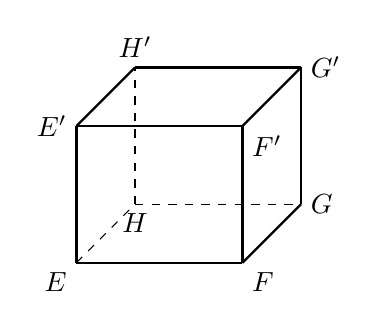
\begin{tikzpicture}[scale=0.62,>=stealth]
\draw[thick] (0,0)--(3.4,0);
\draw[thick] (3.4,0)--(4.6,1.2);
\draw[thick] (4.6,1.2)--(4.6,4.0);
\draw[thick] (0,2.8)--(3.4,2.8);
\draw[thick] (3.4,2.8)--(4.6,4.0);
\draw[thick] (4.6,4.0)--(1.2,4.0);
\draw[thick] (1.2,4.0)--(0,2.8);
\draw[thick] (0,0)--(0,2.8);
\draw[thick] (3.4,0)--(3.4,2.8);
\draw[dashed] (0,0)--(1.2,1.2);
\draw[dashed] (1.2,1.2)--(4.6,1.2);
\draw[dashed] (1.2,1.2)--(1.2,4.0);
\node[below left] at (0,0){$E$};
\node[below right] at (3.4,0){$F$};
\node[right] at (4.6,1.2){$G$};
\node[below] at (1.2,1.2){$H$};
\node[left] at (0,2.8){$E'$};
\node[below right] at (3.4,2.8){$F'$};
\node[right] at (4.6,4.0){$G'$};
\node[above] at (1.2,4.0){$H'$};
\end{tikzpicture}
\end{center}
 Vectơ nào dưới đây bằng vectơ $\overrightarrow{FG'}$?}
  {$\overrightarrow{EH'}$.}
  {$\overrightarrow{G'F}$.}{$\overrightarrow{GE}$.}{$\overrightarrow{GE'}$.}

\cauTN[id=C2-B6-D01-NB-004,muc=NB,loigiai={Hai vectơ bằng nhau khi chúng cùng hướng và cùng độ dài. Trong hình, $DHFB$ là hình bình hành (hai cạnh $DH$ và $BF$ song song, cùng hướng và bằng nhau) nên $\overrightarrow{DH}=\overrightarrow{BF}$. Các phương án còn lại là vectơ đối hoặc có hướng, độ dài khác $\overrightarrow{DH}$.}]{Cho hình hộp $ABCD.EFGH$. Vectơ nào dưới đây bằng vectơ $\overrightarrow{DH}$?}
  {$\overrightarrow{BF}$.}
  {$\overrightarrow{FB}$.}{$\overrightarrow{FA}$.}{$\overrightarrow{HE}$.}

\cauTN[id=C2-B6-D01-NB-005,muc=NB,loigiai={Hai vectơ bằng nhau khi chúng cùng hướng và cùng độ dài. Trong hình, $GDAF$ là hình bình hành (hai cạnh $GD$ và $FA$ song song, cùng hướng và bằng nhau) nên $\overrightarrow{GD}=\overrightarrow{FA}$. Các phương án còn lại là vectơ đối hoặc có hướng, độ dài khác $\overrightarrow{GD}$.}]{Cho hình hộp $ABCD.EFGH$. Vectơ nào dưới đây bằng vectơ $\overrightarrow{GD}$?}
  {$\overrightarrow{FA}$.}
  {$\overrightarrow{AF}$.}{$\overrightarrow{BE}$.}{$\overrightarrow{AH}$.}

\cauTN[id=C2-B6-D01-NB-006,muc=NB,loigiai={Hai vectơ bằng nhau khi chúng cùng hướng và cùng độ dài. Trong hình, $B'C'DA$ là hình bình hành (hai cạnh $B'C'$ và $AD$ song song, cùng hướng và bằng nhau) nên $\overrightarrow{B'C'}=\overrightarrow{AD}$. Các phương án còn lại là vectơ đối hoặc có hướng, độ dài khác $\overrightarrow{B'C'}$.}]{Cho hình hộp $ABCD.A'B'C'D'$ như hình vẽ.
\begin{center}
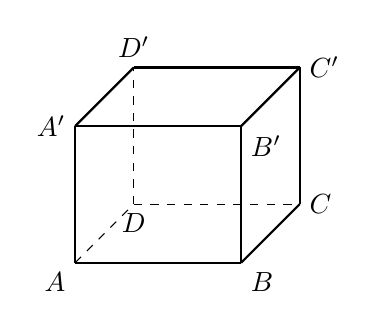
\begin{tikzpicture}[scale=0.62,>=stealth]
\draw[thick] (0,0)--(3.4,0);
\draw[thick] (3.4,0)--(4.6,1.2);
\draw[thick] (4.6,1.2)--(4.6,4.0);
\draw[thick] (0,2.8)--(3.4,2.8);
\draw[thick] (3.4,2.8)--(4.6,4.0);
\draw[thick] (4.6,4.0)--(1.2,4.0);
\draw[thick] (1.2,4.0)--(0,2.8);
\draw[thick] (0,0)--(0,2.8);
\draw[thick] (3.4,0)--(3.4,2.8);
\draw[dashed] (0,0)--(1.2,1.2);
\draw[dashed] (1.2,1.2)--(4.6,1.2);
\draw[dashed] (1.2,1.2)--(1.2,4.0);
\node[below left] at (0,0){$A$};
\node[below right] at (3.4,0){$B$};
\node[right] at (4.6,1.2){$C$};
\node[below] at (1.2,1.2){$D$};
\node[left] at (0,2.8){$A'$};
\node[below right] at (3.4,2.8){$B'$};
\node[right] at (4.6,4.0){$C'$};
\node[above] at (1.2,4.0){$D'$};
\end{tikzpicture}
\end{center}
 Vectơ nào dưới đây bằng vectơ $\overrightarrow{B'C'}$?}
  {$\overrightarrow{AD}$.}
  {$\overrightarrow{C'B'}$.}{$\overrightarrow{BA'}$.}{$\overrightarrow{D'C}$.}

\cauTN[id=C2-B6-D01-NB-007,muc=NB,loigiai={Hai vectơ bằng nhau khi chúng cùng hướng và cùng độ dài. Trong hình, $F'E'HG$ là hình bình hành (hai cạnh $F'E'$ và $GH$ song song, cùng hướng và bằng nhau) nên $\overrightarrow{F'E'}=\overrightarrow{GH}$. Các phương án còn lại là vectơ đối hoặc có hướng, độ dài khác $\overrightarrow{F'E'}$.}]{Cho hình hộp $EFGH.E'F'G'H'$. Vectơ nào dưới đây bằng vectơ $\overrightarrow{F'E'}$?}
  {$\overrightarrow{GH}$.}
  {$\overrightarrow{EF}$.}{$\overrightarrow{HH'}$.}{$\overrightarrow{G'E'}$.}

\cauTN[id=C2-B6-D01-NB-008,muc=NB,loigiai={Hai vectơ bằng nhau khi chúng cùng hướng và cùng độ dài. Trong hình, $FEH'G'$ là hình bình hành (hai cạnh $FE$ và $G'H'$ song song, cùng hướng và bằng nhau) nên $\overrightarrow{FE}=\overrightarrow{G'H'}$. Các phương án còn lại là vectơ đối hoặc có hướng, độ dài khác $\overrightarrow{FE}$.}]{Cho hình hộp $EFGH.E'F'G'H'$ như hình vẽ.
\begin{center}
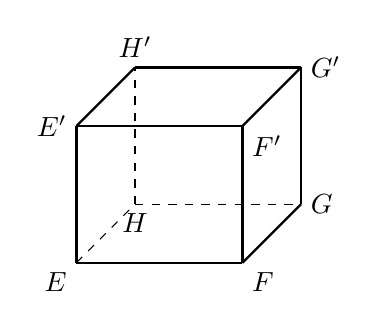
\begin{tikzpicture}[scale=0.62,>=stealth]
\draw[thick] (0,0)--(3.4,0);
\draw[thick] (3.4,0)--(4.6,1.2);
\draw[thick] (4.6,1.2)--(4.6,4.0);
\draw[thick] (0,2.8)--(3.4,2.8);
\draw[thick] (3.4,2.8)--(4.6,4.0);
\draw[thick] (4.6,4.0)--(1.2,4.0);
\draw[thick] (1.2,4.0)--(0,2.8);
\draw[thick] (0,0)--(0,2.8);
\draw[thick] (3.4,0)--(3.4,2.8);
\draw[dashed] (0,0)--(1.2,1.2);
\draw[dashed] (1.2,1.2)--(4.6,1.2);
\draw[dashed] (1.2,1.2)--(1.2,4.0);
\node[below left] at (0,0){$E$};
\node[below right] at (3.4,0){$F$};
\node[right] at (4.6,1.2){$G$};
\node[below] at (1.2,1.2){$H$};
\node[left] at (0,2.8){$E'$};
\node[below right] at (3.4,2.8){$F'$};
\node[right] at (4.6,4.0){$G'$};
\node[above] at (1.2,4.0){$H'$};
\end{tikzpicture}
\end{center}
 Vectơ nào dưới đây bằng vectơ $\overrightarrow{FE}$?}
  {$\overrightarrow{G'H'}$.}
  {$\overrightarrow{H'G'}$.}{$\overrightarrow{G'H}$.}{$\overrightarrow{EH}$.}

\cauTN[id=C2-B6-D01-NB-009,muc=NB,loigiai={Hai vectơ bằng nhau khi chúng cùng hướng và cùng độ dài. Trong hình, $ABC'D'$ là hình bình hành (hai cạnh $AB$ và $D'C'$ song song, cùng hướng và bằng nhau) nên $\overrightarrow{AB}=\overrightarrow{D'C'}$. Các phương án còn lại là vectơ đối hoặc có hướng, độ dài khác $\overrightarrow{AB}$.}]{Cho hình hộp $ABCD.A'B'C'D'$. Vectơ nào dưới đây bằng vectơ $\overrightarrow{AB}$?}
  {$\overrightarrow{D'C'}$.}
  {$\overrightarrow{C'D'}$.}{$\overrightarrow{C'D}$.}{$\overrightarrow{CA'}$.}

\cauTN[id=C2-B6-D01-NB-010,muc=NB,loigiai={Hai vectơ bằng nhau khi chúng cùng hướng và cùng độ dài. Trong hình, $M'N'NM$ là hình bình hành (hai cạnh $M'N'$ và $MN$ song song, cùng hướng và bằng nhau) nên $\overrightarrow{M'N'}=\overrightarrow{MN}$. Các phương án còn lại là vectơ đối hoặc có hướng, độ dài khác $\overrightarrow{M'N'}$.}]{Cho hình hộp $MNPQ.M'N'P'Q'$ như hình vẽ.
\begin{center}
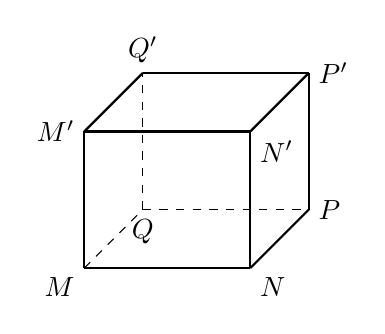
\begin{tikzpicture}[scale=0.62,>=stealth]
\draw[thick] (0,0)--(3.4,0);
\draw[thick] (3.4,0)--(4.6,1.2);
\draw[thick] (4.6,1.2)--(4.6,4.0);
\draw[thick] (0,2.8)--(3.4,2.8);
\draw[thick] (3.4,2.8)--(4.6,4.0);
\draw[thick] (4.6,4.0)--(1.2,4.0);
\draw[thick] (1.2,4.0)--(0,2.8);
\draw[thick] (0,0)--(0,2.8);
\draw[thick] (3.4,0)--(3.4,2.8);
\draw[dashed] (0,0)--(1.2,1.2);
\draw[dashed] (1.2,1.2)--(4.6,1.2);
\draw[dashed] (1.2,1.2)--(1.2,4.0);
\node[below left] at (0,0){$M$};
\node[below right] at (3.4,0){$N$};
\node[right] at (4.6,1.2){$P$};
\node[below] at (1.2,1.2){$Q$};
\node[left] at (0,2.8){$M'$};
\node[below right] at (3.4,2.8){$N'$};
\node[right] at (4.6,4.0){$P'$};
\node[above] at (1.2,4.0){$Q'$};
\end{tikzpicture}
\end{center}
 Vectơ nào dưới đây bằng vectơ $\overrightarrow{M'N'}$?}
  {$\overrightarrow{MN}$.}
  {$\overrightarrow{N'M'}$.}{$\overrightarrow{P'Q}$.}{$\overrightarrow{N'P'}$.}

\cauTN[id=C2-B6-D01-NB-011,muc=NB,loigiai={Vectơ đối của $\overrightarrow{CB}$ là vectơ có cùng độ dài và ngược hướng với $\overrightarrow{CB}$. Ta có $\overrightarrow{AD}=-\overrightarrow{CB}$ nên đáp án là $\overrightarrow{AD}$.}]{Cho hình chóp $S.ABCD$ có đáy $ABCD$ là hình bình hành như hình vẽ.
\begin{center}
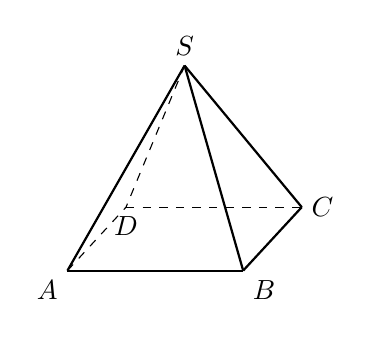
\begin{tikzpicture}[scale=0.62,>=stealth]
\draw[thick] (0,0)--(3.6,0);
\draw[thick] (3.6,0)--(4.8,1.3);
\draw[thick] (2.4,4.2)--(0,0);
\draw[thick] (2.4,4.2)--(3.6,0);
\draw[thick] (2.4,4.2)--(4.8,1.3);
\draw[dashed] (0,0)--(1.2,1.3);
\draw[dashed] (1.2,1.3)--(4.8,1.3);
\draw[dashed] (2.4,4.2)--(1.2,1.3);
\node[below left] at (0,0){$A$};
\node[below right] at (3.6,0){$B$};
\node[right] at (4.8,1.3){$C$};
\node[below] at (1.2,1.3){$D$};
\node[above] at (2.4,4.2){$S$};
\end{tikzpicture}
\end{center}
 Vectơ đối của vectơ $\overrightarrow{CB}$ là vectơ nào sau đây?}
  {$\overrightarrow{AD}$.}
  {$\overrightarrow{DA}$.}{$\overrightarrow{SC}$.}{$\overrightarrow{CS}$.}

\cauTN[id=C2-B6-D01-NB-012,muc=NB,loigiai={Vectơ đối của $\overrightarrow{DC'}$ là vectơ có cùng độ dài và ngược hướng với $\overrightarrow{DC'}$. Ta có $\overrightarrow{C'D}=-\overrightarrow{DC'}$ nên đáp án là $\overrightarrow{C'D}$.}]{Cho hình hộp $ABCD.A'B'C'D'$ như hình vẽ.
\begin{center}
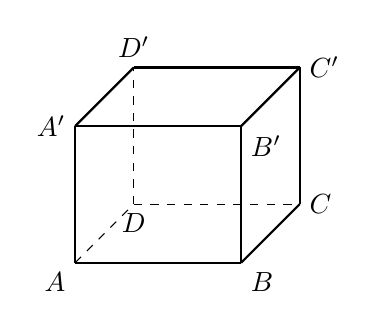
\begin{tikzpicture}[scale=0.62,>=stealth]
\draw[thick] (0,0)--(3.4,0);
\draw[thick] (3.4,0)--(4.6,1.2);
\draw[thick] (4.6,1.2)--(4.6,4.0);
\draw[thick] (0,2.8)--(3.4,2.8);
\draw[thick] (3.4,2.8)--(4.6,4.0);
\draw[thick] (4.6,4.0)--(1.2,4.0);
\draw[thick] (1.2,4.0)--(0,2.8);
\draw[thick] (0,0)--(0,2.8);
\draw[thick] (3.4,0)--(3.4,2.8);
\draw[dashed] (0,0)--(1.2,1.2);
\draw[dashed] (1.2,1.2)--(4.6,1.2);
\draw[dashed] (1.2,1.2)--(1.2,4.0);
\node[below left] at (0,0){$A$};
\node[below right] at (3.4,0){$B$};
\node[right] at (4.6,1.2){$C$};
\node[below] at (1.2,1.2){$D$};
\node[left] at (0,2.8){$A'$};
\node[below right] at (3.4,2.8){$B'$};
\node[right] at (4.6,4.0){$C'$};
\node[above] at (1.2,4.0){$D'$};
\end{tikzpicture}
\end{center}
 Vectơ đối của vectơ $\overrightarrow{DC'}$ là vectơ nào sau đây?}
  {$\overrightarrow{C'D}$.}
  {$\overrightarrow{DC'}$.}{$\overrightarrow{D'C}$.}{$\overrightarrow{AD}$.}

\cauTN[id=C2-B6-D01-NB-013,muc=NB,loigiai={Vectơ đối của $\overrightarrow{PM'}$ là vectơ có cùng độ dài và ngược hướng với $\overrightarrow{PM'}$. Ta có $\overrightarrow{M'P}=-\overrightarrow{PM'}$ nên đáp án là $\overrightarrow{M'P}$.}]{Cho hình hộp $MNPQ.M'N'P'Q'$. Vectơ đối của vectơ $\overrightarrow{PM'}$ là vectơ nào sau đây?}
  {$\overrightarrow{M'P}$.}
  {$\overrightarrow{PM'}$.}{$\overrightarrow{MQ'}$.}{$\overrightarrow{N'N}$.}

\cauTN[id=C2-B6-D01-NB-014,muc=NB,loigiai={Vectơ đối của $\overrightarrow{B'A}$ là vectơ có cùng độ dài và ngược hướng với $\overrightarrow{B'A}$. Ta có $\overrightarrow{DC'}=-\overrightarrow{B'A}$ nên đáp án là $\overrightarrow{DC'}$.}]{Cho hình hộp $ABCD.A'B'C'D'$. Vectơ đối của vectơ $\overrightarrow{B'A}$ là vectơ nào sau đây?}
  {$\overrightarrow{DC'}$.}
  {$\overrightarrow{C'D}$.}{$\overrightarrow{A'C}$.}{$\overrightarrow{BA}$.}

\cauTN[id=C2-B6-D01-NB-015,muc=NB,loigiai={Vectơ đối của $\overrightarrow{B'C'}$ là vectơ có cùng độ dài và ngược hướng với $\overrightarrow{B'C'}$. Ta có $\overrightarrow{C'B'}=-\overrightarrow{B'C'}$ nên đáp án là $\overrightarrow{C'B'}$.}]{Cho hình hộp $ABCD.A'B'C'D'$. Vectơ đối của vectơ $\overrightarrow{B'C'}$ là vectơ nào sau đây?}
  {$\overrightarrow{C'B'}$.}
  {$\overrightarrow{AD}$.}{$\overrightarrow{DB}$.}{$\overrightarrow{BA}$.}

\cauTN[id=C2-B6-D01-NB-016,muc=NB,loigiai={Vectơ đối của $\overrightarrow{HG}$ là vectơ có cùng độ dài và ngược hướng với $\overrightarrow{HG}$. Ta có $\overrightarrow{FE}=-\overrightarrow{HG}$ nên đáp án là $\overrightarrow{FE}$.}]{Cho hình hộp $ABCD.EFGH$. Vectơ đối của vectơ $\overrightarrow{HG}$ là vectơ nào sau đây?}
  {$\overrightarrow{FE}$.}
  {$\overrightarrow{AB}$.}{$\overrightarrow{CB}$.}{$\overrightarrow{EA}$.}

\cauTN[id=C2-B6-D01-NB-017,muc=NB,loigiai={Áp dụng quy tắc hình bình hành ta có $\overrightarrow{BC}+\overrightarrow{BF}=\overrightarrow{BG}$.}]{Cho hình hộp $ABCD.EFGH$ như hình vẽ.
\begin{center}
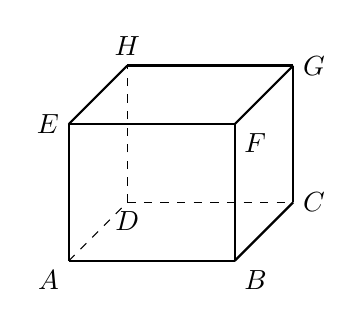
\begin{tikzpicture}[scale=0.62,>=stealth]
\draw[thick] (0,0)--(3.4,0);
\draw[thick] (3.4,0)--(4.6,1.2);
\draw[thick] (4.6,1.2)--(4.6,4.0);
\draw[thick] (0,2.8)--(3.4,2.8);
\draw[thick] (3.4,2.8)--(4.6,4.0);
\draw[thick] (4.6,4.0)--(1.2,4.0);
\draw[thick] (1.2,4.0)--(0,2.8);
\draw[thick] (0,0)--(0,2.8);
\draw[thick] (3.4,0)--(3.4,2.8);
\draw[dashed] (0,0)--(1.2,1.2);
\draw[dashed] (1.2,1.2)--(4.6,1.2);
\draw[dashed] (1.2,1.2)--(1.2,4.0);
\node[below left] at (0,0){$A$};
\node[below right] at (3.4,0){$B$};
\node[right] at (4.6,1.2){$C$};
\node[below] at (1.2,1.2){$D$};
\node[left] at (0,2.8){$E$};
\node[below right] at (3.4,2.8){$F$};
\node[right] at (4.6,4.0){$G$};
\node[above] at (1.2,4.0){$H$};
\end{tikzpicture}
\end{center}
 Tổng $\overrightarrow{BC}+\overrightarrow{BF}$ bằng vectơ nào sau đây?}
  {$\overrightarrow{BG}$.}
  {$\overrightarrow{GB}$.}{$\overrightarrow{FC}$.}{$\overrightarrow{GH}$.}

\cauTN[id=C2-B6-D01-NB-018,muc=NB,loigiai={Áp dụng quy tắc ba điểm ta có $\overrightarrow{BC}+\overrightarrow{CA}=\overrightarrow{CD}$.}]{Cho hình chóp $O.ABCD$ có đáy $ABCD$ là hình bình hành. Tổng $\overrightarrow{BC}+\overrightarrow{CA}$ bằng vectơ nào sau đây?}
  {$\overrightarrow{CD}$.}
  {$\overrightarrow{DC}$.}{$\overrightarrow{BD}$.}{$\overrightarrow{AC}$.}

\cauTN[id=C2-B6-D01-NB-019,muc=NB,loigiai={Áp dụng quy tắc hình bình hành ta có $\overrightarrow{DC}+\overrightarrow{DA}=\overrightarrow{DB}$.}]{Cho hình chóp $O.ABCD$ có đáy $ABCD$ là hình bình hành như hình vẽ.
\begin{center}
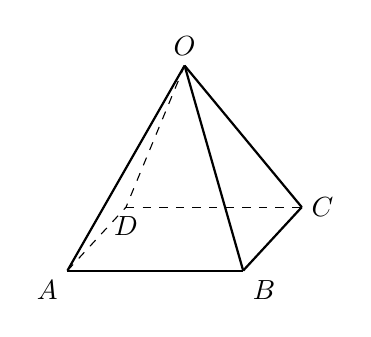
\begin{tikzpicture}[scale=0.62,>=stealth]
\draw[thick] (0,0)--(3.6,0);
\draw[thick] (3.6,0)--(4.8,1.3);
\draw[thick] (2.4,4.2)--(0,0);
\draw[thick] (2.4,4.2)--(3.6,0);
\draw[thick] (2.4,4.2)--(4.8,1.3);
\draw[dashed] (0,0)--(1.2,1.3);
\draw[dashed] (1.2,1.3)--(4.8,1.3);
\draw[dashed] (2.4,4.2)--(1.2,1.3);
\node[below left] at (0,0){$A$};
\node[below right] at (3.6,0){$B$};
\node[right] at (4.8,1.3){$C$};
\node[below] at (1.2,1.3){$D$};
\node[above] at (2.4,4.2){$O$};
\end{tikzpicture}
\end{center}
 Tổng $\overrightarrow{DC}+\overrightarrow{DA}$ bằng vectơ nào sau đây?}
  {$\overrightarrow{DB}$.}
  {$\overrightarrow{BD}$.}{$\overrightarrow{BO}$.}{$\overrightarrow{AD}$.}

\cauTN[id=C2-B6-D01-NB-020,muc=NB,loigiai={Áp dụng quy tắc ba điểm ta có $\overrightarrow{MP}-\overrightarrow{QP}=\overrightarrow{MQ}$.}]{Cho hình chóp $S.MNPQ$ có đáy $MNPQ$ là hình bình hành. Tổng $\overrightarrow{MP}-\overrightarrow{QP}$ bằng vectơ nào sau đây?}
  {$\overrightarrow{MQ}$.}
  {$\overrightarrow{QM}$.}{$\overrightarrow{SQ}$.}{$\overrightarrow{NS}$.}

\cauTN[id=C2-B6-D01-NB-021,muc=NB,loigiai={Áp dụng quy tắc ba điểm ta có $\overrightarrow{BA}+\overrightarrow{AF}=\overrightarrow{CG}$.}]{Cho hình hộp $ABCD.EFGH$. Tổng $\overrightarrow{BA}+\overrightarrow{AF}$ bằng vectơ nào sau đây?}
  {$\overrightarrow{CG}$.}
  {$\overrightarrow{GC}$.}{$\overrightarrow{FC}$.}{$\overrightarrow{EF}$.}

\cauTN[id=C2-B6-D01-NB-022,muc=NB,loigiai={Áp dụng quy tắc hình bình hành ta có $\overrightarrow{GH}+\overrightarrow{GF}=\overrightarrow{CA}$.}]{Cho hình hộp $ABCD.EFGH$. Tổng $\overrightarrow{GH}+\overrightarrow{GF}$ bằng vectơ nào sau đây?}
  {$\overrightarrow{CA}$.}
  {$\overrightarrow{AC}$.}{$\overrightarrow{GD}$.}{$\overrightarrow{GF}$.}

\cauTN[id=C2-B6-D01-NB-023,muc=NB,loigiai={Áp dụng quy tắc ba điểm ta có $\overrightarrow{SA}-\overrightarrow{BA}=\overrightarrow{SB}$.}]{Cho tứ diện $SABC$ như hình vẽ.
\begin{center}
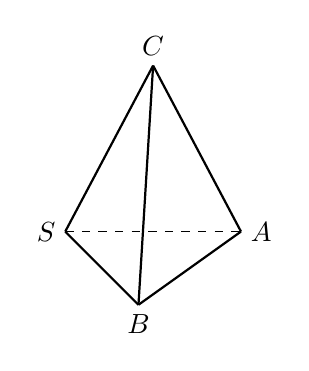
\begin{tikzpicture}[scale=0.62,>=stealth]
\draw[thick] (0,0)--(1.5,-1.5);
\draw[thick] (3.6,0)--(1.5,-1.5);
\draw[thick] (1.8,3.4)--(0,0);
\draw[thick] (1.8,3.4)--(3.6,0);
\draw[thick] (1.8,3.4)--(1.5,-1.5);
\draw[dashed] (0,0)--(3.6,0);
\node[left] at (0,0){$S$};
\node[right] at (3.6,0){$A$};
\node[below] at (1.5,-1.5){$B$};
\node[above] at (1.8,3.4){$C$};
\end{tikzpicture}
\end{center}
 Tổng $\overrightarrow{SA}-\overrightarrow{BA}$ bằng vectơ nào sau đây?}
  {$\overrightarrow{SB}$.}
  {$\overrightarrow{BS}$.}{$\overrightarrow{AS}$.}{$\overrightarrow{CB}$.}

\cauTN[id=C2-B6-D01-NB-024,muc=NB,loigiai={Áp dụng quy tắc ba điểm ta có $\overrightarrow{AD}+\overrightarrow{DG}=\overrightarrow{AG}$.}]{Cho hình hộp $ABCD.EFGH$. Tổng $\overrightarrow{AD}+\overrightarrow{DG}$ bằng vectơ nào sau đây?}
  {$\overrightarrow{AG}$.}
  {$\overrightarrow{GA}$.}{$\overrightarrow{BH}$.}{$\overrightarrow{BA}$.}

\cauTN[id=C2-B6-D01-NB-025,muc=NB,loigiai={Áp dụng quy tắc ba điểm ta có $\overrightarrow{BC}+\overrightarrow{CA}=\overrightarrow{BA}$.}]{Cho tứ diện $SABC$. Tổng $\overrightarrow{BC}+\overrightarrow{CA}$ bằng vectơ nào sau đây?}
  {$\overrightarrow{BA}$.}
  {$\overrightarrow{AB}$.}{$\overrightarrow{AC}$.}{$\overrightarrow{SB}$.}

\cauTN[id=C2-B6-D01-NB-026,muc=NB,loigiai={Áp dụng quy tắc hình bình hành ta có $\overrightarrow{FG'}+\overrightarrow{FE}=\overrightarrow{FH'}$.}]{Cho hình hộp $EFGH.E'F'G'H'$. Tổng $\overrightarrow{FG'}+\overrightarrow{FE}$ bằng vectơ nào sau đây?}
  {$\overrightarrow{FH'}$.}
  {$\overrightarrow{H'F}$.}{$\overrightarrow{FE'}$.}{$\overrightarrow{F'E'}$.}

\cauTN[id=C2-B6-D01-NB-027,muc=NB,loigiai={Sử dụng các quy tắc cộng, trừ vectơ trong không gian ta có $\overrightarrow{MS}-\overrightarrow{PS}=\overrightarrow{MP}$ là khẳng định đúng. Các khẳng định còn lại sai do hệ số hoặc chiều của vectơ không phù hợp.}]{Cho hình chóp $S.MNPQ$ có đáy $MNPQ$ là hình bình hành.  Khẳng định nào dưới đây đúng?}
  {$\overrightarrow{MS}-\overrightarrow{PS}=\overrightarrow{MP}$.}
  {$\overrightarrow{PS}-\overrightarrow{MS}=\overrightarrow{PN}$.}{$\overrightarrow{MQ}-\overrightarrow{SQ}=\overrightarrow{MN}$.}{$\overrightarrow{QS}-\overrightarrow{PS}=\overrightarrow{QS}$.}

\cauTN[id=C2-B6-D01-NB-028,muc=NB,loigiai={Sử dụng các quy tắc cộng, trừ vectơ trong không gian ta có $\overrightarrow{M'M}+\overrightarrow{MP}=\overrightarrow{M'P}$ là khẳng định đúng. Các khẳng định còn lại sai do hệ số hoặc chiều của vectơ không phù hợp.}]{Cho hình hộp $MNPQ.M'N'P'Q'$.  Khẳng định nào dưới đây đúng?}
  {$\overrightarrow{M'M}+\overrightarrow{MP}=\overrightarrow{M'P}$.}
  {$\overrightarrow{N'P'}-\overrightarrow{QP'}=\overrightarrow{N'N}$.}{$\overrightarrow{N'Q'}-\overrightarrow{NQ'}=\overrightarrow{N'M'}$.}{$\overrightarrow{PQ'}+\overrightarrow{Q'M'}=\overrightarrow{PN'}$.}

\cauTN[id=C2-B6-D01-NB-029,muc=NB,loigiai={Sử dụng tính chất trung điểm ($\overrightarrow{IX}+\overrightarrow{IY}=\overrightarrow{0}$; $\overrightarrow{OX}+\overrightarrow{OY}=2\overrightarrow{OI}$) ta có $\overrightarrow{IP}=-\overrightarrow{IP'}$ là khẳng định đúng. Các khẳng định còn lại sai do hệ số hoặc chiều của vectơ không phù hợp.}]{Cho hình hộp $MNPQ.M'N'P'Q'$. Gọi $I$ là trung điểm của đoạn thẳng $PP'$. Khẳng định nào dưới đây đúng?}
  {$\overrightarrow{IP}=-\overrightarrow{IP'}$.}
  {$\overrightarrow{MP}+\overrightarrow{MP'}=\overrightarrow{MI}$.}{$\overrightarrow{PP'}=2\overrightarrow{IP}$.}{$\overrightarrow{IP}=\overrightarrow{IP'}$.}

\cauTN[id=C2-B6-D01-NB-030,muc=NB,loigiai={Sử dụng tính chất trọng tâm tam giác ta có $\overrightarrow{PG}=\dfrac{1}{3}\overrightarrow{PQ}+\dfrac{1}{3}\overrightarrow{PM}$ là khẳng định đúng. Các khẳng định còn lại sai do hệ số hoặc chiều của vectơ không phù hợp.}]{Cho tứ diện $MNPQ$. Gọi $G$ là trọng tâm của tam giác $PQM$. Khẳng định nào dưới đây đúng?}
  {$\overrightarrow{PG}=\dfrac{1}{3}\overrightarrow{PQ}+\dfrac{1}{3}\overrightarrow{PM}$.}
  {$\overrightarrow{GP}+\overrightarrow{GQ}=\overrightarrow{GM}$.}{$\overrightarrow{NP}+\overrightarrow{NQ}+\overrightarrow{NM}=\overrightarrow{NG}$.}{$\overrightarrow{PG}=\dfrac{1}{2}\overrightarrow{PQ}+\dfrac{1}{2}\overrightarrow{PM}$.}

\cauTN[id=C2-B6-D01-NB-031,muc=NB,loigiai={Sử dụng tính chất trung điểm ($\overrightarrow{IX}+\overrightarrow{IY}=\overrightarrow{0}$; $\overrightarrow{OX}+\overrightarrow{OY}=2\overrightarrow{OI}$) ta có $\overrightarrow{NI}=\dfrac{1}{2}\overrightarrow{NQ}$ là khẳng định đúng. Các khẳng định còn lại sai do hệ số hoặc chiều của vectơ không phù hợp.}]{Cho tứ diện $MNPQ$ như hình vẽ.
\begin{center}
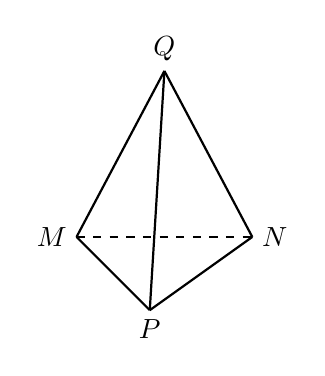
\begin{tikzpicture}[scale=0.62,>=stealth]
\draw[thick] (0,0)--(1.5,-1.5);
\draw[thick] (3.6,0)--(1.5,-1.5);
\draw[thick] (1.8,3.4)--(0,0);
\draw[thick] (1.8,3.4)--(3.6,0);
\draw[thick] (1.8,3.4)--(1.5,-1.5);
\draw[dashed] (0,0)--(3.6,0);
\node[left] at (0,0){$M$};
\node[right] at (3.6,0){$N$};
\node[below] at (1.5,-1.5){$P$};
\node[above] at (1.8,3.4){$Q$};
\end{tikzpicture}
\end{center}
Gọi $I$ là trung điểm của đoạn thẳng $NQ$.  Khẳng định nào dưới đây đúng?}
  {$\overrightarrow{NI}=\dfrac{1}{2}\overrightarrow{NQ}$.}
  {$\overrightarrow{IN}=\overrightarrow{IQ}$.}{$\overrightarrow{MN}+\overrightarrow{MQ}=\overrightarrow{MI}$.}{$\overrightarrow{PN}+\overrightarrow{PQ}=\overrightarrow{PI}$.}

\cauTN[id=C2-B6-D01-NB-032,muc=NB,loigiai={Sử dụng tính chất trung điểm ($\overrightarrow{IX}+\overrightarrow{IY}=\overrightarrow{0}$; $\overrightarrow{OX}+\overrightarrow{OY}=2\overrightarrow{OI}$) ta có $\overrightarrow{C'D}+\overrightarrow{C'B}=2\overrightarrow{C'I}$ là khẳng định đúng. Các khẳng định còn lại sai do hệ số hoặc chiều của vectơ không phù hợp.}]{Cho hình hộp $ABCD.A'B'C'D'$. Gọi $I$ là trung điểm của đoạn thẳng $DB$. Khẳng định nào dưới đây đúng?}
  {$\overrightarrow{C'D}+\overrightarrow{C'B}=2\overrightarrow{C'I}$.}
  {$\overrightarrow{ID}=\overrightarrow{IB}$.}{$\overrightarrow{AD}+\overrightarrow{AB}=3\overrightarrow{AI}$.}{$\overrightarrow{A'D}+\overrightarrow{A'B}=\overrightarrow{A'I}$.}

\cauTN[id=C2-B6-D01-NB-033,muc=NB,loigiai={Sử dụng tính chất trọng tâm tam giác ta có $\overrightarrow{DG}=\dfrac{1}{3}\overrightarrow{DA}+\dfrac{1}{3}\overrightarrow{DC}$ là khẳng định đúng. Các khẳng định còn lại sai do hệ số hoặc chiều của vectơ không phù hợp.}]{Cho hình chóp $O.ABCD$ có đáy $ABCD$ là hình bình hành. Gọi $G$ là trọng tâm của tam giác $DAC$. Khẳng định nào dưới đây đúng?}
  {$\overrightarrow{DG}=\dfrac{1}{3}\overrightarrow{DA}+\dfrac{1}{3}\overrightarrow{DC}$.}
  {$\overrightarrow{BD}+\overrightarrow{BA}+\overrightarrow{BC}=2\overrightarrow{BG}$.}{$\overrightarrow{DG}=\dfrac{1}{2}\overrightarrow{DA}+\dfrac{1}{2}\overrightarrow{DC}$.}{$\overrightarrow{OD}+\overrightarrow{OA}+\overrightarrow{OC}=\overrightarrow{OG}$.}

\cauTN[id=C2-B6-D01-NB-034,muc=NB,loigiai={Sử dụng tính chất trọng tâm tam giác ta có $\overrightarrow{GB'}+\overrightarrow{GA}+\overrightarrow{GD}=\overrightarrow{0}$ là khẳng định đúng. Các khẳng định còn lại sai do hệ số hoặc chiều của vectơ không phù hợp.}]{Cho hình hộp $ABCD.A'B'C'D'$. Gọi $G$ là trọng tâm của tam giác $B'AD$. Khẳng định nào dưới đây đúng?}
  {$\overrightarrow{GB'}+\overrightarrow{GA}+\overrightarrow{GD}=\overrightarrow{0}$.}
  {$\overrightarrow{BB'}+\overrightarrow{BA}+\overrightarrow{BD}=2\overrightarrow{BG}$.}{$\overrightarrow{GB'}=\overrightarrow{GA}+\overrightarrow{GD}$.}{$\overrightarrow{C'B'}+\overrightarrow{C'A}+\overrightarrow{C'D}=\overrightarrow{C'G}$.}

\cauTN[id=C2-B6-D01-NB-035,muc=NB,loigiai={Sử dụng các quy tắc cộng, trừ vectơ trong không gian ta có $\overrightarrow{GC}-\overrightarrow{EC}=\overrightarrow{GE}$ là khẳng định đúng. Các khẳng định còn lại sai do hệ số hoặc chiều của vectơ không phù hợp.}]{Cho hình hộp $ABCD.EFGH$.  Khẳng định nào dưới đây đúng?}
  {$\overrightarrow{GC}-\overrightarrow{EC}=\overrightarrow{GE}$.}
  {$\overrightarrow{HC}+\overrightarrow{CF}=\overrightarrow{HB}$.}{$\overrightarrow{CD}+\overrightarrow{DB}=\overrightarrow{CG}$.}{$\overrightarrow{BD}+\overrightarrow{DG}=\overrightarrow{BE}$.}

\cauTN[id=C2-B6-D01-NB-036,muc=NB,loigiai={Sử dụng tính chất trung điểm ($\overrightarrow{IX}+\overrightarrow{IY}=\overrightarrow{0}$; $\overrightarrow{OX}+\overrightarrow{OY}=2\overrightarrow{OI}$) ta có $\overrightarrow{CD}+\overrightarrow{CA}=2\overrightarrow{CI}$ là khẳng định đúng. Các khẳng định còn lại sai do hệ số hoặc chiều của vectơ không phù hợp.}]{Cho hình chóp $O.ABCD$ có đáy $ABCD$ là hình bình hành như hình vẽ.
\begin{center}
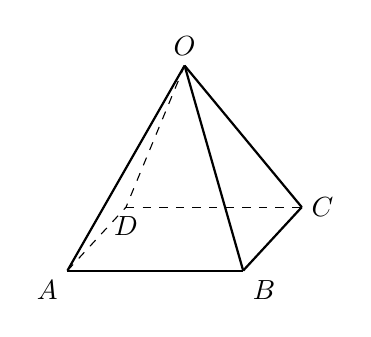
\begin{tikzpicture}[scale=0.62,>=stealth]
\draw[thick] (0,0)--(3.6,0);
\draw[thick] (3.6,0)--(4.8,1.3);
\draw[thick] (2.4,4.2)--(0,0);
\draw[thick] (2.4,4.2)--(3.6,0);
\draw[thick] (2.4,4.2)--(4.8,1.3);
\draw[dashed] (0,0)--(1.2,1.3);
\draw[dashed] (1.2,1.3)--(4.8,1.3);
\draw[dashed] (2.4,4.2)--(1.2,1.3);
\node[below left] at (0,0){$A$};
\node[below right] at (3.6,0){$B$};
\node[right] at (4.8,1.3){$C$};
\node[below] at (1.2,1.3){$D$};
\node[above] at (2.4,4.2){$O$};
\end{tikzpicture}
\end{center}
Gọi $I$ là trung điểm của đoạn thẳng $DA$.  Khẳng định nào dưới đây đúng?}
  {$\overrightarrow{CD}+\overrightarrow{CA}=2\overrightarrow{CI}$.}
  {$\overrightarrow{CD}+\overrightarrow{CA}=\overrightarrow{CI}$.}{$\overrightarrow{DA}=2\overrightarrow{ID}$.}{$\overrightarrow{ID}=\overrightarrow{IA}$.}

\cauDS[id=C2-B6-D01-NB-037,muc=NB,loigiai={Áp dụng quy tắc ba điểm, quy tắc hình bình hành, quy tắc hình hộp và định nghĩa hai vectơ bằng nhau. a) Đúng. b) Đúng. c) Đúng. d) Sai.}]{Cho hình chóp $O.ABCD$ có đáy $ABCD$ là hình bình hành như hình vẽ.
\begin{center}
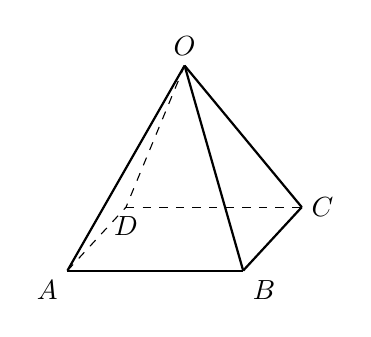
\begin{tikzpicture}[scale=0.62,>=stealth]
\draw[thick] (0,0)--(3.6,0);
\draw[thick] (3.6,0)--(4.8,1.3);
\draw[thick] (2.4,4.2)--(0,0);
\draw[thick] (2.4,4.2)--(3.6,0);
\draw[thick] (2.4,4.2)--(4.8,1.3);
\draw[dashed] (0,0)--(1.2,1.3);
\draw[dashed] (1.2,1.3)--(4.8,1.3);
\draw[dashed] (2.4,4.2)--(1.2,1.3);
\node[below left] at (0,0){$A$};
\node[below right] at (3.6,0){$B$};
\node[right] at (4.8,1.3){$C$};
\node[below] at (1.2,1.3){$D$};
\node[above] at (2.4,4.2){$O$};
\end{tikzpicture}
\end{center}
  Xét tính đúng sai của các mệnh đề sau:}{%
  \y{$\overrightarrow{OC}-\overrightarrow{AC}=\overrightarrow{OA}$.}{d}
  \y{$\overrightarrow{BD}+\overrightarrow{DC}=\overrightarrow{BC}$.}{d}
  \y{$\overrightarrow{CO}+\overrightarrow{OD}=\overrightarrow{CD}$.}{d}
  \y{$\overrightarrow{AO}=\overrightarrow{OB}$.}{s}}

\cauDS[id=C2-B6-D01-NB-038,muc=NB,loigiai={Áp dụng quy tắc ba điểm, quy tắc hình bình hành, quy tắc hình hộp và định nghĩa hai vectơ bằng nhau. a) Sai. b) Sai. c) Sai. d) Đúng.}]{Cho hình hộp $ABCD.A'B'C'D'$.  Xét tính đúng sai của các mệnh đề sau:}{%
  \y{$\overrightarrow{B'D}=\overrightarrow{DB}$.}{s}
  \y{$\overrightarrow{B'D'}+\overrightarrow{D'C'}=\overrightarrow{B'A'}$.}{s}
  \y{$\overrightarrow{AA'}+\overrightarrow{AB}+\overrightarrow{AD}=\overrightarrow{AB}$.}{s}
  \y{$\overrightarrow{BA'}=-\overrightarrow{D'C}$.}{d}}

\cauDS[id=C2-B6-D01-NB-039,muc=NB,loigiai={Áp dụng quy tắc ba điểm, quy tắc hình bình hành, quy tắc hình hộp và định nghĩa hai vectơ bằng nhau. a) Đúng. b) Sai. c) Sai. d) Sai.}]{Cho hình hộp $MNPQ.M'N'P'Q'$.  Xét tính đúng sai của các mệnh đề sau:}{%
  \y{$\overrightarrow{QM}+\overrightarrow{QP'}=\overrightarrow{QN'}$.}{d}
  \y{$\overrightarrow{N'P'}+\overrightarrow{N'M'}+\overrightarrow{N'N}=\overrightarrow{N'P}$.}{s}
  \y{$\overrightarrow{N'P'}+\overrightarrow{N'M'}=\overrightarrow{N'Q}$.}{s}
  \y{$\overrightarrow{Q'P}+\overrightarrow{Q'M'}=\overrightarrow{Q'M}$.}{s}}

\cauDS[id=C2-B6-D01-NB-040,muc=NB,loigiai={Áp dụng quy tắc ba điểm, quy tắc hình bình hành, quy tắc hình hộp và định nghĩa hai vectơ bằng nhau. a) Sai. b) Sai. c) Sai. d) Đúng.}]{Cho hình hộp $ABCD.EFGH$ như hình vẽ.
\begin{center}
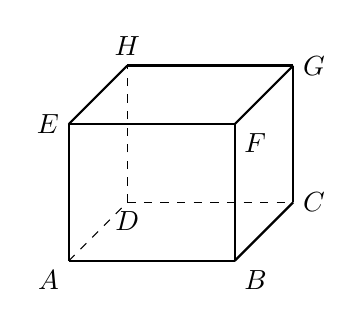
\begin{tikzpicture}[scale=0.62,>=stealth]
\draw[thick] (0,0)--(3.4,0);
\draw[thick] (3.4,0)--(4.6,1.2);
\draw[thick] (4.6,1.2)--(4.6,4.0);
\draw[thick] (0,2.8)--(3.4,2.8);
\draw[thick] (3.4,2.8)--(4.6,4.0);
\draw[thick] (4.6,4.0)--(1.2,4.0);
\draw[thick] (1.2,4.0)--(0,2.8);
\draw[thick] (0,0)--(0,2.8);
\draw[thick] (3.4,0)--(3.4,2.8);
\draw[dashed] (0,0)--(1.2,1.2);
\draw[dashed] (1.2,1.2)--(4.6,1.2);
\draw[dashed] (1.2,1.2)--(1.2,4.0);
\node[below left] at (0,0){$A$};
\node[below right] at (3.4,0){$B$};
\node[right] at (4.6,1.2){$C$};
\node[below] at (1.2,1.2){$D$};
\node[left] at (0,2.8){$E$};
\node[below right] at (3.4,2.8){$F$};
\node[right] at (4.6,4.0){$G$};
\node[above] at (1.2,4.0){$H$};
\end{tikzpicture}
\end{center}
  Xét tính đúng sai của các mệnh đề sau:}{%
  \y{$\overrightarrow{CG}+\overrightarrow{CB}=\overrightarrow{CE}$.}{s}
  \y{$\overrightarrow{FG}+\overrightarrow{FE}+\overrightarrow{FB}=\overrightarrow{FE}$.}{s}
  \y{$\overrightarrow{FD}=\overrightarrow{GD}$.}{s}
  \y{$\overrightarrow{HG}+\overrightarrow{HE}+\overrightarrow{HD}=\overrightarrow{HB}$.}{d}}

\cauDS[id=C2-B6-D01-NB-041,muc=NB,loigiai={Áp dụng quy tắc ba điểm, quy tắc hình bình hành, quy tắc hình hộp và định nghĩa hai vectơ bằng nhau. a) Sai. b) Sai. c) Đúng. d) Đúng.}]{Cho hình hộp $ABCD.EFGH$.  Xét tính đúng sai của các mệnh đề sau:}{%
  \y{$\overrightarrow{DH}+\overrightarrow{DA}+\overrightarrow{DC}=\overrightarrow{DA}$.}{s}
  \y{$\overrightarrow{ED}=\overrightarrow{AH}$.}{s}
  \y{$\overrightarrow{AE}+\overrightarrow{AC}=\overrightarrow{AG}$.}{d}
  \y{$\overrightarrow{FB}+\overrightarrow{FG}+\overrightarrow{FE}=\overrightarrow{FD}$.}{d}}

\cauDS[id=C2-B6-D01-NB-042,muc=NB,loigiai={Áp dụng quy tắc ba điểm, quy tắc hình bình hành, quy tắc hình hộp và định nghĩa hai vectơ bằng nhau. a) Sai. b) Đúng. c) Sai. d) Sai.}]{Cho tứ diện $ABCD$ như hình vẽ.
\begin{center}
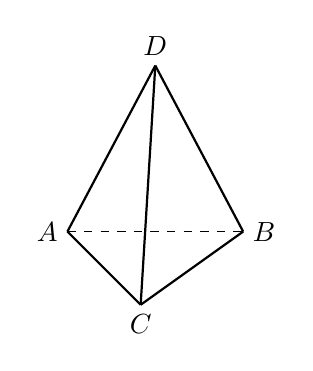
\begin{tikzpicture}[scale=0.62,>=stealth]
\draw[thick] (0,0)--(1.5,-1.5);
\draw[thick] (3.6,0)--(1.5,-1.5);
\draw[thick] (1.8,3.4)--(0,0);
\draw[thick] (1.8,3.4)--(3.6,0);
\draw[thick] (1.8,3.4)--(1.5,-1.5);
\draw[dashed] (0,0)--(3.6,0);
\node[left] at (0,0){$A$};
\node[right] at (3.6,0){$B$};
\node[below] at (1.5,-1.5){$C$};
\node[above] at (1.8,3.4){$D$};
\end{tikzpicture}
\end{center}
  Xét tính đúng sai của các mệnh đề sau:}{%
  \y{$\overrightarrow{DA}=-\overrightarrow{BC}$.}{s}
  \y{$\overrightarrow{DC}+\overrightarrow{CA}=\overrightarrow{DA}$.}{d}
  \y{$\overrightarrow{BC}=\overrightarrow{CD}$.}{s}
  \y{$\overrightarrow{CD}=\overrightarrow{AC}$.}{s}}

\cauDS[id=C2-B6-D01-NB-043,muc=NB,loigiai={Áp dụng quy tắc ba điểm, quy tắc hình bình hành, quy tắc hình hộp và định nghĩa hai vectơ bằng nhau. a) Đúng. b) Sai. c) Đúng. d) Sai.}]{Cho hình hộp $EFGH.E'F'G'H'$.  Xét tính đúng sai của các mệnh đề sau:}{%
  \y{$\overrightarrow{H'E'}+\overrightarrow{H'G'}+\overrightarrow{H'H}=\overrightarrow{H'F}$.}{d}
  \y{$\overrightarrow{H'F}+\overrightarrow{FE'}=\overrightarrow{H'E}$.}{s}
  \y{$\overrightarrow{G'E'}+\overrightarrow{G'G}=\overrightarrow{G'E}$.}{d}
  \y{$\overrightarrow{E'H}-\overrightarrow{F'H}=\overrightarrow{E'G'}$.}{s}}

\cauDS[id=C2-B6-D01-NB-044,muc=NB,loigiai={Áp dụng quy tắc ba điểm, quy tắc hình bình hành, quy tắc hình hộp và định nghĩa hai vectơ bằng nhau. a) Đúng. b) Đúng. c) Sai. d) Đúng.}]{Cho tứ diện $MNPQ$ như hình vẽ.
\begin{center}
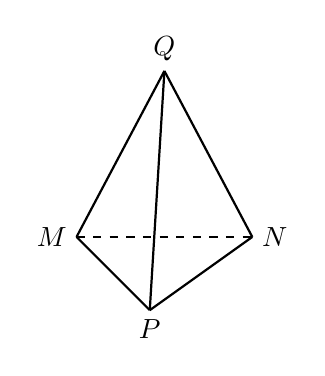
\begin{tikzpicture}[scale=0.62,>=stealth]
\draw[thick] (0,0)--(1.5,-1.5);
\draw[thick] (3.6,0)--(1.5,-1.5);
\draw[thick] (1.8,3.4)--(0,0);
\draw[thick] (1.8,3.4)--(3.6,0);
\draw[thick] (1.8,3.4)--(1.5,-1.5);
\draw[dashed] (0,0)--(3.6,0);
\node[left] at (0,0){$M$};
\node[right] at (3.6,0){$N$};
\node[below] at (1.5,-1.5){$P$};
\node[above] at (1.8,3.4){$Q$};
\end{tikzpicture}
\end{center}
  Xét tính đúng sai của các mệnh đề sau:}{%
  \y{$\overrightarrow{PQ}=-\overrightarrow{QP}$.}{d}
  \y{$\overrightarrow{QM}-\overrightarrow{NM}=\overrightarrow{QN}$.}{d}
  \y{$\overrightarrow{QM}-\overrightarrow{PM}=\overrightarrow{QN}$.}{s}
  \y{$\overrightarrow{NQ}=-\overrightarrow{QN}$.}{d}}

\cauDS[id=C2-B6-D01-NB-045,muc=NB,loigiai={Áp dụng quy tắc ba điểm, quy tắc hình bình hành, quy tắc hình hộp và định nghĩa hai vectơ bằng nhau. a) Đúng. b) Đúng. c) Sai. d) Đúng.}]{Cho hình chóp $S.MNPQ$ có đáy $MNPQ$ là hình bình hành.  Xét tính đúng sai của các mệnh đề sau:}{%
  \y{$\overrightarrow{SM}=-\overrightarrow{MS}$.}{d}
  \y{$\overrightarrow{NP}=-\overrightarrow{PN}$.}{d}
  \y{$\overrightarrow{NM}-\overrightarrow{SM}=\overrightarrow{NM}$.}{s}
  \y{$\overrightarrow{QS}-\overrightarrow{NS}=\overrightarrow{QN}$.}{d}}

\cauDS[id=C2-B6-D01-NB-046,muc=NB,loigiai={Áp dụng quy tắc ba điểm, quy tắc hình bình hành, quy tắc hình hộp và định nghĩa hai vectơ bằng nhau. a) Sai. b) Đúng. c) Đúng. d) Sai.}]{Cho hình hộp $MNPQ.M'N'P'Q'$.  Xét tính đúng sai của các mệnh đề sau:}{%
  \y{$\overrightarrow{P'M}-\overrightarrow{NM}=\overrightarrow{P'N'}$.}{s}
  \y{$\overrightarrow{PN}-\overrightarrow{P'N}=\overrightarrow{PP'}$.}{d}
  \y{$\overrightarrow{Q'P}+\overrightarrow{Q'M'}=\overrightarrow{Q'N}$.}{d}
  \y{$\overrightarrow{N'N}-\overrightarrow{QN}=\overrightarrow{N'M}$.}{s}}

\cauDS[id=C2-B6-D01-NB-047,muc=NB,loigiai={Áp dụng quy tắc ba điểm, quy tắc hình bình hành, quy tắc hình hộp và định nghĩa hai vectơ bằng nhau. a) Đúng. b) Sai. c) Đúng. d) Đúng.}]{Cho tứ diện $MNPQ$ như hình vẽ.
\begin{center}
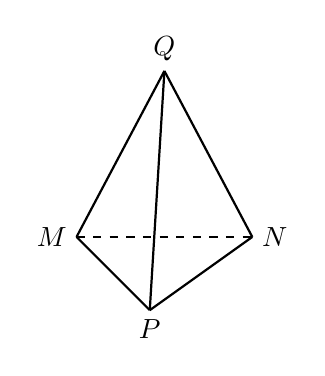
\begin{tikzpicture}[scale=0.62,>=stealth]
\draw[thick] (0,0)--(1.5,-1.5);
\draw[thick] (3.6,0)--(1.5,-1.5);
\draw[thick] (1.8,3.4)--(0,0);
\draw[thick] (1.8,3.4)--(3.6,0);
\draw[thick] (1.8,3.4)--(1.5,-1.5);
\draw[dashed] (0,0)--(3.6,0);
\node[left] at (0,0){$M$};
\node[right] at (3.6,0){$N$};
\node[below] at (1.5,-1.5){$P$};
\node[above] at (1.8,3.4){$Q$};
\end{tikzpicture}
\end{center}
  Xét tính đúng sai của các mệnh đề sau:}{%
  \y{$\overrightarrow{NM}=-\overrightarrow{MN}$.}{d}
  \y{$\overrightarrow{PM}=\overrightarrow{MQ}$.}{s}
  \y{$\overrightarrow{QN}+\overrightarrow{NP}=\overrightarrow{QP}$.}{d}
  \y{$\overrightarrow{QP}=\overrightarrow{QP}$.}{d}}

\cauDS[id=C2-B6-D01-NB-048,muc=NB,loigiai={Áp dụng quy tắc ba điểm, quy tắc hình bình hành, quy tắc hình hộp và định nghĩa hai vectơ bằng nhau. a) Đúng. b) Sai. c) Sai. d) Đúng.}]{Cho hình hộp $EFGH.E'F'G'H'$.  Xét tính đúng sai của các mệnh đề sau:}{%
  \y{$\overrightarrow{FF'}=-\overrightarrow{F'F}$.}{d}
  \y{$\overrightarrow{HG}+\overrightarrow{HE}+\overrightarrow{HH'}=\overrightarrow{HG'}$.}{s}
  \y{$\overrightarrow{FG}+\overrightarrow{FE}+\overrightarrow{FF'}=\overrightarrow{FE'}$.}{s}
  \y{$\overrightarrow{GG'}+\overrightarrow{GH}=\overrightarrow{GH'}$.}{d}}

\cauTLN[id=C2-B6-D01-NB-049,muc=NB,loigiai={Liệt kê các vectơ có hai đầu mút là đỉnh của hình thoả mãn điều kiện: có tất cả $2$ vectơ.}]{Cho hình hộp $EFGH.E'F'G'H'$ như hình vẽ.
\begin{center}
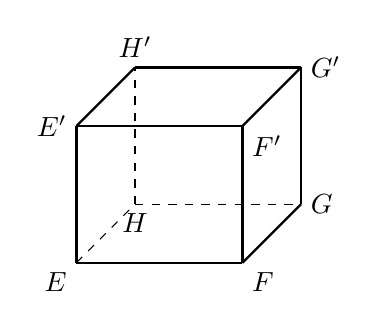
\begin{tikzpicture}[scale=0.62,>=stealth]
\draw[thick] (0,0)--(3.4,0);
\draw[thick] (3.4,0)--(4.6,1.2);
\draw[thick] (4.6,1.2)--(4.6,4.0);
\draw[thick] (0,2.8)--(3.4,2.8);
\draw[thick] (3.4,2.8)--(4.6,4.0);
\draw[thick] (4.6,4.0)--(1.2,4.0);
\draw[thick] (1.2,4.0)--(0,2.8);
\draw[thick] (0,0)--(0,2.8);
\draw[thick] (3.4,0)--(3.4,2.8);
\draw[dashed] (0,0)--(1.2,1.2);
\draw[dashed] (1.2,1.2)--(4.6,1.2);
\draw[dashed] (1.2,1.2)--(1.2,4.0);
\node[below left] at (0,0){$E$};
\node[below right] at (3.4,0){$F$};
\node[right] at (4.6,1.2){$G$};
\node[below] at (1.2,1.2){$H$};
\node[left] at (0,2.8){$E'$};
\node[below right] at (3.4,2.8){$F'$};
\node[right] at (4.6,4.0){$G'$};
\node[above] at (1.2,4.0){$H'$};
\end{tikzpicture}
\end{center}
 Có bao nhiêu vectơ khác vectơ-không có điểm đầu và điểm cuối là hai trong tám đỉnh của hình, đồng thời bằng vectơ $\overrightarrow{E'F}$ (kể cả chính $\overrightarrow{E'F}$)?}{2}

\cauTLN[id=C2-B6-D01-NB-050,muc=NB,loigiai={Liệt kê các vectơ có hai đầu mút là đỉnh của hình thoả mãn điều kiện: có tất cả $4$ vectơ.}]{Cho hình hộp $EFGH.E'F'G'H'$. Có bao nhiêu vectơ khác vectơ-không có điểm đầu và điểm cuối là hai trong tám đỉnh của hình, đồng thời bằng vectơ $\overrightarrow{E'E}$ (kể cả chính $\overrightarrow{E'E}$)?}{4}

\cauTLN[id=C2-B6-D01-NB-051,muc=NB,loigiai={Liệt kê các vectơ có hai đầu mút là đỉnh của hình thoả mãn điều kiện: có tất cả $4$ vectơ.}]{Cho hình hộp $ABCD.A'B'C'D'$. Có bao nhiêu vectơ khác vectơ-không có điểm đầu và điểm cuối là hai trong tám đỉnh của hình, đồng thời cùng phương với vectơ $\overrightarrow{D'A}$?}{4}

\cauTLN[id=C2-B6-D01-NB-052,muc=NB,loigiai={Liệt kê các vectơ có hai đầu mút là đỉnh của hình thoả mãn điều kiện: có tất cả $2$ vectơ.}]{Cho hình hộp $EFGH.E'F'G'H'$ như hình vẽ.
\begin{center}
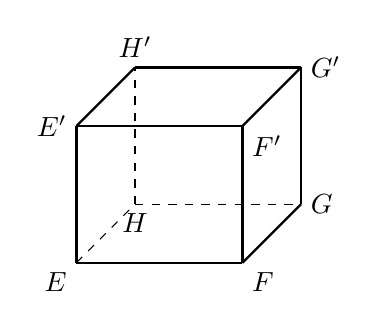
\begin{tikzpicture}[scale=0.62,>=stealth]
\draw[thick] (0,0)--(3.4,0);
\draw[thick] (3.4,0)--(4.6,1.2);
\draw[thick] (4.6,1.2)--(4.6,4.0);
\draw[thick] (0,2.8)--(3.4,2.8);
\draw[thick] (3.4,2.8)--(4.6,4.0);
\draw[thick] (4.6,4.0)--(1.2,4.0);
\draw[thick] (1.2,4.0)--(0,2.8);
\draw[thick] (0,0)--(0,2.8);
\draw[thick] (3.4,0)--(3.4,2.8);
\draw[dashed] (0,0)--(1.2,1.2);
\draw[dashed] (1.2,1.2)--(4.6,1.2);
\draw[dashed] (1.2,1.2)--(1.2,4.0);
\node[below left] at (0,0){$E$};
\node[below right] at (3.4,0){$F$};
\node[right] at (4.6,1.2){$G$};
\node[below] at (1.2,1.2){$H$};
\node[left] at (0,2.8){$E'$};
\node[below right] at (3.4,2.8){$F'$};
\node[right] at (4.6,4.0){$G'$};
\node[above] at (1.2,4.0){$H'$};
\end{tikzpicture}
\end{center}
 Có bao nhiêu vectơ khác vectơ-không có điểm đầu và điểm cuối là hai trong tám đỉnh của hình, đồng thời bằng vectơ $\overrightarrow{FG'}$ (kể cả chính $\overrightarrow{FG'}$)?}{2}

\cauTLN[id=C2-B6-D01-NB-053,muc=NB,loigiai={Liệt kê các vectơ có hai đầu mút là đỉnh của hình thoả mãn điều kiện: có tất cả $2$ vectơ.}]{Cho hình hộp $MNPQ.M'N'P'Q'$. Có bao nhiêu vectơ khác vectơ-không có điểm đầu và điểm cuối là hai trong tám đỉnh của hình, đồng thời bằng vectơ $\overrightarrow{P'M'}$ (kể cả chính $\overrightarrow{P'M'}$)?}{2}

\cauTLN[id=C2-B6-D01-NB-054,muc=NB,loigiai={Liệt kê các vectơ có hai đầu mút là đỉnh của hình thoả mãn điều kiện: có tất cả $2$ vectơ.}]{Cho hình hộp $EFGH.E'F'G'H'$. Có bao nhiêu vectơ khác vectơ-không có điểm đầu và điểm cuối là hai trong tám đỉnh của hình, đồng thời là vectơ đối của vectơ $\overrightarrow{G'E'}$?}{2}

\cauTLN[id=C2-B6-D01-NB-055,muc=NB,loigiai={Liệt kê các vectơ có hai đầu mút là đỉnh của hình thoả mãn điều kiện: có tất cả $2$ vectơ.}]{Cho hình hộp $ABCD.EFGH$ như hình vẽ.
\begin{center}
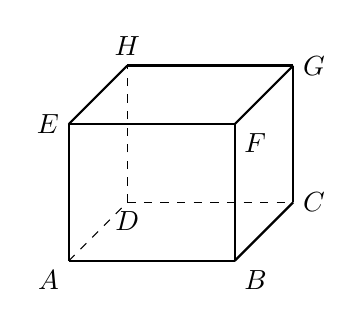
\begin{tikzpicture}[scale=0.62,>=stealth]
\draw[thick] (0,0)--(3.4,0);
\draw[thick] (3.4,0)--(4.6,1.2);
\draw[thick] (4.6,1.2)--(4.6,4.0);
\draw[thick] (0,2.8)--(3.4,2.8);
\draw[thick] (3.4,2.8)--(4.6,4.0);
\draw[thick] (4.6,4.0)--(1.2,4.0);
\draw[thick] (1.2,4.0)--(0,2.8);
\draw[thick] (0,0)--(0,2.8);
\draw[thick] (3.4,0)--(3.4,2.8);
\draw[dashed] (0,0)--(1.2,1.2);
\draw[dashed] (1.2,1.2)--(4.6,1.2);
\draw[dashed] (1.2,1.2)--(1.2,4.0);
\node[below left] at (0,0){$A$};
\node[below right] at (3.4,0){$B$};
\node[right] at (4.6,1.2){$C$};
\node[below] at (1.2,1.2){$D$};
\node[left] at (0,2.8){$E$};
\node[below right] at (3.4,2.8){$F$};
\node[right] at (4.6,4.0){$G$};
\node[above] at (1.2,4.0){$H$};
\end{tikzpicture}
\end{center}
 Có bao nhiêu vectơ khác vectơ-không có điểm đầu và điểm cuối là hai trong tám đỉnh của hình, đồng thời bằng vectơ $\overrightarrow{EG}$ (kể cả chính $\overrightarrow{EG}$)?}{2}

\cauTLN[id=C2-B6-D01-NB-056,muc=NB,loigiai={Liệt kê các vectơ có hai đầu mút là đỉnh của hình thoả mãn điều kiện: có tất cả $1$ vectơ.}]{Cho hình hộp $ABCD.A'B'C'D'$. Có bao nhiêu vectơ khác vectơ-không có điểm đầu và điểm cuối là hai trong tám đỉnh của hình, đồng thời bằng vectơ $\overrightarrow{A'C}$ (kể cả chính $\overrightarrow{A'C}$)?}{1}

\cauTLN[id=C2-B6-D01-NB-057,muc=NB,loigiai={Liệt kê các vectơ có hai đầu mút là đỉnh của hình thoả mãn điều kiện: có tất cả $2$ vectơ.}]{Cho hình hộp $ABCD.EFGH$. Có bao nhiêu vectơ khác vectơ-không có điểm đầu và điểm cuối là hai trong tám đỉnh của hình, đồng thời là vectơ đối của vectơ $\overrightarrow{FA}$?}{2}

\cauTLN[id=C2-B6-D01-NB-058,muc=NB,loigiai={Liệt kê các vectơ có hai đầu mút là đỉnh của hình thoả mãn điều kiện: có tất cả $4$ vectơ.}]{Cho hình hộp $MNPQ.M'N'P'Q'$. Có bao nhiêu vectơ khác vectơ-không có điểm đầu và điểm cuối là hai trong tám đỉnh của hình, đồng thời cùng phương với vectơ $\overrightarrow{MP}$?}{4}

\cauTLN[id=C2-B6-D01-NB-059,muc=NB,loigiai={Liệt kê các vectơ có hai đầu mút là đỉnh của hình thoả mãn điều kiện: có tất cả $8$ vectơ.}]{Cho hình hộp $EFGH.E'F'G'H'$. Có bao nhiêu vectơ khác vectơ-không có điểm đầu và điểm cuối là hai trong tám đỉnh của hình, đồng thời cùng phương với vectơ $\overrightarrow{E'F'}$?}{8}

\cauTLN[id=C2-B6-D01-NB-060,muc=NB,loigiai={Liệt kê các vectơ có hai đầu mút là đỉnh của hình thoả mãn điều kiện: có tất cả $4$ vectơ.}]{Cho hình hộp $MNPQ.M'N'P'Q'$ như hình vẽ.
\begin{center}
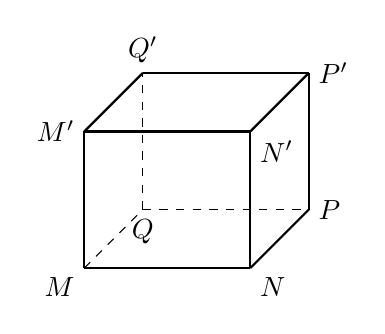
\begin{tikzpicture}[scale=0.62,>=stealth]
\draw[thick] (0,0)--(3.4,0);
\draw[thick] (3.4,0)--(4.6,1.2);
\draw[thick] (4.6,1.2)--(4.6,4.0);
\draw[thick] (0,2.8)--(3.4,2.8);
\draw[thick] (3.4,2.8)--(4.6,4.0);
\draw[thick] (4.6,4.0)--(1.2,4.0);
\draw[thick] (1.2,4.0)--(0,2.8);
\draw[thick] (0,0)--(0,2.8);
\draw[thick] (3.4,0)--(3.4,2.8);
\draw[dashed] (0,0)--(1.2,1.2);
\draw[dashed] (1.2,1.2)--(4.6,1.2);
\draw[dashed] (1.2,1.2)--(1.2,4.0);
\node[below left] at (0,0){$M$};
\node[below right] at (3.4,0){$N$};
\node[right] at (4.6,1.2){$P$};
\node[below] at (1.2,1.2){$Q$};
\node[left] at (0,2.8){$M'$};
\node[below right] at (3.4,2.8){$N'$};
\node[right] at (4.6,4.0){$P'$};
\node[above] at (1.2,4.0){$Q'$};
\end{tikzpicture}
\end{center}
 Có bao nhiêu vectơ khác vectơ-không có điểm đầu và điểm cuối là hai trong tám đỉnh của hình, đồng thời cùng phương với vectơ $\overrightarrow{P'Q}$?}{4}

\cauTN[id=C2-B6-D01-TH-001,muc=TH,loigiai={Ta có $\overrightarrow{DB}=\overrightarrow{AB}-\overrightarrow{AD}$ (phân tích theo các cạnh xuất phát từ cùng một đỉnh, dùng quy tắc ba điểm, quy tắc hình bình hành). Do đó $\overrightarrow{DB}=\vec{a}-\vec{c}$.}]{Cho tứ diện $ABCD$ như hình vẽ.
\begin{center}
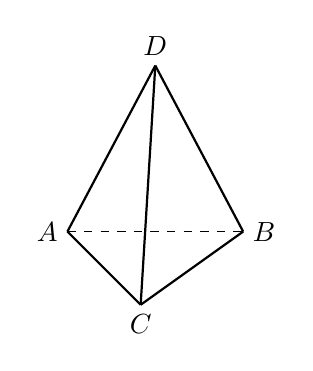
\begin{tikzpicture}[scale=0.62,>=stealth]
\draw[thick] (0,0)--(1.5,-1.5);
\draw[thick] (3.6,0)--(1.5,-1.5);
\draw[thick] (1.8,3.4)--(0,0);
\draw[thick] (1.8,3.4)--(3.6,0);
\draw[thick] (1.8,3.4)--(1.5,-1.5);
\draw[dashed] (0,0)--(3.6,0);
\node[left] at (0,0){$A$};
\node[right] at (3.6,0){$B$};
\node[below] at (1.5,-1.5){$C$};
\node[above] at (1.8,3.4){$D$};
\end{tikzpicture}
\end{center}
 Đặt $\vec{a}=\overrightarrow{AB}$, $\vec{b}=\overrightarrow{AC}$, $\vec{c}=\overrightarrow{AD}$. Biểu diễn vectơ $\overrightarrow{DB}$ theo ba vectơ $\vec{a}$, $\vec{b}$, $\vec{c}$ ta được}
  {$\vec{a}-\vec{c}$.}
  {$\vec{a}+\vec{c}$.}{$\vec{a}-2\vec{b}-\vec{c}$.}{$\vec{a}+\vec{b}-\vec{c}$.}

\cauTN[id=C2-B6-D01-TH-002,muc=TH,loigiai={Ta có $\overrightarrow{PQ}=\overrightarrow{MQ}-\overrightarrow{MP}$ (phân tích theo các cạnh xuất phát từ cùng một đỉnh, dùng quy tắc ba điểm, quy tắc hình bình hành). Do đó $\overrightarrow{PQ}=-\vec{b}+\vec{c}$.}]{Cho tứ diện $MNPQ$. Đặt $\vec{a}=\overrightarrow{MN}$, $\vec{b}=\overrightarrow{MP}$, $\vec{c}=\overrightarrow{MQ}$. Biểu diễn vectơ $\overrightarrow{PQ}$ theo ba vectơ $\vec{a}$, $\vec{b}$, $\vec{c}$ ta được}
  {$-\vec{b}+\vec{c}$.}
  {$2\vec{a}-\vec{b}+\vec{c}$.}{$-\vec{a}+\vec{c}$.}{$\vec{a}-\vec{b}$.}

\cauTN[id=C2-B6-D01-TH-003,muc=TH,loigiai={Ta có $\overrightarrow{D'B}=\overrightarrow{AB}-\overrightarrow{AD'}$ (phân tích theo các cạnh xuất phát từ cùng một đỉnh, dùng quy tắc ba điểm, quy tắc hình bình hành). Do đó $\overrightarrow{D'B}=\vec{a}-\vec{b}-\vec{c}$.}]{Cho hình hộp $ABCD.A'B'C'D'$. Đặt $\vec{a}=\overrightarrow{AB}$, $\vec{b}=\overrightarrow{AD}$, $\vec{c}=\overrightarrow{AA'}$. Biểu diễn vectơ $\overrightarrow{D'B}$ theo ba vectơ $\vec{a}$, $\vec{b}$, $\vec{c}$ ta được}
  {$\vec{a}-\vec{b}-\vec{c}$.}
  {$-\vec{a}-\vec{b}-\vec{c}$.}{$\vec{a}-2\vec{b}-\vec{c}$.}{$\vec{a}-\vec{b}$.}

\cauTN[id=C2-B6-D01-TH-004,muc=TH,loigiai={Ta có $\overrightarrow{C'D}=\overrightarrow{AD}-\overrightarrow{AC'}$ (phân tích theo các cạnh xuất phát từ cùng một đỉnh, dùng quy tắc ba điểm, quy tắc hình bình hành). Do đó $\overrightarrow{C'D}=-\vec{a}-\vec{c}$.}]{Cho hình hộp $ABCD.A'B'C'D'$. Đặt $\vec{a}=\overrightarrow{AB}$, $\vec{b}=\overrightarrow{AD}$, $\vec{c}=\overrightarrow{AA'}$. Biểu diễn vectơ $\overrightarrow{C'D}$ theo ba vectơ $\vec{a}$, $\vec{b}$, $\vec{c}$ ta được}
  {$-\vec{a}-\vec{c}$.}
  {$-\vec{a}+2\vec{b}-\vec{c}$.}{$-\vec{a}+\vec{c}$.}{$-2\vec{a}-\vec{c}$.}

\cauTN[id=C2-B6-D01-TH-005,muc=TH,loigiai={Ta có $\overrightarrow{PM}=\overrightarrow{MM}-\overrightarrow{MP}$ (phân tích theo các cạnh xuất phát từ cùng một đỉnh, dùng quy tắc ba điểm, quy tắc hình bình hành). Do đó $\overrightarrow{PM}=-\vec{a}-\vec{b}$.}]{Cho hình hộp $MNPQ.M'N'P'Q'$. Đặt $\vec{a}=\overrightarrow{MN}$, $\vec{b}=\overrightarrow{MQ}$, $\vec{c}=\overrightarrow{MM'}$. Biểu diễn vectơ $\overrightarrow{PM}$ theo ba vectơ $\vec{a}$, $\vec{b}$, $\vec{c}$ ta được}
  {$-\vec{a}-\vec{b}$.}
  {$-\vec{a}+\vec{b}$.}{$-\vec{a}-2\vec{b}$.}{$-\vec{a}$.}

\cauTN[id=C2-B6-D01-TH-006,muc=TH,loigiai={Ta có $\overrightarrow{M'N}=\overrightarrow{MN}-\overrightarrow{MM'}$ (phân tích theo các cạnh xuất phát từ cùng một đỉnh, dùng quy tắc ba điểm, quy tắc hình bình hành). Do đó $\overrightarrow{M'N}=\vec{a}-\vec{c}$.}]{Cho hình hộp $MNPQ.M'N'P'Q'$. Đặt $\vec{a}=\overrightarrow{MN}$, $\vec{b}=\overrightarrow{MQ}$, $\vec{c}=\overrightarrow{MM'}$. Biểu diễn vectơ $\overrightarrow{M'N}$ theo ba vectơ $\vec{a}$, $\vec{b}$, $\vec{c}$ ta được}
  {$\vec{a}-\vec{c}$.}
  {$\vec{b}-\vec{c}$.}{$\vec{a}$.}{$-\vec{c}$.}

\cauTN[id=C2-B6-D01-TH-007,muc=TH,loigiai={Ta có $\overrightarrow{EG}=\overrightarrow{EG}-\overrightarrow{EE}$ (phân tích theo các cạnh xuất phát từ cùng một đỉnh, dùng quy tắc ba điểm, quy tắc hình bình hành). Do đó $\overrightarrow{EG}=\vec{a}+\vec{b}$.}]{Cho hình hộp $EFGH.E'F'G'H'$ như hình vẽ.
\begin{center}
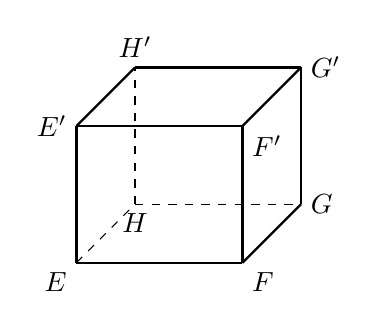
\begin{tikzpicture}[scale=0.62,>=stealth]
\draw[thick] (0,0)--(3.4,0);
\draw[thick] (3.4,0)--(4.6,1.2);
\draw[thick] (4.6,1.2)--(4.6,4.0);
\draw[thick] (0,2.8)--(3.4,2.8);
\draw[thick] (3.4,2.8)--(4.6,4.0);
\draw[thick] (4.6,4.0)--(1.2,4.0);
\draw[thick] (1.2,4.0)--(0,2.8);
\draw[thick] (0,0)--(0,2.8);
\draw[thick] (3.4,0)--(3.4,2.8);
\draw[dashed] (0,0)--(1.2,1.2);
\draw[dashed] (1.2,1.2)--(4.6,1.2);
\draw[dashed] (1.2,1.2)--(1.2,4.0);
\node[below left] at (0,0){$E$};
\node[below right] at (3.4,0){$F$};
\node[right] at (4.6,1.2){$G$};
\node[below] at (1.2,1.2){$H$};
\node[left] at (0,2.8){$E'$};
\node[below right] at (3.4,2.8){$F'$};
\node[right] at (4.6,4.0){$G'$};
\node[above] at (1.2,4.0){$H'$};
\end{tikzpicture}
\end{center}
 Đặt $\vec{a}=\overrightarrow{EF}$, $\vec{b}=\overrightarrow{EH}$, $\vec{c}=\overrightarrow{EE'}$. Biểu diễn vectơ $\overrightarrow{EG}$ theo ba vectơ $\vec{a}$, $\vec{b}$, $\vec{c}$ ta được}
  {$\vec{a}+\vec{b}$.}
  {$\vec{a}$.}{$\vec{a}+\vec{c}$.}{$\vec{a}+2\vec{b}$.}

\cauTN[id=C2-B6-D01-TH-008,muc=TH,loigiai={Ta có $\overrightarrow{A'D}=\overrightarrow{AD}-\overrightarrow{AA'}$ (phân tích theo các cạnh xuất phát từ cùng một đỉnh, dùng quy tắc ba điểm, quy tắc hình bình hành). Do đó $\overrightarrow{A'D}=\vec{b}-\vec{c}$.}]{Cho hình hộp $ABCD.A'B'C'D'$. Đặt $\vec{a}=\overrightarrow{AB}$, $\vec{b}=\overrightarrow{AD}$, $\vec{c}=\overrightarrow{AA'}$. Biểu diễn vectơ $\overrightarrow{A'D}$ theo ba vectơ $\vec{a}$, $\vec{b}$, $\vec{c}$ ta được}
  {$\vec{b}-\vec{c}$.}
  {$-\vec{b}-\vec{c}$.}{$\vec{b}+\vec{c}$.}{$-\vec{c}$.}

\cauTN[id=C2-B6-D01-TH-009,muc=TH,loigiai={Ta có $\overrightarrow{DG}=\overrightarrow{AG}-\overrightarrow{AD}$ (phân tích theo các cạnh xuất phát từ cùng một đỉnh, dùng quy tắc ba điểm, quy tắc hình bình hành). Do đó $\overrightarrow{DG}=\vec{a}+\vec{c}$.}]{Cho hình hộp $ABCD.EFGH$. Đặt $\vec{a}=\overrightarrow{AB}$, $\vec{b}=\overrightarrow{AD}$, $\vec{c}=\overrightarrow{AE}$. Biểu diễn vectơ $\overrightarrow{DG}$ theo ba vectơ $\vec{a}$, $\vec{b}$, $\vec{c}$ ta được}
  {$\vec{a}+\vec{c}$.}
  {$-\vec{a}+\vec{c}$.}{$\vec{c}$.}{$\vec{a}+3\vec{c}$.}

\cauTN[id=C2-B6-D01-TH-010,muc=TH,loigiai={Ta có $\overrightarrow{CA}=\overrightarrow{AA}-\overrightarrow{AC}$ (phân tích theo các cạnh xuất phát từ cùng một đỉnh, dùng quy tắc ba điểm, quy tắc hình bình hành). Do đó $\overrightarrow{CA}=-\vec{a}-\vec{b}$.}]{Cho hình chóp $O.ABCD$ có đáy $ABCD$ là hình bình hành như hình vẽ.
\begin{center}
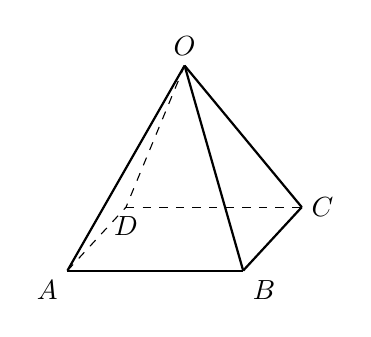
\begin{tikzpicture}[scale=0.62,>=stealth]
\draw[thick] (0,0)--(3.6,0);
\draw[thick] (3.6,0)--(4.8,1.3);
\draw[thick] (2.4,4.2)--(0,0);
\draw[thick] (2.4,4.2)--(3.6,0);
\draw[thick] (2.4,4.2)--(4.8,1.3);
\draw[dashed] (0,0)--(1.2,1.3);
\draw[dashed] (1.2,1.3)--(4.8,1.3);
\draw[dashed] (2.4,4.2)--(1.2,1.3);
\node[below left] at (0,0){$A$};
\node[below right] at (3.6,0){$B$};
\node[right] at (4.8,1.3){$C$};
\node[below] at (1.2,1.3){$D$};
\node[above] at (2.4,4.2){$O$};
\end{tikzpicture}
\end{center}
 Đặt $\vec{a}=\overrightarrow{AB}$, $\vec{b}=\overrightarrow{AD}$, $\vec{c}=\overrightarrow{AO}$. Biểu diễn vectơ $\overrightarrow{CA}$ theo ba vectơ $\vec{a}$, $\vec{b}$, $\vec{c}$ ta được}
  {$-\vec{a}-\vec{b}$.}
  {$-\vec{a}-\vec{b}-2\vec{c}$.}{$-\vec{b}$.}{$-\vec{a}-3\vec{b}$.}

\cauTN[id=C2-B6-D01-TH-011,muc=TH,loigiai={Ta có $\overrightarrow{Q'N}=\overrightarrow{MN}-\overrightarrow{MQ'}$ (phân tích theo các cạnh xuất phát từ cùng một đỉnh, dùng quy tắc ba điểm, quy tắc hình bình hành). Do đó $\overrightarrow{Q'N}=\vec{a}-\vec{b}-\vec{c}$.}]{Cho hình hộp $MNPQ.M'N'P'Q'$. Đặt $\vec{a}=\overrightarrow{MN}$, $\vec{b}=\overrightarrow{MQ}$, $\vec{c}=\overrightarrow{MM'}$. Biểu diễn vectơ $\overrightarrow{Q'N}$ theo ba vectơ $\vec{a}$, $\vec{b}$, $\vec{c}$ ta được}
  {$\vec{a}-\vec{b}-\vec{c}$.}
  {$-\vec{a}+\vec{b}-\vec{c}$.}{$\vec{a}-\vec{b}+\vec{c}$.}{$\vec{a}-\vec{c}$.}

\cauTN[id=C2-B6-D01-TH-012,muc=TH,loigiai={Ta có $\overrightarrow{N'Q'}=\overrightarrow{MQ'}-\overrightarrow{MN'}$ (phân tích theo các cạnh xuất phát từ cùng một đỉnh, dùng quy tắc ba điểm, quy tắc hình bình hành). Do đó $\overrightarrow{N'Q'}=-\vec{a}+\vec{b}$.}]{Cho hình hộp $MNPQ.M'N'P'Q'$ như hình vẽ.
\begin{center}
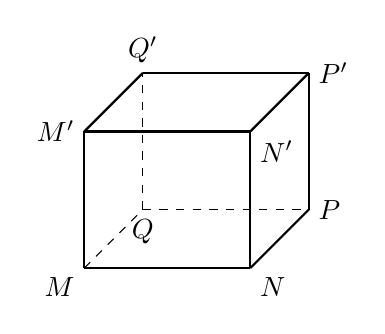
\begin{tikzpicture}[scale=0.62,>=stealth]
\draw[thick] (0,0)--(3.4,0);
\draw[thick] (3.4,0)--(4.6,1.2);
\draw[thick] (4.6,1.2)--(4.6,4.0);
\draw[thick] (0,2.8)--(3.4,2.8);
\draw[thick] (3.4,2.8)--(4.6,4.0);
\draw[thick] (4.6,4.0)--(1.2,4.0);
\draw[thick] (1.2,4.0)--(0,2.8);
\draw[thick] (0,0)--(0,2.8);
\draw[thick] (3.4,0)--(3.4,2.8);
\draw[dashed] (0,0)--(1.2,1.2);
\draw[dashed] (1.2,1.2)--(4.6,1.2);
\draw[dashed] (1.2,1.2)--(1.2,4.0);
\node[below left] at (0,0){$M$};
\node[below right] at (3.4,0){$N$};
\node[right] at (4.6,1.2){$P$};
\node[below] at (1.2,1.2){$Q$};
\node[left] at (0,2.8){$M'$};
\node[below right] at (3.4,2.8){$N'$};
\node[right] at (4.6,4.0){$P'$};
\node[above] at (1.2,4.0){$Q'$};
\end{tikzpicture}
\end{center}
 Đặt $\vec{a}=\overrightarrow{MN}$, $\vec{b}=\overrightarrow{MQ}$, $\vec{c}=\overrightarrow{MM'}$. Biểu diễn vectơ $\overrightarrow{N'Q'}$ theo ba vectơ $\vec{a}$, $\vec{b}$, $\vec{c}$ ta được}
  {$-\vec{a}+\vec{b}$.}
  {$-\vec{a}+\vec{b}-\vec{c}$.}{$-\vec{a}-\vec{b}$.}{$-\vec{a}+\vec{b}+2\vec{c}$.}

\cauTN[id=C2-B6-D01-TH-013,muc=TH,loigiai={Dùng các quy tắc cộng vectơ và tính chất hai vectơ bằng nhau (các cạnh song song bằng nhau trong hình) ta có $\overrightarrow{D'D}+\overrightarrow{D'C'}+\overrightarrow{BA}+\overrightarrow{B'D'}=\overrightarrow{B'D}$.}]{Cho hình hộp $ABCD.A'B'C'D'$. Tổng $\overrightarrow{D'D}+\overrightarrow{D'C'}+\overrightarrow{BA}+\overrightarrow{B'D'}$ bằng vectơ nào sau đây?}
  {$\overrightarrow{B'D}$.}
  {$\overrightarrow{DB'}$.}{$\overrightarrow{A'C'}$.}{$\overrightarrow{CD}$.}

\cauTN[id=C2-B6-D01-TH-014,muc=TH,loigiai={Dùng các quy tắc cộng vectơ và tính chất hai vectơ bằng nhau (các cạnh song song bằng nhau trong hình) ta có $\overrightarrow{B'C}+\overrightarrow{AB'}+\overrightarrow{DB'}+\overrightarrow{B'D}=\overrightarrow{AC}$.}]{Cho hình hộp $ABCD.A'B'C'D'$. Tổng $\overrightarrow{B'C}+\overrightarrow{AB'}+\overrightarrow{DB'}+\overrightarrow{B'D}$ bằng vectơ nào sau đây?}
  {$\overrightarrow{AC}$.}
  {$\overrightarrow{CA}$.}{$\overrightarrow{CD'}$.}{$\overrightarrow{D'D}$.}

\cauTN[id=C2-B6-D01-TH-015,muc=TH,loigiai={Dùng các quy tắc cộng vectơ và tính chất hai vectơ bằng nhau (các cạnh song song bằng nhau trong hình) ta có $\overrightarrow{FH}+\overrightarrow{DC}+\overrightarrow{HA}=\overrightarrow{HD}$.}]{Cho hình hộp $ABCD.EFGH$. Tổng $\overrightarrow{FH}+\overrightarrow{DC}+\overrightarrow{HA}$ bằng vectơ nào sau đây?}
  {$\overrightarrow{HD}$.}
  {$\overrightarrow{DH}$.}{$\overrightarrow{GD}$.}{$\overrightarrow{BD}$.}

\cauTN[id=C2-B6-D01-TH-016,muc=TH,loigiai={Dùng các quy tắc cộng vectơ và tính chất hai vectơ bằng nhau (các cạnh song song bằng nhau trong hình) ta có $\overrightarrow{DD'}+\overrightarrow{BA}+\overrightarrow{D'C'}+\overrightarrow{A'D'}=\overrightarrow{AD'}$.}]{Cho hình hộp $ABCD.A'B'C'D'$. Tổng $\overrightarrow{DD'}+\overrightarrow{BA}+\overrightarrow{D'C'}+\overrightarrow{A'D'}$ bằng vectơ nào sau đây?}
  {$\overrightarrow{AD'}$.}
  {$\overrightarrow{D'A}$.}{$\overrightarrow{BB'}$.}{$\overrightarrow{DA'}$.}

\cauTN[id=C2-B6-D01-TH-017,muc=TH,loigiai={Dùng các quy tắc cộng vectơ và tính chất hai vectơ bằng nhau (các cạnh song song bằng nhau trong hình) ta có $\overrightarrow{AF}+\overrightarrow{EH}+\overrightarrow{DC}+\overrightarrow{GD}=\overrightarrow{EG}$.}]{Cho hình hộp $ABCD.EFGH$. Tổng $\overrightarrow{AF}+\overrightarrow{EH}+\overrightarrow{DC}+\overrightarrow{GD}$ bằng vectơ nào sau đây?}
  {$\overrightarrow{EG}$.}
  {$\overrightarrow{GE}$.}{$\overrightarrow{GA}$.}{$\overrightarrow{CF}$.}

\cauTN[id=C2-B6-D01-TH-018,muc=TH,loigiai={Dùng các quy tắc cộng vectơ và tính chất hai vectơ bằng nhau (các cạnh song song bằng nhau trong hình) ta có $\overrightarrow{PM}+\overrightarrow{NP}+\overrightarrow{SP}=\overrightarrow{SQ}$.}]{Cho hình chóp $S.MNPQ$ có đáy $MNPQ$ là hình bình hành. Tổng $\overrightarrow{PM}+\overrightarrow{NP}+\overrightarrow{SP}$ bằng vectơ nào sau đây?}
  {$\overrightarrow{SQ}$.}
  {$\overrightarrow{QS}$.}{$\overrightarrow{MS}$.}{$\overrightarrow{SN}$.}

\cauTN[id=C2-B6-D01-TH-019,muc=TH,loigiai={Dùng các quy tắc cộng vectơ và tính chất hai vectơ bằng nhau (các cạnh song song bằng nhau trong hình) ta có $\overrightarrow{BC}+\overrightarrow{FE}+\overrightarrow{FB}=\overrightarrow{FD}$.}]{Cho hình hộp $ABCD.EFGH$. Tổng $\overrightarrow{BC}+\overrightarrow{FE}+\overrightarrow{FB}$ bằng vectơ nào sau đây?}
  {$\overrightarrow{FD}$.}
  {$\overrightarrow{DF}$.}{$\overrightarrow{EA}$.}{$\overrightarrow{FH}$.}

\cauTN[id=C2-B6-D01-TH-020,muc=TH,loigiai={Dùng các quy tắc cộng vectơ và tính chất hai vectơ bằng nhau (các cạnh song song bằng nhau trong hình) ta có $\overrightarrow{AD}+\overrightarrow{DB}+\overrightarrow{B'C}=\overrightarrow{A'C}$.}]{Cho hình hộp $ABCD.A'B'C'D'$ như hình vẽ.
\begin{center}
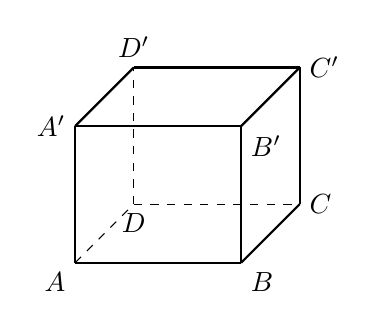
\begin{tikzpicture}[scale=0.62,>=stealth]
\draw[thick] (0,0)--(3.4,0);
\draw[thick] (3.4,0)--(4.6,1.2);
\draw[thick] (4.6,1.2)--(4.6,4.0);
\draw[thick] (0,2.8)--(3.4,2.8);
\draw[thick] (3.4,2.8)--(4.6,4.0);
\draw[thick] (4.6,4.0)--(1.2,4.0);
\draw[thick] (1.2,4.0)--(0,2.8);
\draw[thick] (0,0)--(0,2.8);
\draw[thick] (3.4,0)--(3.4,2.8);
\draw[dashed] (0,0)--(1.2,1.2);
\draw[dashed] (1.2,1.2)--(4.6,1.2);
\draw[dashed] (1.2,1.2)--(1.2,4.0);
\node[below left] at (0,0){$A$};
\node[below right] at (3.4,0){$B$};
\node[right] at (4.6,1.2){$C$};
\node[below] at (1.2,1.2){$D$};
\node[left] at (0,2.8){$A'$};
\node[below right] at (3.4,2.8){$B'$};
\node[right] at (4.6,4.0){$C'$};
\node[above] at (1.2,4.0){$D'$};
\end{tikzpicture}
\end{center}
 Tổng $\overrightarrow{AD}+\overrightarrow{DB}+\overrightarrow{B'C}$ bằng vectơ nào sau đây?}
  {$\overrightarrow{A'C}$.}
  {$\overrightarrow{CA'}$.}{$\overrightarrow{DB}$.}{$\overrightarrow{A'B}$.}

\cauTN[id=C2-B6-D01-TH-021,muc=TH,loigiai={Dùng các quy tắc cộng vectơ và tính chất hai vectơ bằng nhau (các cạnh song song bằng nhau trong hình) ta có $\overrightarrow{QP}+\overrightarrow{MN}+\overrightarrow{P'Q}=\overrightarrow{Q'P}$.}]{Cho hình hộp $MNPQ.M'N'P'Q'$. Tổng $\overrightarrow{QP}+\overrightarrow{MN}+\overrightarrow{P'Q}$ bằng vectơ nào sau đây?}
  {$\overrightarrow{Q'P}$.}
  {$\overrightarrow{PQ'}$.}{$\overrightarrow{MN}$.}{$\overrightarrow{PN'}$.}

\cauTN[id=C2-B6-D01-TH-022,muc=TH,loigiai={Dùng các quy tắc cộng vectơ và tính chất hai vectơ bằng nhau (các cạnh song song bằng nhau trong hình) ta có $\overrightarrow{GH'}+\overrightarrow{HE}+\overrightarrow{F'G}=\overrightarrow{FE}$.}]{Cho hình hộp $EFGH.E'F'G'H'$. Tổng $\overrightarrow{GH'}+\overrightarrow{HE}+\overrightarrow{F'G}$ bằng vectơ nào sau đây?}
  {$\overrightarrow{FE}$.}
  {$\overrightarrow{EF}$.}{$\overrightarrow{GG'}$.}{$\overrightarrow{FE'}$.}

\cauTN[id=C2-B6-D01-TH-023,muc=TH,loigiai={Dùng các quy tắc cộng vectơ và tính chất hai vectơ bằng nhau (các cạnh song song bằng nhau trong hình) ta có $\overrightarrow{BC}+\overrightarrow{GE}+\overrightarrow{AD}=\overrightarrow{BD}$.}]{Cho hình hộp $ABCD.EFGH$. Tổng $\overrightarrow{BC}+\overrightarrow{GE}+\overrightarrow{AD}$ bằng vectơ nào sau đây?}
  {$\overrightarrow{BD}$.}
  {$\overrightarrow{DB}$.}{$\overrightarrow{GH}$.}{$\overrightarrow{GA}$.}

\cauTN[id=C2-B6-D01-TH-024,muc=TH,loigiai={Dùng các quy tắc cộng vectơ và tính chất hai vectơ bằng nhau (các cạnh song song bằng nhau trong hình) ta có $\overrightarrow{CA}+\overrightarrow{BS}+\overrightarrow{AB}=\overrightarrow{CS}$.}]{Cho hình chóp $S.ABCD$ có đáy $ABCD$ là hình bình hành như hình vẽ.
\begin{center}
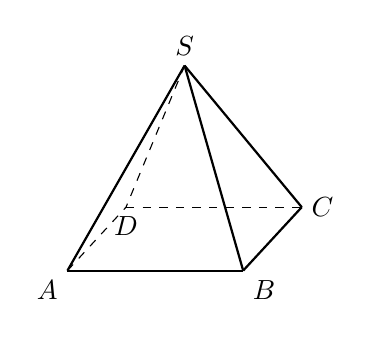
\begin{tikzpicture}[scale=0.62,>=stealth]
\draw[thick] (0,0)--(3.6,0);
\draw[thick] (3.6,0)--(4.8,1.3);
\draw[thick] (2.4,4.2)--(0,0);
\draw[thick] (2.4,4.2)--(3.6,0);
\draw[thick] (2.4,4.2)--(4.8,1.3);
\draw[dashed] (0,0)--(1.2,1.3);
\draw[dashed] (1.2,1.3)--(4.8,1.3);
\draw[dashed] (2.4,4.2)--(1.2,1.3);
\node[below left] at (0,0){$A$};
\node[below right] at (3.6,0){$B$};
\node[right] at (4.8,1.3){$C$};
\node[below] at (1.2,1.3){$D$};
\node[above] at (2.4,4.2){$S$};
\end{tikzpicture}
\end{center}
 Tổng $\overrightarrow{CA}+\overrightarrow{BS}+\overrightarrow{AB}$ bằng vectơ nào sau đây?}
  {$\overrightarrow{CS}$.}
  {$\overrightarrow{SC}$.}{$\overrightarrow{BA}$.}{$\overrightarrow{AB}$.}

\cauTN[id=C2-B6-D01-TH-025,muc=TH,loigiai={Do $I$ là trung điểm nên $\overrightarrow{MD}+\overrightarrow{MB}=2\,\overrightarrow{MI}$, suy ra $k=2$.}]{Cho hình chóp $O.ABCD$ có đáy $ABCD$ là hình bình hành như hình vẽ.
\begin{center}
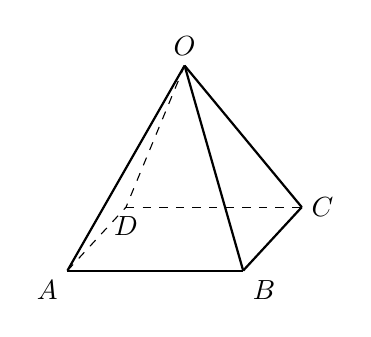
\begin{tikzpicture}[scale=0.62,>=stealth]
\draw[thick] (0,0)--(3.6,0);
\draw[thick] (3.6,0)--(4.8,1.3);
\draw[thick] (2.4,4.2)--(0,0);
\draw[thick] (2.4,4.2)--(3.6,0);
\draw[thick] (2.4,4.2)--(4.8,1.3);
\draw[dashed] (0,0)--(1.2,1.3);
\draw[dashed] (1.2,1.3)--(4.8,1.3);
\draw[dashed] (2.4,4.2)--(1.2,1.3);
\node[below left] at (0,0){$A$};
\node[below right] at (3.6,0){$B$};
\node[right] at (4.8,1.3){$C$};
\node[below] at (1.2,1.3){$D$};
\node[above] at (2.4,4.2){$O$};
\end{tikzpicture}
\end{center}
Gọi $I$ là trung điểm của đoạn thẳng $DB$.  Với điểm $M$ bất kì, ta có $\overrightarrow{MD}+\overrightarrow{MB}=k\,\overrightarrow{MI}$. Giá trị của $k$ là}
  {$2$.}
  {$1$.}{$3$.}{$4$.}

\cauTN[id=C2-B6-D01-TH-026,muc=TH,loigiai={Do $G$ là trọng tâm tam giác nên $\overrightarrow{MS}+\overrightarrow{MC}+\overrightarrow{MD}=3\,\overrightarrow{MG}$, suy ra $k=3$.}]{Cho hình chóp $S.ABCD$ có đáy $ABCD$ là hình bình hành như hình vẽ.
\begin{center}
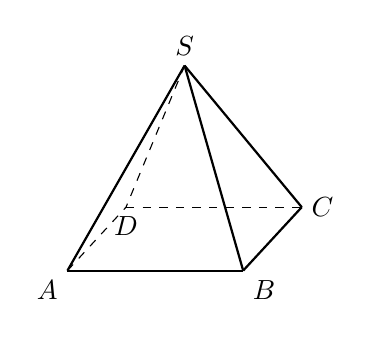
\begin{tikzpicture}[scale=0.62,>=stealth]
\draw[thick] (0,0)--(3.6,0);
\draw[thick] (3.6,0)--(4.8,1.3);
\draw[thick] (2.4,4.2)--(0,0);
\draw[thick] (2.4,4.2)--(3.6,0);
\draw[thick] (2.4,4.2)--(4.8,1.3);
\draw[dashed] (0,0)--(1.2,1.3);
\draw[dashed] (1.2,1.3)--(4.8,1.3);
\draw[dashed] (2.4,4.2)--(1.2,1.3);
\node[below left] at (0,0){$A$};
\node[below right] at (3.6,0){$B$};
\node[right] at (4.8,1.3){$C$};
\node[below] at (1.2,1.3){$D$};
\node[above] at (2.4,4.2){$S$};
\end{tikzpicture}
\end{center}
Gọi $G$ là trọng tâm của tam giác $SCD$.  Với điểm $M$ bất kì, ta có $\overrightarrow{MS}+\overrightarrow{MC}+\overrightarrow{MD}=k\,\overrightarrow{MG}$. Giá trị của $k$ là}
  {$3$.}
  {$2$.}{$4$.}{$6$.}

\cauTN[id=C2-B6-D01-TH-027,muc=TH,loigiai={Do $O$ là giao điểm hai đường chéo (trung điểm mỗi đường) nên $\overrightarrow{MA}+\overrightarrow{MC}=2\,\overrightarrow{MO}$, suy ra $k=2$.}]{Cho hình chóp $S.ABCD$ có đáy $ABCD$ là hình bình hành. Gọi $O$ là giao điểm của hai đường chéo của đáy. Với điểm $M$ bất kì, ta có $\overrightarrow{MA}+\overrightarrow{MC}=k\,\overrightarrow{MO}$. Giá trị của $k$ là}
  {$2$.}
  {$1$.}{$3$.}{$4$.}

\cauTN[id=C2-B6-D01-TH-028,muc=TH,loigiai={Do $G$ là trọng tâm tam giác nên $\overrightarrow{OS}+\overrightarrow{ON}+\overrightarrow{OP}=3\,\overrightarrow{OG}$, suy ra $k=3$.}]{Cho hình chóp $S.MNPQ$ có đáy $MNPQ$ là hình bình hành. Gọi $G$ là trọng tâm của tam giác $SNP$. Với điểm $O$ bất kì, ta có $\overrightarrow{OS}+\overrightarrow{ON}+\overrightarrow{OP}=k\,\overrightarrow{OG}$. Giá trị của $k$ là}
  {$3$.}
  {$2$.}{$4$.}{$6$.}

\cauTN[id=C2-B6-D01-TH-029,muc=TH,loigiai={Do $G$ là trọng tâm tứ diện nên $\overrightarrow{OM}+\overrightarrow{ON}+\overrightarrow{OP}+\overrightarrow{OQ}=4\,\overrightarrow{OG}$, suy ra $k=4$.}]{Cho tứ diện $MNPQ$ như hình vẽ.
\begin{center}
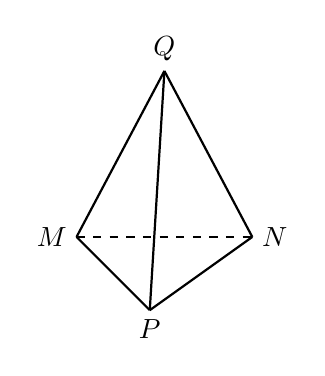
\begin{tikzpicture}[scale=0.62,>=stealth]
\draw[thick] (0,0)--(1.5,-1.5);
\draw[thick] (3.6,0)--(1.5,-1.5);
\draw[thick] (1.8,3.4)--(0,0);
\draw[thick] (1.8,3.4)--(3.6,0);
\draw[thick] (1.8,3.4)--(1.5,-1.5);
\draw[dashed] (0,0)--(3.6,0);
\node[left] at (0,0){$M$};
\node[right] at (3.6,0){$N$};
\node[below] at (1.5,-1.5){$P$};
\node[above] at (1.8,3.4){$Q$};
\end{tikzpicture}
\end{center}
Gọi $G$ là trọng tâm của tứ diện $MNPQ$.  Với điểm $O$ bất kì, ta có $\overrightarrow{OM}+\overrightarrow{ON}+\overrightarrow{OP}+\overrightarrow{OQ}=k\,\overrightarrow{OG}$. Giá trị của $k$ là}
  {$4$.}
  {$3$.}{$5$.}{$8$.}

\cauTN[id=C2-B6-D01-TH-030,muc=TH,loigiai={Do $I$ là trung điểm nên $\overrightarrow{MD}+\overrightarrow{MB}=2\,\overrightarrow{MI}$, suy ra $k=2$.}]{Cho tứ diện $ABCD$ như hình vẽ.
\begin{center}
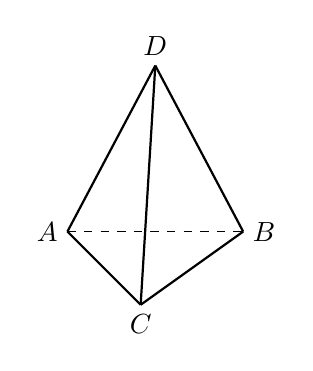
\begin{tikzpicture}[scale=0.62,>=stealth]
\draw[thick] (0,0)--(1.5,-1.5);
\draw[thick] (3.6,0)--(1.5,-1.5);
\draw[thick] (1.8,3.4)--(0,0);
\draw[thick] (1.8,3.4)--(3.6,0);
\draw[thick] (1.8,3.4)--(1.5,-1.5);
\draw[dashed] (0,0)--(3.6,0);
\node[left] at (0,0){$A$};
\node[right] at (3.6,0){$B$};
\node[below] at (1.5,-1.5){$C$};
\node[above] at (1.8,3.4){$D$};
\end{tikzpicture}
\end{center}
Gọi $I$ là trung điểm của đoạn thẳng $DB$.  Với điểm $M$ bất kì, ta có $\overrightarrow{MD}+\overrightarrow{MB}=k\,\overrightarrow{MI}$. Giá trị của $k$ là}
  {$2$.}
  {$1$.}{$3$.}{$4$.}

\cauTN[id=C2-B6-D01-TH-031,muc=TH,loigiai={Do $I$ là trung điểm nên $\overrightarrow{ME'}+\overrightarrow{ME}=2\,\overrightarrow{MI}$, suy ra $k=2$.}]{Cho hình hộp $EFGH.E'F'G'H'$. Gọi $I$ là trung điểm của đoạn thẳng $E'E$. Với điểm $M$ bất kì, ta có $\overrightarrow{ME'}+\overrightarrow{ME}=k\,\overrightarrow{MI}$. Giá trị của $k$ là}
  {$2$.}
  {$1$.}{$3$.}{$4$.}

\cauTN[id=C2-B6-D01-TH-032,muc=TH,loigiai={Do $I$ là trung điểm nên $\overrightarrow{MB}+\overrightarrow{MA}=2\,\overrightarrow{MI}$, suy ra $k=2$.}]{Cho tứ diện $ABCD$ như hình vẽ.
\begin{center}
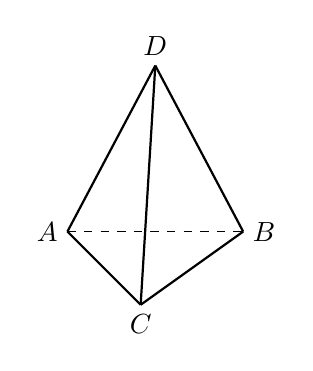
\begin{tikzpicture}[scale=0.62,>=stealth]
\draw[thick] (0,0)--(1.5,-1.5);
\draw[thick] (3.6,0)--(1.5,-1.5);
\draw[thick] (1.8,3.4)--(0,0);
\draw[thick] (1.8,3.4)--(3.6,0);
\draw[thick] (1.8,3.4)--(1.5,-1.5);
\draw[dashed] (0,0)--(3.6,0);
\node[left] at (0,0){$A$};
\node[right] at (3.6,0){$B$};
\node[below] at (1.5,-1.5){$C$};
\node[above] at (1.8,3.4){$D$};
\end{tikzpicture}
\end{center}
Gọi $I$ là trung điểm của đoạn thẳng $BA$.  Với điểm $M$ bất kì, ta có $\overrightarrow{MB}+\overrightarrow{MA}=k\,\overrightarrow{MI}$. Giá trị của $k$ là}
  {$2$.}
  {$1$.}{$3$.}{$4$.}

\cauTN[id=C2-B6-D01-TH-033,muc=TH,loigiai={Do $G$ là tâm hình hộp (trung điểm mỗi đường chéo) nên $\overrightarrow{OM}+\overrightarrow{ON}+\overrightarrow{OP}+\overrightarrow{OQ}+\overrightarrow{OM'}+\overrightarrow{ON'}+\overrightarrow{OP'}+\overrightarrow{OQ'}=8\,\overrightarrow{OG}$, suy ra $k=8$.}]{Cho hình hộp $MNPQ.M'N'P'Q'$. Gọi $G$ là tâm của hình hộp. Với điểm $O$ bất kì, ta có $\overrightarrow{OM}+\overrightarrow{ON}+\overrightarrow{OP}+\overrightarrow{OQ}+\overrightarrow{OM'}+\overrightarrow{ON'}+\overrightarrow{OP'}+\overrightarrow{OQ'}=k\,\overrightarrow{OG}$. Giá trị của $k$ là}
  {$8$.}
  {$7$.}{$9$.}{$16$.}

\cauTN[id=C2-B6-D01-TH-034,muc=TH,loigiai={Do $G$ là trọng tâm tứ diện nên $\overrightarrow{OM}+\overrightarrow{ON}+\overrightarrow{OP}+\overrightarrow{OQ}=4\,\overrightarrow{OG}$, suy ra $k=4$.}]{Cho tứ diện $MNPQ$. Gọi $G$ là trọng tâm của tứ diện $MNPQ$. Với điểm $O$ bất kì, ta có $\overrightarrow{OM}+\overrightarrow{ON}+\overrightarrow{OP}+\overrightarrow{OQ}=k\,\overrightarrow{OG}$. Giá trị của $k$ là}
  {$4$.}
  {$3$.}{$5$.}{$8$.}

\cauTN[id=C2-B6-D01-TH-035,muc=TH,loigiai={Do $I$ là trung điểm nên $\overrightarrow{MB}+\overrightarrow{MA}=2\,\overrightarrow{MI}$, suy ra $k=2$.}]{Cho tứ diện $ABCD$. Gọi $I$ là trung điểm của đoạn thẳng $BA$. Với điểm $M$ bất kì, ta có $\overrightarrow{MB}+\overrightarrow{MA}=k\,\overrightarrow{MI}$. Giá trị của $k$ là}
  {$2$.}
  {$1$.}{$3$.}{$4$.}

\cauTN[id=C2-B6-D01-TH-036,muc=TH,loigiai={Do $I$ là trung điểm nên $\overrightarrow{MA}+\overrightarrow{MS}=2\,\overrightarrow{MI}$, suy ra $k=2$.}]{Cho tứ diện $SABC$ như hình vẽ.
\begin{center}
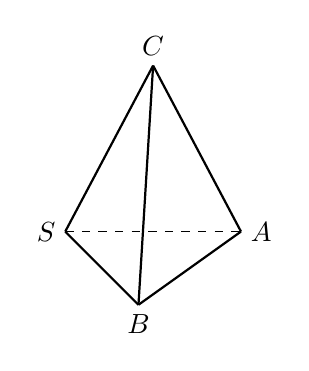
\begin{tikzpicture}[scale=0.62,>=stealth]
\draw[thick] (0,0)--(1.5,-1.5);
\draw[thick] (3.6,0)--(1.5,-1.5);
\draw[thick] (1.8,3.4)--(0,0);
\draw[thick] (1.8,3.4)--(3.6,0);
\draw[thick] (1.8,3.4)--(1.5,-1.5);
\draw[dashed] (0,0)--(3.6,0);
\node[left] at (0,0){$S$};
\node[right] at (3.6,0){$A$};
\node[below] at (1.5,-1.5){$B$};
\node[above] at (1.8,3.4){$C$};
\end{tikzpicture}
\end{center}
Gọi $I$ là trung điểm của đoạn thẳng $AS$.  Với điểm $M$ bất kì, ta có $\overrightarrow{MA}+\overrightarrow{MS}=k\,\overrightarrow{MI}$. Giá trị của $k$ là}
  {$2$.}
  {$1$.}{$3$.}{$4$.}

\cauTN[id=C2-B6-D01-TH-037,muc=TH,loigiai={Ta có $\overrightarrow{Q'P}+\overrightarrow{Q'Q}$ có tọa độ phân tích theo ba cạnh $(1;0;-2)$, trong đó các cạnh đôi một vuông góc nên $|\overrightarrow{Q'P}+\overrightarrow{Q'Q}|^2=5a^2$. Vậy $|\overrightarrow{Q'P}+\overrightarrow{Q'Q}|=a\sqrt{5}$.}]{Cho hình lập phương $MNPQ.M'N'P'Q'$ có cạnh bằng $a$. Độ dài của vectơ $\overrightarrow{Q'P}+\overrightarrow{Q'Q}$ bằng}
  {$a\sqrt{5}$.}
  {$a$.}{$a\sqrt{10}$.}{$a\sqrt{13}$.}

\cauTN[id=C2-B6-D01-TH-038,muc=TH,loigiai={Ta có $\overrightarrow{B'A'}+\overrightarrow{AD}+\overrightarrow{DA'}$ có tọa độ phân tích theo ba cạnh $(-1;0;1)$, trong đó các cạnh đôi một vuông góc nên $|\overrightarrow{B'A'}+\overrightarrow{AD}+\overrightarrow{DA'}|^2=2a^2$. Vậy $|\overrightarrow{B'A'}+\overrightarrow{AD}+\overrightarrow{DA'}|=a\sqrt{2}$.}]{Cho hình lập phương $ABCD.A'B'C'D'$ có cạnh bằng $a$. Độ dài của vectơ $\overrightarrow{B'A'}+\overrightarrow{AD}+\overrightarrow{DA'}$ bằng}
  {$a\sqrt{2}$.}
  {$a\sqrt{3}$.}{$a\sqrt{6}$.}{$a\sqrt{5}$.}

\cauTN[id=C2-B6-D01-TH-039,muc=TH,loigiai={Ta có $2\overrightarrow{EG}+\overrightarrow{DH}+\overrightarrow{HE}$ có tọa độ phân tích theo ba cạnh $(2;1;1)$, trong đó các cạnh đôi một vuông góc nên $|2\overrightarrow{EG}+\overrightarrow{DH}+\overrightarrow{HE}|^2=157$. Vậy $|2\overrightarrow{EG}+\overrightarrow{DH}+\overrightarrow{HE}|=\sqrt{157}$.}]{Cho hình hộp chữ nhật $ABCD.EFGH$ có $AB=6$, $AD=3$, $AE=2$. Độ dài của vectơ $2\overrightarrow{EG}+\overrightarrow{DH}+\overrightarrow{HE}$ bằng}
  {$\sqrt{157}$.}
  {$\sqrt{229}$.}{$2\sqrt{37}$.}{$2\sqrt{10}$.}

\cauTN[id=C2-B6-D01-TH-040,muc=TH,loigiai={Ta có $-\overrightarrow{QP}+2\overrightarrow{M'M}+2\overrightarrow{N'Q'}$ có tọa độ phân tích theo ba cạnh $(-3;2;-2)$, trong đó các cạnh đôi một vuông góc nên $|-\overrightarrow{QP}+2\overrightarrow{M'M}+2\overrightarrow{N'Q'}|^2=109$. Vậy $|-\overrightarrow{QP}+2\overrightarrow{M'M}+2\overrightarrow{N'Q'}|=\sqrt{109}$.}]{Cho hình hộp chữ nhật $MNPQ.M'N'P'Q'$ có $MN=1$, $MQ=3$, $MM'=4$. Độ dài của vectơ $-\overrightarrow{QP}+2\overrightarrow{M'M}+2\overrightarrow{N'Q'}$ bằng}
  {$\sqrt{109}$.}
  {$\sqrt{101}$.}{$\sqrt{61}$.}{$\sqrt{77}$.}

\cauTN[id=C2-B6-D01-TH-041,muc=TH,loigiai={Ta có $\overrightarrow{M'Q'}-\overrightarrow{P'N}$ có tọa độ phân tích theo ba cạnh $(0;2;1)$, trong đó các cạnh đôi một vuông góc nên $|\overrightarrow{M'Q'}-\overrightarrow{P'N}|^2=13$. Vậy $|\overrightarrow{M'Q'}-\overrightarrow{P'N}|=\sqrt{13}$.}]{Cho hình hộp chữ nhật $MNPQ.M'N'P'Q'$ có $MN=6$, $MQ=1$, $MM'=3$. Độ dài của vectơ $\overrightarrow{M'Q'}-\overrightarrow{P'N}$ bằng}
  {$\sqrt{13}$.}
  {$3\sqrt{2}$.}{$3$.}{$3\sqrt{5}$.}

\cauTN[id=C2-B6-D01-TH-042,muc=TH,loigiai={Ta có $2\overrightarrow{BD'}+2\overrightarrow{D'C}+\overrightarrow{BD}$ có tọa độ phân tích theo ba cạnh $(-1;3;0)$, trong đó các cạnh đôi một vuông góc nên $|2\overrightarrow{BD'}+2\overrightarrow{D'C}+\overrightarrow{BD}|^2=37$. Vậy $|2\overrightarrow{BD'}+2\overrightarrow{D'C}+\overrightarrow{BD}|=\sqrt{37}$.}]{Cho hình hộp chữ nhật $ABCD.A'B'C'D'$ có $AB=1$, $AD=2$, $AA'=4$. Độ dài của vectơ $2\overrightarrow{BD'}+2\overrightarrow{D'C}+\overrightarrow{BD}$ bằng}
  {$\sqrt{37}$.}
  {$\sqrt{317}$.}{$2\sqrt{14}$.}{$2\sqrt{17}$.}

\cauTN[id=C2-B6-D01-TH-043,muc=TH,loigiai={Ta có $2\overrightarrow{H'E}-\overrightarrow{EG}+\overrightarrow{FE'}$ có tọa độ phân tích theo ba cạnh $(-2;-3;-1)$, trong đó các cạnh đôi một vuông góc nên $|2\overrightarrow{H'E}-\overrightarrow{EG}+\overrightarrow{FE'}|^2=292$. Vậy $|2\overrightarrow{H'E}-\overrightarrow{EG}+\overrightarrow{FE'}|=2\sqrt{73}$.}]{Cho hình hộp chữ nhật $EFGH.E'F'G'H'$ có $EF=6$, $EH=4$, $EE'=2$. Độ dài của vectơ $2\overrightarrow{H'E}-\overrightarrow{EG}+\overrightarrow{FE'}$ bằng}
  {$2\sqrt{73}$.}
  {$14$.}{$2\sqrt{146}$.}{$6\sqrt{13}$.}

\cauTN[id=C2-B6-D01-TH-044,muc=TH,loigiai={Ta có $-\overrightarrow{NN'}+\overrightarrow{QP}-\overrightarrow{N'P'}$ có tọa độ phân tích theo ba cạnh $(1;-1;-1)$, trong đó các cạnh đôi một vuông góc nên $|-\overrightarrow{NN'}+\overrightarrow{QP}-\overrightarrow{N'P'}|^2=61$. Vậy $|-\overrightarrow{NN'}+\overrightarrow{QP}-\overrightarrow{N'P'}|=\sqrt{61}$.}]{Cho hình hộp chữ nhật $MNPQ.M'N'P'Q'$ có $MN=6$, $MQ=3$, $MM'=4$. Độ dài của vectơ $-\overrightarrow{NN'}+\overrightarrow{QP}-\overrightarrow{N'P'}$ bằng}
  {$\sqrt{61}$.}
  {$\sqrt{109}$.}{$2\sqrt{22}$.}{$13$.}

\cauTN[id=C2-B6-D01-TH-045,muc=TH,loigiai={Ta có $2\overrightarrow{DA}+\overrightarrow{D'C}+2\overrightarrow{DA'}$ có tọa độ phân tích theo ba cạnh $(1;-4;1)$, trong đó các cạnh đôi một vuông góc nên $|2\overrightarrow{DA}+\overrightarrow{D'C}+2\overrightarrow{DA'}|^2=164$. Vậy $|2\overrightarrow{DA}+\overrightarrow{D'C}+2\overrightarrow{DA'}|=2\sqrt{41}$.}]{Cho hình hộp chữ nhật $ABCD.A'B'C'D'$ có $AB=2$, $AD=3$, $AA'=4$. Độ dài của vectơ $2\overrightarrow{DA}+\overrightarrow{D'C}+2\overrightarrow{DA'}$ bằng}
  {$2\sqrt{41}$.}
  {$\sqrt{85}$.}{$2\sqrt{73}$.}{$4\sqrt{10}$.}

\cauTN[id=C2-B6-D01-TH-046,muc=TH,loigiai={Ta có $-\overrightarrow{FH}+\overrightarrow{CG}+2\overrightarrow{CB}$ có tọa độ phân tích theo ba cạnh $(1;-3;1)$, trong đó các cạnh đôi một vuông góc nên $|-\overrightarrow{FH}+\overrightarrow{CG}+2\overrightarrow{CB}|^2=11a^2$. Vậy $|-\overrightarrow{FH}+\overrightarrow{CG}+2\overrightarrow{CB}|=a\sqrt{11}$.}]{Cho hình lập phương $ABCD.EFGH$ có cạnh bằng $a$. Độ dài của vectơ $-\overrightarrow{FH}+\overrightarrow{CG}+2\overrightarrow{CB}$ bằng}
  {$a\sqrt{11}$.}
  {$a\sqrt{3}$.}{$a\sqrt{14}$.}{$a\sqrt{6}$.}

\cauTN[id=C2-B6-D01-TH-047,muc=TH,loigiai={Ta có $-\overrightarrow{FE}+2\overrightarrow{BH}$ có tọa độ phân tích theo ba cạnh $(-1;2;2)$, trong đó các cạnh đôi một vuông góc nên $|-\overrightarrow{FE}+2\overrightarrow{BH}|^2=68$. Vậy $|-\overrightarrow{FE}+2\overrightarrow{BH}|=2\sqrt{17}$.}]{Cho hình hộp chữ nhật $ABCD.EFGH$ có $AB=4$, $AD=2$, $AE=3$. Độ dài của vectơ $-\overrightarrow{FE}+2\overrightarrow{BH}$ bằng}
  {$2\sqrt{17}$.}
  {$2\sqrt{13}$.}{$\sqrt{13}$.}{$14$.}

\cauTN[id=C2-B6-D01-TH-048,muc=TH,loigiai={Ta có $2\overrightarrow{EF}+2\overrightarrow{AD}+\overrightarrow{BG}$ có tọa độ phân tích theo ba cạnh $(2;3;1)$, trong đó các cạnh đôi một vuông góc nên $|2\overrightarrow{EF}+2\overrightarrow{AD}+\overrightarrow{BG}|^2=364$. Vậy $|2\overrightarrow{EF}+2\overrightarrow{AD}+\overrightarrow{BG}|=2\sqrt{91}$.}]{Cho hình hộp chữ nhật $ABCD.EFGH$ có $AB=3$, $AD=6$, $AE=2$. Độ dài của vectơ $2\overrightarrow{EF}+2\overrightarrow{AD}+\overrightarrow{BG}$ bằng}
  {$2\sqrt{91}$.}
  {$2\sqrt{157}$.}{$2\sqrt{19}$.}{$\sqrt{337}$.}

\cauDS[id=C2-B6-D01-TH-049,muc=TH,loigiai={Sử dụng quy tắc cộng, trừ vectơ, tính chất trung điểm và trọng tâm. a) Sai. b) Sai. c) Đúng. d) Sai.}]{Cho hình hộp $ABCD.A'B'C'D'$. Gọi $G$ là trọng tâm của tam giác $D'C'A'$. Gọi $I$ là trung điểm của đoạn thẳng $AA'$. Xét tính đúng sai của các mệnh đề sau:}{%
  \y{$\overrightarrow{GD'}=\overrightarrow{GC'}+\overrightarrow{GA'}$.}{s}
  \y{$\overrightarrow{BC}+\overrightarrow{CC'}=\overrightarrow{BD}$.}{s}
  \y{$\overrightarrow{DC'}-\overrightarrow{D'C'}=\overrightarrow{DD'}$.}{d}
  \y{$\overrightarrow{D'A}-\overrightarrow{C'A}=\overrightarrow{D'B'}$.}{s}}

\cauDS[id=C2-B6-D01-TH-050,muc=TH,loigiai={Sử dụng quy tắc cộng, trừ vectơ, tính chất trung điểm và trọng tâm. a) Đúng. b) Đúng. c) Đúng. d) Sai.}]{Cho hình hộp $ABCD.A'B'C'D'$. Gọi $I$ là trung điểm của đoạn thẳng $BA$. Gọi $G$ là trọng tâm của tam giác $C'BA$. Xét tính đúng sai của các mệnh đề sau:}{%
  \y{$\overrightarrow{BA}=2\overrightarrow{BI}$.}{d}
  \y{$\overrightarrow{D'C'}+\overrightarrow{D'B}+\overrightarrow{D'A}=3\overrightarrow{D'G}$.}{d}
  \y{$\overrightarrow{BI}=\overrightarrow{IA}$.}{d}
  \y{$\overrightarrow{B'C'}+\overrightarrow{B'B}+\overrightarrow{B'A}=2\overrightarrow{B'G}$.}{s}}

\cauDS[id=C2-B6-D01-TH-051,muc=TH,loigiai={Sử dụng quy tắc cộng, trừ vectơ, tính chất trung điểm và trọng tâm. a) Sai. b) Đúng. c) Đúng. d) Sai.}]{Cho tứ diện $MNPQ$ như hình vẽ.
\begin{center}
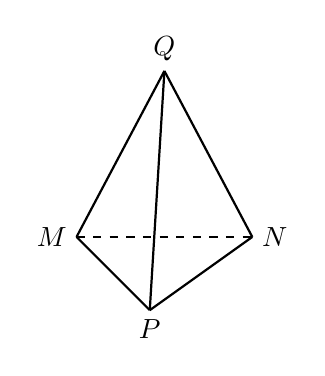
\begin{tikzpicture}[scale=0.62,>=stealth]
\draw[thick] (0,0)--(1.5,-1.5);
\draw[thick] (3.6,0)--(1.5,-1.5);
\draw[thick] (1.8,3.4)--(0,0);
\draw[thick] (1.8,3.4)--(3.6,0);
\draw[thick] (1.8,3.4)--(1.5,-1.5);
\draw[dashed] (0,0)--(3.6,0);
\node[left] at (0,0){$M$};
\node[right] at (3.6,0){$N$};
\node[below] at (1.5,-1.5){$P$};
\node[above] at (1.8,3.4){$Q$};
\end{tikzpicture}
\end{center}
Gọi $I$ là trung điểm của đoạn thẳng $QP$. Gọi $G$ là trọng tâm của tam giác $MPN$.  Xét tính đúng sai của các mệnh đề sau:}{%
  \y{$\overrightarrow{NQ}+\overrightarrow{NP}=\overrightarrow{NI}$.}{s}
  \y{$\overrightarrow{IQ}=-\overrightarrow{IP}$.}{d}
  \y{$\overrightarrow{NQ}+\overrightarrow{NP}=2\overrightarrow{NI}$.}{d}
  \y{$\overrightarrow{GM}+\overrightarrow{GP}=\overrightarrow{GN}$.}{s}}

\cauDS[id=C2-B6-D01-TH-052,muc=TH,loigiai={Sử dụng quy tắc cộng, trừ vectơ, tính chất trung điểm và trọng tâm. a) Đúng. b) Đúng. c) Sai. d) Sai.}]{Cho hình hộp $ABCD.EFGH$. Gọi $I$ là trung điểm của đoạn thẳng $BH$. Gọi $J$ là trọng tâm của tam giác $HGE$. Xét tính đúng sai của các mệnh đề sau:}{%
  \y{$\overrightarrow{IB}=-\overrightarrow{IH}$.}{d}
  \y{$\overrightarrow{DA}+\overrightarrow{DH}+\overrightarrow{DC}=\overrightarrow{DF}$.}{d}
  \y{$\overrightarrow{AB}+\overrightarrow{AH}=\overrightarrow{AI}$.}{s}
  \y{$\overrightarrow{CB}+\overrightarrow{CH}=3\overrightarrow{CI}$.}{s}}

\cauDS[id=C2-B6-D01-TH-053,muc=TH,loigiai={Sử dụng quy tắc cộng, trừ vectơ, tính chất trung điểm và trọng tâm. a) Đúng. b) Đúng. c) Sai. d) Đúng.}]{Cho tứ diện $ABCD$. Gọi $I$ là trung điểm của đoạn thẳng $DB$. Gọi $G$ là trọng tâm của tam giác $DAB$. Xét tính đúng sai của các mệnh đề sau:}{%
  \y{$\overrightarrow{CD}+\overrightarrow{CB}=2\overrightarrow{CI}$.}{d}
  \y{$\overrightarrow{GD}=-\overrightarrow{GA}-\overrightarrow{GB}$.}{d}
  \y{$\overrightarrow{CD}+\overrightarrow{CA}+\overrightarrow{CB}=2\overrightarrow{CG}$.}{s}
  \y{$\overrightarrow{ID}=-\overrightarrow{IB}$.}{d}}

\cauDS[id=C2-B6-D01-TH-054,muc=TH,loigiai={Sử dụng quy tắc cộng, trừ vectơ, tính chất trung điểm và trọng tâm. a) Đúng. b) Sai. c) Sai. d) Đúng.}]{Cho hình hộp $ABCD.A'B'C'D'$. Gọi $I$ là trung điểm của đoạn thẳng $C'C$. Gọi $G$ là trọng tâm của tam giác $A'B'D$. Xét tính đúng sai của các mệnh đề sau:}{%
  \y{$\overrightarrow{A'D'}+\overrightarrow{A'A}+\overrightarrow{A'B'}=\overrightarrow{A'C}$.}{d}
  \y{$\overrightarrow{A'C'}+\overrightarrow{A'C}=3\overrightarrow{A'I}$.}{s}
  \y{$\overrightarrow{BC}+\overrightarrow{BB'}+\overrightarrow{BA}=\overrightarrow{BA}$.}{s}
  \y{$\overrightarrow{C'A'}+\overrightarrow{C'B'}+\overrightarrow{C'D}=3\overrightarrow{C'G}$.}{d}}

\cauDS[id=C2-B6-D01-TH-055,muc=TH,loigiai={Sử dụng quy tắc cộng, trừ vectơ, tính chất trung điểm và trọng tâm. a) Sai. b) Sai. c) Đúng. d) Đúng.}]{Cho hình chóp $S.ABCD$ có đáy $ABCD$ là hình bình hành như hình vẽ.
\begin{center}
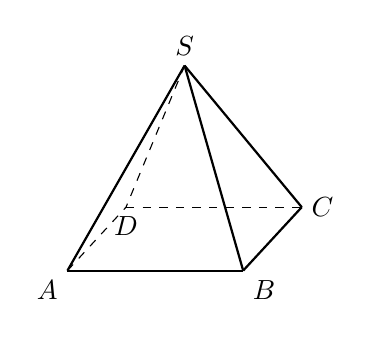
\begin{tikzpicture}[scale=0.62,>=stealth]
\draw[thick] (0,0)--(3.6,0);
\draw[thick] (3.6,0)--(4.8,1.3);
\draw[thick] (2.4,4.2)--(0,0);
\draw[thick] (2.4,4.2)--(3.6,0);
\draw[thick] (2.4,4.2)--(4.8,1.3);
\draw[dashed] (0,0)--(1.2,1.3);
\draw[dashed] (1.2,1.3)--(4.8,1.3);
\draw[dashed] (2.4,4.2)--(1.2,1.3);
\node[below left] at (0,0){$A$};
\node[below right] at (3.6,0){$B$};
\node[right] at (4.8,1.3){$C$};
\node[below] at (1.2,1.3){$D$};
\node[above] at (2.4,4.2){$S$};
\end{tikzpicture}
\end{center}
Gọi $O$ là giao điểm của hai đường chéo $AC$ và $BD$. Gọi $I$ là trung điểm của đoạn thẳng $DA$.  Xét tính đúng sai của các mệnh đề sau:}{%
  \y{$\overrightarrow{BD}+\overrightarrow{BA}=\overrightarrow{BI}$.}{s}
  \y{$\overrightarrow{SD}+\overrightarrow{DA}=\overrightarrow{SC}$.}{s}
  \y{$\overrightarrow{AB}-\overrightarrow{CB}=\overrightarrow{AC}$.}{d}
  \y{$\overrightarrow{DA}=2\overrightarrow{IA}$.}{d}}

\cauDS[id=C2-B6-D01-TH-056,muc=TH,loigiai={Sử dụng quy tắc cộng, trừ vectơ, tính chất trung điểm và trọng tâm. a) Sai. b) Đúng. c) Đúng. d) Sai.}]{Cho hình hộp $ABCD.A'B'C'D'$. Gọi $G$ là trọng tâm của tam giác $DA'B$. Gọi $I$ là trung điểm của đoạn thẳng $B'D'$. Xét tính đúng sai của các mệnh đề sau:}{%
  \y{$\overrightarrow{GD}+\overrightarrow{GA'}=\overrightarrow{GB}$.}{s}
  \y{$\overrightarrow{GD}+\overrightarrow{GA'}=\overrightarrow{BG}$.}{d}
  \y{$\overrightarrow{DB}-\overrightarrow{C'B}=\overrightarrow{DC'}$.}{d}
  \y{$\overrightarrow{CD'}-\overrightarrow{C'D'}=\overrightarrow{CD}$.}{s}}

\cauDS[id=C2-B6-D01-TH-057,muc=TH,loigiai={Sử dụng quy tắc cộng, trừ vectơ, tính chất trung điểm và trọng tâm. a) Sai. b) Sai. c) Đúng. d) Đúng.}]{Cho hình hộp $EFGH.E'F'G'H'$ như hình vẽ.
\begin{center}
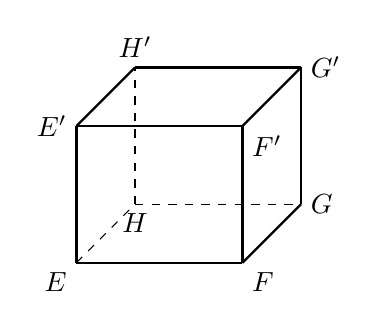
\begin{tikzpicture}[scale=0.62,>=stealth]
\draw[thick] (0,0)--(3.4,0);
\draw[thick] (3.4,0)--(4.6,1.2);
\draw[thick] (4.6,1.2)--(4.6,4.0);
\draw[thick] (0,2.8)--(3.4,2.8);
\draw[thick] (3.4,2.8)--(4.6,4.0);
\draw[thick] (4.6,4.0)--(1.2,4.0);
\draw[thick] (1.2,4.0)--(0,2.8);
\draw[thick] (0,0)--(0,2.8);
\draw[thick] (3.4,0)--(3.4,2.8);
\draw[dashed] (0,0)--(1.2,1.2);
\draw[dashed] (1.2,1.2)--(4.6,1.2);
\draw[dashed] (1.2,1.2)--(1.2,4.0);
\node[below left] at (0,0){$E$};
\node[below right] at (3.4,0){$F$};
\node[right] at (4.6,1.2){$G$};
\node[below] at (1.2,1.2){$H$};
\node[left] at (0,2.8){$E'$};
\node[below right] at (3.4,2.8){$F'$};
\node[right] at (4.6,4.0){$G'$};
\node[above] at (1.2,4.0){$H'$};
\end{tikzpicture}
\end{center}
Gọi $J$ là trọng tâm của tam giác $H'HG$. Gọi $I$ là trung điểm của đoạn thẳng $F'E'$.  Xét tính đúng sai của các mệnh đề sau:}{%
  \y{$\overrightarrow{G'F'}+\overrightarrow{G'H'}+\overrightarrow{G'G}=\overrightarrow{G'E'}$.}{s}
  \y{$\overrightarrow{HG}+\overrightarrow{HE}+\overrightarrow{HH'}=\overrightarrow{HF}$.}{s}
  \y{$\overrightarrow{F'F}+\overrightarrow{F'E'}+\overrightarrow{F'G'}=\overrightarrow{F'H}$.}{d}
  \y{$\overrightarrow{H'E'}+\overrightarrow{H'G'}+\overrightarrow{H'H}=\overrightarrow{H'F}$.}{d}}

\cauDS[id=C2-B6-D01-TH-058,muc=TH,loigiai={Sử dụng quy tắc cộng, trừ vectơ, tính chất trung điểm và trọng tâm. a) Đúng. b) Đúng. c) Đúng. d) Sai.}]{Cho tứ diện $SABC$. Gọi $G$ là trọng tâm của tam giác $ABS$. Gọi $H$ là trọng tâm của tứ diện $SABC$. Xét tính đúng sai của các mệnh đề sau:}{%
  \y{$\overrightarrow{AC}+\overrightarrow{CS}=\overrightarrow{AS}$.}{d}
  \y{$\overrightarrow{HS}+\overrightarrow{HA}+\overrightarrow{HB}+\overrightarrow{HC}=\overrightarrow{0}$.}{d}
  \y{$\overrightarrow{GA}=-\overrightarrow{GB}-\overrightarrow{GS}$.}{d}
  \y{$\overrightarrow{GA}=\overrightarrow{GB}+\overrightarrow{GS}$.}{s}}

\cauDS[id=C2-B6-D01-TH-059,muc=TH,loigiai={Sử dụng quy tắc cộng, trừ vectơ, tính chất trung điểm và trọng tâm. a) Sai. b) Sai. c) Đúng. d) Sai.}]{Cho hình hộp $ABCD.A'B'C'D'$. Gọi $I$ là trung điểm của đoạn thẳng $AD$. Gọi $G$ là trọng tâm của tam giác $CD'A'$. Xét tính đúng sai của các mệnh đề sau:}{%
  \y{$\overrightarrow{D'A}+\overrightarrow{D'D}=\overrightarrow{D'I}$.}{s}
  \y{$\overrightarrow{B'C'}+\overrightarrow{B'B}=\overrightarrow{B'A}$.}{s}
  \y{$\overrightarrow{GC}+\overrightarrow{GD'}=\overrightarrow{A'G}$.}{d}
  \y{$\overrightarrow{C'A}+\overrightarrow{C'D}=\overrightarrow{C'I}$.}{s}}

\cauDS[id=C2-B6-D01-TH-060,muc=TH,loigiai={Sử dụng quy tắc cộng, trừ vectơ, tính chất trung điểm và trọng tâm. a) Sai. b) Đúng. c) Sai. d) Sai.}]{Cho hình chóp $S.MNPQ$ có đáy $MNPQ$ là hình bình hành. Gọi $O$ là giao điểm của hai đường chéo $MP$ và $NQ$. Gọi $I$ là trung điểm của đoạn thẳng $PM$. Xét tính đúng sai của các mệnh đề sau:}{%
  \y{$\overrightarrow{MP}-\overrightarrow{QP}=\overrightarrow{MS}$.}{s}
  \y{$\overrightarrow{PS}-\overrightarrow{NS}=\overrightarrow{PN}$.}{d}
  \y{$\overrightarrow{SM}+\overrightarrow{SP}=\overrightarrow{SO}$.}{s}
  \y{$\overrightarrow{NP}-\overrightarrow{SP}=\overrightarrow{NM}$.}{s}}

\cauDS[id=C2-B6-D01-TH-061,muc=TH,loigiai={Sử dụng quy tắc cộng, trừ vectơ, tính chất trung điểm và trọng tâm. a) Sai. b) Đúng. c) Đúng. d) Đúng.}]{Cho tứ diện $SABC$. Gọi $G$ là trọng tâm của tam giác $BAC$. Gọi $H$ là trọng tâm của tứ diện $SABC$. Xét tính đúng sai của các mệnh đề sau:}{%
  \y{$\overrightarrow{BS}+\overrightarrow{BA}+\overrightarrow{BC}=3\overrightarrow{BH}$.}{s}
  \y{$\overrightarrow{AS}+\overrightarrow{AB}+\overrightarrow{AC}=4\overrightarrow{AH}$.}{d}
  \y{$\overrightarrow{GB}=-\overrightarrow{GA}-\overrightarrow{GC}$.}{d}
  \y{$\overrightarrow{GB}+\overrightarrow{GA}=\overrightarrow{CG}$.}{d}}

\cauDS[id=C2-B6-D01-TH-062,muc=TH,loigiai={Sử dụng quy tắc cộng, trừ vectơ, tính chất trung điểm và trọng tâm. a) Sai. b) Sai. c) Đúng. d) Sai.}]{Cho hình hộp $EFGH.E'F'G'H'$. Gọi $I$ là trung điểm của đoạn thẳng $HE$. Gọi $J$ là trọng tâm của tam giác $G'FE'$. Xét tính đúng sai của các mệnh đề sau:}{%
  \y{$\overrightarrow{FF'}+\overrightarrow{FG}=\overrightarrow{FH'}$.}{s}
  \y{$\overrightarrow{H'H}+\overrightarrow{H'G'}=\overrightarrow{H'E}$.}{s}
  \y{$\overrightarrow{HE}=2\overrightarrow{HI}$.}{d}
  \y{$\overrightarrow{FE'}+\overrightarrow{FG}=\overrightarrow{FG}$.}{s}}

\cauDS[id=C2-B6-D01-TH-063,muc=TH,loigiai={Sử dụng quy tắc cộng, trừ vectơ, tính chất trung điểm và trọng tâm. a) Sai. b) Đúng. c) Sai. d) Sai.}]{Cho hình hộp $EFGH.E'F'G'H'$. Gọi $I$ là trung điểm của đoạn thẳng $H'F'$. Gọi $J$ là trọng tâm của tam giác $EHF$. Xét tính đúng sai của các mệnh đề sau:}{%
  \y{$\overrightarrow{JE}=\overrightarrow{JH}+\overrightarrow{JF}$.}{s}
  \y{$\overrightarrow{G'F'}+\overrightarrow{G'H'}+\overrightarrow{G'G}=\overrightarrow{G'E}$.}{d}
  \y{$\overrightarrow{E'E}+\overrightarrow{E'H'}+\overrightarrow{E'F'}=\overrightarrow{E'E}$.}{s}
  \y{$\overrightarrow{JE}+\overrightarrow{JH}=\overrightarrow{JF}$.}{s}}

\cauDS[id=C2-B6-D01-TH-064,muc=TH,loigiai={Sử dụng quy tắc cộng, trừ vectơ, tính chất trung điểm và trọng tâm. a) Sai. b) Đúng. c) Đúng. d) Sai.}]{Cho tứ diện $ABCD$. Gọi $G$ là trọng tâm của tam giác $CBA$. Gọi $H$ là trọng tâm của tứ diện $ABCD$. Xét tính đúng sai của các mệnh đề sau:}{%
  \y{$\overrightarrow{CG}=\dfrac{1}{2}\overrightarrow{CB}+\dfrac{1}{2}\overrightarrow{CA}$.}{s}
  \y{$\overrightarrow{DC}+\overrightarrow{DB}+\overrightarrow{DA}=3\overrightarrow{DG}$.}{d}
  \y{$\overrightarrow{CG}=\dfrac{1}{3}\overrightarrow{CB}+\dfrac{1}{3}\overrightarrow{CA}$.}{d}
  \y{$\overrightarrow{DC}+\overrightarrow{DB}+\overrightarrow{DA}=2\overrightarrow{DG}$.}{s}}

\cauTLN[id=C2-B6-D01-TH-065,muc=TH,loigiai={Ba cạnh xuất phát từ một đỉnh đôi một vuông góc, $\overrightarrow{C'A'}+2\overrightarrow{A'B}=1;-1;-2$ nên $|\overrightarrow{C'A'}+2\overrightarrow{A'B}|^2=41$.}]{Cho hình hộp chữ nhật $ABCD.A'B'C'D'$ có $AB=4$, $AD=3$, $AA'=2$. Tính $\left|\overrightarrow{C'A'}+2\overrightarrow{A'B}\right|^2$.}{41}

\cauTLN[id=C2-B6-D01-TH-066,muc=TH,loigiai={Ba cạnh xuất phát từ một đỉnh đôi một vuông góc, $2\overrightarrow{A'D}+\overrightarrow{D'D}+2\overrightarrow{CB}=0;0;-3$ nên $|2\overrightarrow{A'D}+\overrightarrow{D'D}+2\overrightarrow{CB}|^2=9$.}]{Cho hình hộp chữ nhật $ABCD.A'B'C'D'$ có $AB=4$, $AD=4$, $AA'=1$. Tính $\left|2\overrightarrow{A'D}+\overrightarrow{D'D}+2\overrightarrow{CB}\right|^2$.}{9}

\cauTLN[id=C2-B6-D01-TH-067,muc=TH,loigiai={Ta có $-\overrightarrow{EH}+\overrightarrow{FE'}=-\vec{a}-\vec{b}+\vec{c}$ nên $x=-1$, $y=-1$, $z=1$. Vậy $T=-1$.}]{Cho hình hộp $EFGH.E'F'G'H'$ như hình vẽ.
\begin{center}
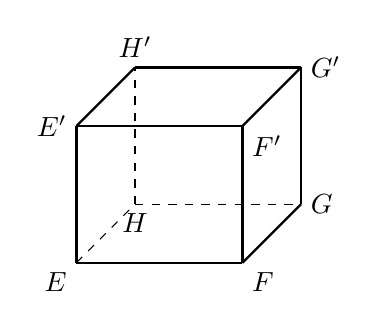
\begin{tikzpicture}[scale=0.62,>=stealth]
\draw[thick] (0,0)--(3.4,0);
\draw[thick] (3.4,0)--(4.6,1.2);
\draw[thick] (4.6,1.2)--(4.6,4.0);
\draw[thick] (0,2.8)--(3.4,2.8);
\draw[thick] (3.4,2.8)--(4.6,4.0);
\draw[thick] (4.6,4.0)--(1.2,4.0);
\draw[thick] (1.2,4.0)--(0,2.8);
\draw[thick] (0,0)--(0,2.8);
\draw[thick] (3.4,0)--(3.4,2.8);
\draw[dashed] (0,0)--(1.2,1.2);
\draw[dashed] (1.2,1.2)--(4.6,1.2);
\draw[dashed] (1.2,1.2)--(1.2,4.0);
\node[below left] at (0,0){$E$};
\node[below right] at (3.4,0){$F$};
\node[right] at (4.6,1.2){$G$};
\node[below] at (1.2,1.2){$H$};
\node[left] at (0,2.8){$E'$};
\node[below right] at (3.4,2.8){$F'$};
\node[right] at (4.6,4.0){$G'$};
\node[above] at (1.2,4.0){$H'$};
\end{tikzpicture}
\end{center}
 Đặt $\vec{a}=\overrightarrow{EF}$, $\vec{b}=\overrightarrow{EH}$, $\vec{c}=\overrightarrow{EE'}$. Biết $-\overrightarrow{EH}+\overrightarrow{FE'}=x\vec{a}+y\vec{b}+z\vec{c}$. Tính $T=3x-y+z$.}{-1}

\cauTLN[id=C2-B6-D01-TH-068,muc=TH,loigiai={Ta có $\overrightarrow{CB}+2\overrightarrow{SC}=\vec{b}+\vec{c}$ nên $x=0$, $y=1$, $z=1$. Vậy $T=3$.}]{Cho tứ diện $SABC$. Đặt $\vec{a}=\overrightarrow{SA}$, $\vec{b}=\overrightarrow{SB}$, $\vec{c}=\overrightarrow{SC}$. Biết $\overrightarrow{CB}+2\overrightarrow{SC}=x\vec{a}+y\vec{b}+z\vec{c}$. Tính $T=3x+y+2z$.}{3}

\cauTLN[id=C2-B6-D01-TH-069,muc=TH,loigiai={Ta có $\overrightarrow{N'Q}+\overrightarrow{NQ'}=-2\vec{a}+2\vec{b}$ nên $x=-2$, $y=2$, $z=0$. Vậy $T=2$.}]{Cho hình hộp $MNPQ.M'N'P'Q'$ như hình vẽ.
\begin{center}
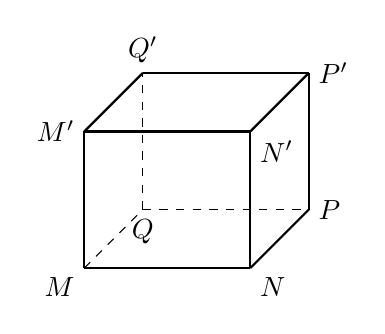
\begin{tikzpicture}[scale=0.62,>=stealth]
\draw[thick] (0,0)--(3.4,0);
\draw[thick] (3.4,0)--(4.6,1.2);
\draw[thick] (4.6,1.2)--(4.6,4.0);
\draw[thick] (0,2.8)--(3.4,2.8);
\draw[thick] (3.4,2.8)--(4.6,4.0);
\draw[thick] (4.6,4.0)--(1.2,4.0);
\draw[thick] (1.2,4.0)--(0,2.8);
\draw[thick] (0,0)--(0,2.8);
\draw[thick] (3.4,0)--(3.4,2.8);
\draw[dashed] (0,0)--(1.2,1.2);
\draw[dashed] (1.2,1.2)--(4.6,1.2);
\draw[dashed] (1.2,1.2)--(1.2,4.0);
\node[below left] at (0,0){$M$};
\node[below right] at (3.4,0){$N$};
\node[right] at (4.6,1.2){$P$};
\node[below] at (1.2,1.2){$Q$};
\node[left] at (0,2.8){$M'$};
\node[below right] at (3.4,2.8){$N'$};
\node[right] at (4.6,4.0){$P'$};
\node[above] at (1.2,4.0){$Q'$};
\end{tikzpicture}
\end{center}
 Đặt $\vec{a}=\overrightarrow{MN}$, $\vec{b}=\overrightarrow{MQ}$, $\vec{c}=\overrightarrow{MM'}$. Biết $\overrightarrow{N'Q}+\overrightarrow{NQ'}=x\vec{a}+y\vec{b}+z\vec{c}$. Tính $T=2x+3y+z$.}{2}

\cauTLN[id=C2-B6-D01-TH-070,muc=TH,loigiai={Ba cạnh xuất phát từ một đỉnh đôi một vuông góc, $-\overrightarrow{BE}-\overrightarrow{FC}+\overrightarrow{GD}=0;-1;-1$ nên $|-\overrightarrow{BE}-\overrightarrow{FC}+\overrightarrow{GD}|^2=17$.}]{Cho hình hộp chữ nhật $ABCD.EFGH$ có $AB=1$, $AD=4$, $AE=1$. Tính $\left|-\overrightarrow{BE}-\overrightarrow{FC}+\overrightarrow{GD}\right|^2$.}{17}

\cauTLN[id=C2-B6-D01-TH-071,muc=TH,loigiai={Ta có $-\overrightarrow{PM}=\vec{a}+\vec{b}$ nên $x=1$, $y=1$, $z=0$. Vậy $T=0$.}]{Cho hình chóp $S.MNPQ$ có đáy $MNPQ$ là hình bình hành. Đặt $\vec{a}=\overrightarrow{MN}$, $\vec{b}=\overrightarrow{MQ}$, $\vec{c}=\overrightarrow{MS}$. Biết $-\overrightarrow{PM}=x\vec{a}+y\vec{b}+z\vec{c}$. Tính $T=2x-2y-z$.}{0}

\cauTLN[id=C2-B6-D01-TH-072,muc=TH,loigiai={Ta có $\overrightarrow{QN}+2\overrightarrow{PQ}=-\vec{a}-\vec{b}$ nên $x=-1$, $y=-1$, $z=0$. Vậy $T=-4$.}]{Cho hình chóp $S.MNPQ$ có đáy $MNPQ$ là hình bình hành như hình vẽ.
\begin{center}
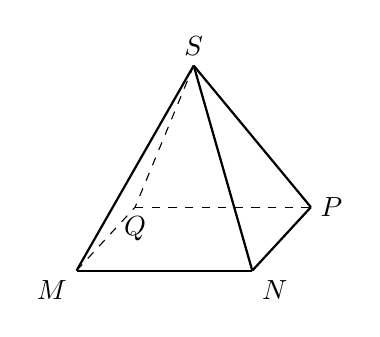
\begin{tikzpicture}[scale=0.62,>=stealth]
\draw[thick] (0,0)--(3.6,0);
\draw[thick] (3.6,0)--(4.8,1.3);
\draw[thick] (2.4,4.2)--(0,0);
\draw[thick] (2.4,4.2)--(3.6,0);
\draw[thick] (2.4,4.2)--(4.8,1.3);
\draw[dashed] (0,0)--(1.2,1.3);
\draw[dashed] (1.2,1.3)--(4.8,1.3);
\draw[dashed] (2.4,4.2)--(1.2,1.3);
\node[below left] at (0,0){$M$};
\node[below right] at (3.6,0){$N$};
\node[right] at (4.8,1.3){$P$};
\node[below] at (1.2,1.3){$Q$};
\node[above] at (2.4,4.2){$S$};
\end{tikzpicture}
\end{center}
 Đặt $\vec{a}=\overrightarrow{MN}$, $\vec{b}=\overrightarrow{MQ}$, $\vec{c}=\overrightarrow{MS}$. Biết $\overrightarrow{QN}+2\overrightarrow{PQ}=x\vec{a}+y\vec{b}+z\vec{c}$. Tính $T=2x+2y+z$.}{-4}

\cauTLN[id=C2-B6-D01-TH-073,muc=TH,loigiai={Ta có $2\overrightarrow{NP'}+2\overrightarrow{M'N}=2\vec{a}+2\vec{b}$ nên $x=2$, $y=2$, $z=0$. Vậy $T=-6$.}]{Cho hình hộp $MNPQ.M'N'P'Q'$. Đặt $\vec{a}=\overrightarrow{MN}$, $\vec{b}=\overrightarrow{MQ}$, $\vec{c}=\overrightarrow{MM'}$. Biết $2\overrightarrow{NP'}+2\overrightarrow{M'N}=x\vec{a}+y\vec{b}+z\vec{c}$. Tính $T=-2x-y+2z$.}{-6}

\cauTLN[id=C2-B6-D01-TH-074,muc=TH,loigiai={Ba cạnh xuất phát từ một đỉnh đôi một vuông góc, $\overrightarrow{EG'}+\overrightarrow{FG'}=1;2;2$ nên $|\overrightarrow{EG'}+\overrightarrow{FG'}|^2=41$.}]{Cho hình hộp chữ nhật $EFGH.E'F'G'H'$ có $EF=1$, $EH=1$, $EE'=3$. Tính $\left|\overrightarrow{EG'}+\overrightarrow{FG'}\right|^2$.}{41}

\cauTLN[id=C2-B6-D01-TH-075,muc=TH,loigiai={Ba cạnh xuất phát từ một đỉnh đôi một vuông góc, $\overrightarrow{F'F}+\overrightarrow{H'G'}+2\overrightarrow{H'H}=1;0;-3$ nên $|\overrightarrow{F'F}+\overrightarrow{H'G'}+2\overrightarrow{H'H}|^2=13$.}]{Cho hình hộp chữ nhật $EFGH.E'F'G'H'$ có $EF=2$, $EH=4$, $EE'=1$. Tính $\left|\overrightarrow{F'F}+\overrightarrow{H'G'}+2\overrightarrow{H'H}\right|^2$.}{13}

\cauTLN[id=C2-B6-D01-TH-076,muc=TH,loigiai={Ta có $\overrightarrow{OC}=\vec{a}+\vec{b}-\vec{c}$ nên $x=1$, $y=1$, $z=-1$. Vậy $T=-1$.}]{Cho hình chóp $O.ABCD$ có đáy $ABCD$ là hình bình hành. Đặt $\vec{a}=\overrightarrow{AB}$, $\vec{b}=\overrightarrow{AD}$, $\vec{c}=\overrightarrow{AO}$. Biết $\overrightarrow{OC}=x\vec{a}+y\vec{b}+z\vec{c}$. Tính $T=x+y+3z$.}{-1}

\cauTLN[id=C2-B6-D01-TH-077,muc=TH,loigiai={Ta có $\overrightarrow{PQ}=-\vec{b}+\vec{c}$ nên $x=0$, $y=-1$, $z=1$. Vậy $T=-4$.}]{Cho tứ diện $MNPQ$ như hình vẽ.
\begin{center}
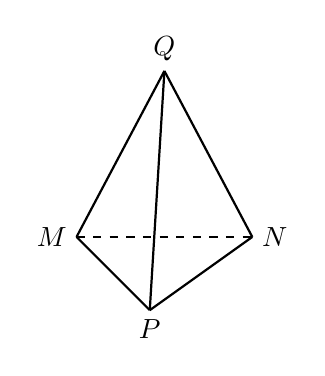
\begin{tikzpicture}[scale=0.62,>=stealth]
\draw[thick] (0,0)--(1.5,-1.5);
\draw[thick] (3.6,0)--(1.5,-1.5);
\draw[thick] (1.8,3.4)--(0,0);
\draw[thick] (1.8,3.4)--(3.6,0);
\draw[thick] (1.8,3.4)--(1.5,-1.5);
\draw[dashed] (0,0)--(3.6,0);
\node[left] at (0,0){$M$};
\node[right] at (3.6,0){$N$};
\node[below] at (1.5,-1.5){$P$};
\node[above] at (1.8,3.4){$Q$};
\end{tikzpicture}
\end{center}
 Đặt $\vec{a}=\overrightarrow{MN}$, $\vec{b}=\overrightarrow{MP}$, $\vec{c}=\overrightarrow{MQ}$. Biết $\overrightarrow{PQ}=x\vec{a}+y\vec{b}+z\vec{c}$. Tính $T=3x+3y-z$.}{-4}

\cauTLN[id=C2-B6-D01-TH-078,muc=TH,loigiai={Ta có $\overrightarrow{CB}+\overrightarrow{CA}=\vec{a}-2\vec{b}$ nên $x=1$, $y=-2$, $z=0$. Vậy $T=-5$.}]{Cho tứ diện $ABCD$ như hình vẽ.
\begin{center}
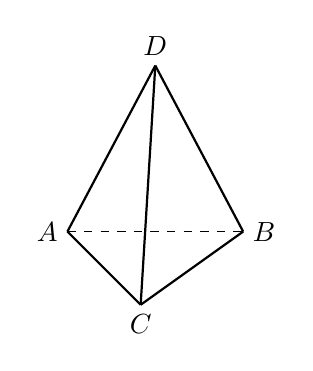
\begin{tikzpicture}[scale=0.62,>=stealth]
\draw[thick] (0,0)--(1.5,-1.5);
\draw[thick] (3.6,0)--(1.5,-1.5);
\draw[thick] (1.8,3.4)--(0,0);
\draw[thick] (1.8,3.4)--(3.6,0);
\draw[thick] (1.8,3.4)--(1.5,-1.5);
\draw[dashed] (0,0)--(3.6,0);
\node[left] at (0,0){$A$};
\node[right] at (3.6,0){$B$};
\node[below] at (1.5,-1.5){$C$};
\node[above] at (1.8,3.4){$D$};
\end{tikzpicture}
\end{center}
 Đặt $\vec{a}=\overrightarrow{AB}$, $\vec{b}=\overrightarrow{AC}$, $\vec{c}=\overrightarrow{AD}$. Biết $\overrightarrow{CB}+\overrightarrow{CA}=x\vec{a}+y\vec{b}+z\vec{c}$. Tính $T=x+3y-2z$.}{-5}

\cauTLN[id=C2-B6-D01-TH-079,muc=TH,loigiai={Ta có $-\overrightarrow{N'P}=-\vec{b}+\vec{c}$ nên $x=0$, $y=-1$, $z=1$. Vậy $T=1$.}]{Cho hình hộp $MNPQ.M'N'P'Q'$. Đặt $\vec{a}=\overrightarrow{MN}$, $\vec{b}=\overrightarrow{MQ}$, $\vec{c}=\overrightarrow{MM'}$. Biết $-\overrightarrow{N'P}=x\vec{a}+y\vec{b}+z\vec{c}$. Tính $T=3x+y+2z$.}{1}

\cauTLN[id=C2-B6-D01-TH-080,muc=TH,loigiai={Ba cạnh xuất phát từ một đỉnh đôi một vuông góc, $-\overrightarrow{B'B}-\overrightarrow{B'D}=1;-1;2$ nên $|-\overrightarrow{B'B}-\overrightarrow{B'D}|^2=61$.}]{Cho hình hộp chữ nhật $ABCD.A'B'C'D'$ có $AB=4$, $AD=3$, $AA'=3$. Tính $\left|-\overrightarrow{B'B}-\overrightarrow{B'D}\right|^2$.}{61}

\cauTN[id=C2-B6-D01-VD-001,muc=VD,loigiai={Do $G$ là trọng tâm tam giác nên $\overrightarrow{QG}=\dfrac{1}{3}(\overrightarrow{QQ'}+\overrightarrow{QM}+\overrightarrow{QM'})$. Phân tích: $\overrightarrow{QQ'}=\vec{c}$, $\overrightarrow{QM}=-\vec{b}$, $\overrightarrow{QM'}=-\vec{b}+\vec{c}$. Cộng lại ta được $\overrightarrow{QG}=-\dfrac{2}{3}\vec{b}+\dfrac{2}{3}\vec{c}$.}]{Cho hình hộp $MNPQ.M'N'P'Q'$. Gọi $G$ là trọng tâm của tam giác $Q'MM'$. Đặt $\vec{a}=\overrightarrow{MN}$, $\vec{b}=\overrightarrow{MQ}$, $\vec{c}=\overrightarrow{MM'}$. Biết $\overrightarrow{QG}=x\vec{a}+y\vec{b}+z\vec{c}$. Bộ số $(x;y;z)$ là}
  {$(0;-\dfrac{2}{3};\dfrac{2}{3})$.}
  {$(\dfrac{2}{3};-\dfrac{2}{3};0)$.}{$(0;\dfrac{2}{3};\dfrac{2}{3})$.}{$(-\dfrac{2}{3};0;\dfrac{2}{3})$.}

\cauTN[id=C2-B6-D01-VD-002,muc=VD,loigiai={Do $J$ là trọng tâm tam giác nên $\overrightarrow{E'J}=\dfrac{1}{3}(\overrightarrow{E'F'}+\overrightarrow{E'H}+\overrightarrow{E'G})$. Phân tích: $\overrightarrow{E'F'}=\vec{a}$, $\overrightarrow{E'H}=\vec{b}-\vec{c}$, $\overrightarrow{E'G}=\vec{a}+\vec{b}-\vec{c}$. Cộng lại ta được $\overrightarrow{E'J}=\dfrac{2}{3}\vec{a}+\dfrac{2}{3}\vec{b}-\dfrac{2}{3}\vec{c}$.}]{Cho hình hộp $EFGH.E'F'G'H'$. Gọi $J$ là trọng tâm của tam giác $F'HG$. Đặt $\vec{a}=\overrightarrow{EF}$, $\vec{b}=\overrightarrow{EH}$, $\vec{c}=\overrightarrow{EE'}$. Biết $\overrightarrow{E'J}=x\vec{a}+y\vec{b}+z\vec{c}$. Bộ số $(x;y;z)$ là}
  {$(\dfrac{2}{3};\dfrac{2}{3};-\dfrac{2}{3})$.}
  {$(\dfrac{2}{3};-\dfrac{2}{3};-\dfrac{2}{3})$.}{$(\dfrac{2}{3};\dfrac{2}{3};0)$.}{$(\dfrac{2}{3};-\dfrac{2}{3};\dfrac{2}{3})$.}

\cauTN[id=C2-B6-D01-VD-003,muc=VD,loigiai={Do $J$ là trọng tâm tam giác nên $\overrightarrow{DJ}=\dfrac{1}{3}(\overrightarrow{DC}+\overrightarrow{DF}+\overrightarrow{DB})$. Phân tích: $\overrightarrow{DC}=\vec{a}$, $\overrightarrow{DF}=\vec{a}-\vec{b}+\vec{c}$, $\overrightarrow{DB}=\vec{a}-\vec{b}$. Cộng lại ta được $\overrightarrow{DJ}=\vec{a}-\dfrac{2}{3}\vec{b}+\dfrac{1}{3}\vec{c}$.}]{Cho hình hộp $ABCD.EFGH$. Gọi $J$ là trọng tâm của tam giác $CFB$. Đặt $\vec{a}=\overrightarrow{AB}$, $\vec{b}=\overrightarrow{AD}$, $\vec{c}=\overrightarrow{AE}$. Biết $\overrightarrow{DJ}=x\vec{a}+y\vec{b}+z\vec{c}$. Bộ số $(x;y;z)$ là}
  {$(1;-\dfrac{2}{3};\dfrac{1}{3})$.}
  {$(\dfrac{1}{3};-\dfrac{2}{3};1)$.}{$(-\dfrac{2}{3};1;\dfrac{1}{3})$.}{$(1;-\dfrac{2}{3};-\dfrac{2}{3})$.}

\cauTN[id=C2-B6-D01-VD-004,muc=VD,loigiai={Do $G$ là trọng tâm tam giác nên $\overrightarrow{SG}=\dfrac{1}{3}(\overrightarrow{SN}+\overrightarrow{SQ}+\overrightarrow{SP})$. Phân tích: $\overrightarrow{SN}=\vec{a}-\vec{c}$, $\overrightarrow{SQ}=\vec{b}-\vec{c}$, $\overrightarrow{SP}=\vec{a}+\vec{b}-\vec{c}$. Cộng lại ta được $\overrightarrow{SG}=\dfrac{2}{3}\vec{a}+\dfrac{2}{3}\vec{b}-\vec{c}$.}]{Cho hình chóp $S.MNPQ$ có đáy $MNPQ$ là hình bình hành. Gọi $G$ là trọng tâm của tam giác $NQP$. Đặt $\vec{a}=\overrightarrow{MN}$, $\vec{b}=\overrightarrow{MQ}$, $\vec{c}=\overrightarrow{MS}$. Biết $\overrightarrow{SG}=x\vec{a}+y\vec{b}+z\vec{c}$. Bộ số $(x;y;z)$ là}
  {$(\dfrac{2}{3};\dfrac{2}{3};-1)$.}
  {$(\dfrac{2}{3};\dfrac{2}{3};-3)$.}{$(\dfrac{2}{3};-1;\dfrac{2}{3})$.}{$(\dfrac{8}{3};\dfrac{2}{3};-1)$.}

\cauTN[id=C2-B6-D01-VD-005,muc=VD,loigiai={Do $I$ là trung điểm nên $\overrightarrow{P'I}=\dfrac{1}{2}(\overrightarrow{P'Q}+\overrightarrow{P'M'})$. Phân tích: $\overrightarrow{P'Q}=-\vec{a}-\vec{c}$, $\overrightarrow{P'M'}=-\vec{a}-\vec{b}$. Cộng lại ta được $\overrightarrow{P'I}=-\vec{a}-\dfrac{1}{2}\vec{b}-\dfrac{1}{2}\vec{c}$.}]{Cho hình hộp $MNPQ.M'N'P'Q'$ như hình vẽ.
\begin{center}
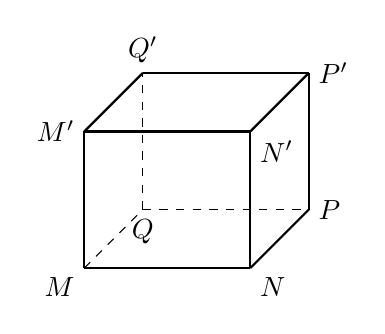
\begin{tikzpicture}[scale=0.62,>=stealth]
\draw[thick] (0,0)--(3.4,0);
\draw[thick] (3.4,0)--(4.6,1.2);
\draw[thick] (4.6,1.2)--(4.6,4.0);
\draw[thick] (0,2.8)--(3.4,2.8);
\draw[thick] (3.4,2.8)--(4.6,4.0);
\draw[thick] (4.6,4.0)--(1.2,4.0);
\draw[thick] (1.2,4.0)--(0,2.8);
\draw[thick] (0,0)--(0,2.8);
\draw[thick] (3.4,0)--(3.4,2.8);
\draw[dashed] (0,0)--(1.2,1.2);
\draw[dashed] (1.2,1.2)--(4.6,1.2);
\draw[dashed] (1.2,1.2)--(1.2,4.0);
\node[below left] at (0,0){$M$};
\node[below right] at (3.4,0){$N$};
\node[right] at (4.6,1.2){$P$};
\node[below] at (1.2,1.2){$Q$};
\node[left] at (0,2.8){$M'$};
\node[below right] at (3.4,2.8){$N'$};
\node[right] at (4.6,4.0){$P'$};
\node[above] at (1.2,4.0){$Q'$};
\end{tikzpicture}
\end{center}
Gọi $I$ là trung điểm của đoạn thẳng $QM'$.  Đặt $\vec{a}=\overrightarrow{MN}$, $\vec{b}=\overrightarrow{MQ}$, $\vec{c}=\overrightarrow{MM'}$. Biết $\overrightarrow{P'I}=x\vec{a}+y\vec{b}+z\vec{c}$. Bộ số $(x;y;z)$ là}
  {$(-1;-\dfrac{1}{2};-\dfrac{1}{2})$.}
  {$(-\dfrac{1}{2};-\dfrac{1}{2};-1)$.}{$(-1;\dfrac{3}{2};-\dfrac{1}{2})$.}{$(-1;\dfrac{1}{2};-\dfrac{1}{2})$.}

\cauTN[id=C2-B6-D01-VD-006,muc=VD,loigiai={Do $G$ là trọng tâm tam giác nên $\overrightarrow{BG}=\dfrac{1}{3}(\overrightarrow{BC}+\overrightarrow{BD}+\overrightarrow{BA})$. Phân tích: $\overrightarrow{BC}=\vec{b}$, $\overrightarrow{BD}=-\vec{a}+\vec{b}$, $\overrightarrow{BA}=-\vec{a}$. Cộng lại ta được $\overrightarrow{BG}=-\dfrac{2}{3}\vec{a}+\dfrac{2}{3}\vec{b}$.}]{Cho hình chóp $O.ABCD$ có đáy $ABCD$ là hình bình hành. Gọi $G$ là trọng tâm của tam giác $CDA$. Đặt $\vec{a}=\overrightarrow{AB}$, $\vec{b}=\overrightarrow{AD}$, $\vec{c}=\overrightarrow{AO}$. Biết $\overrightarrow{BG}=x\vec{a}+y\vec{b}+z\vec{c}$. Bộ số $(x;y;z)$ là}
  {$(-\dfrac{2}{3};\dfrac{2}{3};0)$.}
  {$(-\dfrac{2}{3};\dfrac{2}{3};2)$.}{$(-\dfrac{2}{3};-\dfrac{1}{3};0)$.}{$(-\dfrac{5}{3};\dfrac{2}{3};0)$.}

\cauTN[id=C2-B6-D01-VD-007,muc=VD,loigiai={Do $I$ là trung điểm nên $\overrightarrow{M'I}=\dfrac{1}{2}(\overrightarrow{M'Q}+\overrightarrow{M'N'})$. Phân tích: $\overrightarrow{M'Q}=\vec{b}-\vec{c}$, $\overrightarrow{M'N'}=\vec{a}$. Cộng lại ta được $\overrightarrow{M'I}=\dfrac{1}{2}\vec{a}+\dfrac{1}{2}\vec{b}-\dfrac{1}{2}\vec{c}$.}]{Cho hình hộp $MNPQ.M'N'P'Q'$ như hình vẽ.
\begin{center}
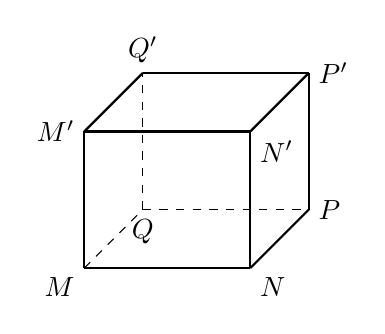
\begin{tikzpicture}[scale=0.62,>=stealth]
\draw[thick] (0,0)--(3.4,0);
\draw[thick] (3.4,0)--(4.6,1.2);
\draw[thick] (4.6,1.2)--(4.6,4.0);
\draw[thick] (0,2.8)--(3.4,2.8);
\draw[thick] (3.4,2.8)--(4.6,4.0);
\draw[thick] (4.6,4.0)--(1.2,4.0);
\draw[thick] (1.2,4.0)--(0,2.8);
\draw[thick] (0,0)--(0,2.8);
\draw[thick] (3.4,0)--(3.4,2.8);
\draw[dashed] (0,0)--(1.2,1.2);
\draw[dashed] (1.2,1.2)--(4.6,1.2);
\draw[dashed] (1.2,1.2)--(1.2,4.0);
\node[below left] at (0,0){$M$};
\node[below right] at (3.4,0){$N$};
\node[right] at (4.6,1.2){$P$};
\node[below] at (1.2,1.2){$Q$};
\node[left] at (0,2.8){$M'$};
\node[below right] at (3.4,2.8){$N'$};
\node[right] at (4.6,4.0){$P'$};
\node[above] at (1.2,4.0){$Q'$};
\end{tikzpicture}
\end{center}
Gọi $I$ là trung điểm của đoạn thẳng $QN'$.  Đặt $\vec{a}=\overrightarrow{MN}$, $\vec{b}=\overrightarrow{MQ}$, $\vec{c}=\overrightarrow{MM'}$. Biết $\overrightarrow{M'I}=x\vec{a}+y\vec{b}+z\vec{c}$. Bộ số $(x;y;z)$ là}
  {$(\dfrac{1}{2};\dfrac{1}{2};-\dfrac{1}{2})$.}
  {$(\dfrac{1}{2};-\dfrac{1}{2};\dfrac{1}{2})$.}{$(\dfrac{1}{2};\dfrac{1}{2};\dfrac{1}{2})$.}{$(-\dfrac{1}{2};\dfrac{1}{2};-\dfrac{1}{2})$.}

\cauTN[id=C2-B6-D01-VD-008,muc=VD,loigiai={Do $I$ là trung điểm nên $\overrightarrow{BI}=\dfrac{1}{2}(\overrightarrow{BS}+\overrightarrow{BC})$. Phân tích: $\overrightarrow{BS}=-\vec{b}$, $\overrightarrow{BC}=-\vec{b}+\vec{c}$. Cộng lại ta được $\overrightarrow{BI}=-\vec{b}+\dfrac{1}{2}\vec{c}$.}]{Cho tứ diện $SABC$. Gọi $I$ là trung điểm của đoạn thẳng $SC$. Đặt $\vec{a}=\overrightarrow{SA}$, $\vec{b}=\overrightarrow{SB}$, $\vec{c}=\overrightarrow{SC}$. Biết $\overrightarrow{BI}=x\vec{a}+y\vec{b}+z\vec{c}$. Bộ số $(x;y;z)$ là}
  {$(0;-1;\dfrac{1}{2})$.}
  {$(0;-1;\dfrac{5}{2})$.}{$(0;-1;0)$.}{$(-1;0;\dfrac{1}{2})$.}

\cauTN[id=C2-B6-D01-VD-009,muc=VD,loigiai={Do $I$ là trung điểm nên $\overrightarrow{AI}=\dfrac{1}{2}(\overrightarrow{AC}+\overrightarrow{AB})$. Phân tích: $\overrightarrow{AC}=\vec{a}+\vec{b}$, $\overrightarrow{AB}=\vec{a}$. Cộng lại ta được $\overrightarrow{AI}=\vec{a}+\dfrac{1}{2}\vec{b}$.}]{Cho hình chóp $S.ABCD$ có đáy $ABCD$ là hình bình hành. Gọi $I$ là trung điểm của đoạn thẳng $CB$. Đặt $\vec{a}=\overrightarrow{AB}$, $\vec{b}=\overrightarrow{AD}$, $\vec{c}=\overrightarrow{AS}$. Biết $\overrightarrow{AI}=x\vec{a}+y\vec{b}+z\vec{c}$. Bộ số $(x;y;z)$ là}
  {$(1;\dfrac{1}{2};0)$.}
  {$(1;0;\dfrac{1}{2})$.}{$(0;\dfrac{1}{2};1)$.}{$(2;\dfrac{1}{2};0)$.}

\cauTN[id=C2-B6-D01-VD-010,muc=VD,loigiai={Do $I$ là trung điểm nên $\overrightarrow{GI}=\dfrac{1}{2}(\overrightarrow{GF'}+\overrightarrow{GF})$. Phân tích: $\overrightarrow{GF'}=-\vec{b}+\vec{c}$, $\overrightarrow{GF}=-\vec{b}$. Cộng lại ta được $\overrightarrow{GI}=-\vec{b}+\dfrac{1}{2}\vec{c}$.}]{Cho hình hộp $EFGH.E'F'G'H'$ như hình vẽ.
\begin{center}
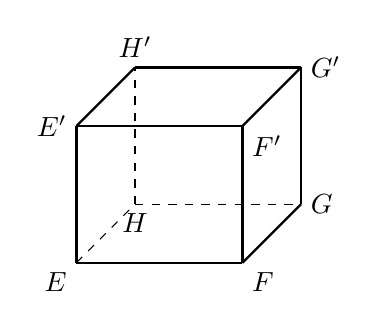
\begin{tikzpicture}[scale=0.62,>=stealth]
\draw[thick] (0,0)--(3.4,0);
\draw[thick] (3.4,0)--(4.6,1.2);
\draw[thick] (4.6,1.2)--(4.6,4.0);
\draw[thick] (0,2.8)--(3.4,2.8);
\draw[thick] (3.4,2.8)--(4.6,4.0);
\draw[thick] (4.6,4.0)--(1.2,4.0);
\draw[thick] (1.2,4.0)--(0,2.8);
\draw[thick] (0,0)--(0,2.8);
\draw[thick] (3.4,0)--(3.4,2.8);
\draw[dashed] (0,0)--(1.2,1.2);
\draw[dashed] (1.2,1.2)--(4.6,1.2);
\draw[dashed] (1.2,1.2)--(1.2,4.0);
\node[below left] at (0,0){$E$};
\node[below right] at (3.4,0){$F$};
\node[right] at (4.6,1.2){$G$};
\node[below] at (1.2,1.2){$H$};
\node[left] at (0,2.8){$E'$};
\node[below right] at (3.4,2.8){$F'$};
\node[right] at (4.6,4.0){$G'$};
\node[above] at (1.2,4.0){$H'$};
\end{tikzpicture}
\end{center}
Gọi $I$ là trung điểm của đoạn thẳng $F'F$.  Đặt $\vec{a}=\overrightarrow{EF}$, $\vec{b}=\overrightarrow{EH}$, $\vec{c}=\overrightarrow{EE'}$. Biết $\overrightarrow{GI}=x\vec{a}+y\vec{b}+z\vec{c}$. Bộ số $(x;y;z)$ là}
  {$(0;-1;\dfrac{1}{2})$.}
  {$(-1;-1;\dfrac{1}{2})$.}{$(-2;-1;\dfrac{1}{2})$.}{$(2;-1;\dfrac{1}{2})$.}

\cauTN[id=C2-B6-D01-VD-011,muc=VD,loigiai={Do $I$ là trung điểm nên $\overrightarrow{CI}=\dfrac{1}{2}(\overrightarrow{CS}+\overrightarrow{CA})$. Phân tích: $\overrightarrow{CS}=-\vec{c}$, $\overrightarrow{CA}=\vec{a}-\vec{c}$. Cộng lại ta được $\overrightarrow{CI}=\dfrac{1}{2}\vec{a}-\vec{c}$.}]{Cho tứ diện $SABC$. Gọi $I$ là trung điểm của đoạn thẳng $SA$. Đặt $\vec{a}=\overrightarrow{SA}$, $\vec{b}=\overrightarrow{SB}$, $\vec{c}=\overrightarrow{SC}$. Biết $\overrightarrow{CI}=x\vec{a}+y\vec{b}+z\vec{c}$. Bộ số $(x;y;z)$ là}
  {$(\dfrac{1}{2};0;-1)$.}
  {$(-\dfrac{1}{2};0;-1)$.}{$(\dfrac{1}{2};-2;-1)$.}{$(\dfrac{1}{2};2;-1)$.}

\cauTN[id=C2-B6-D01-VD-012,muc=VD,loigiai={Do $I$ là trung điểm nên $\overrightarrow{A'I}=\dfrac{1}{2}(\overrightarrow{A'D}+\overrightarrow{A'C'})$. Phân tích: $\overrightarrow{A'D}=\vec{b}-\vec{c}$, $\overrightarrow{A'C'}=\vec{a}+\vec{b}$. Cộng lại ta được $\overrightarrow{A'I}=\dfrac{1}{2}\vec{a}+\vec{b}-\dfrac{1}{2}\vec{c}$.}]{Cho hình hộp $ABCD.A'B'C'D'$. Gọi $I$ là trung điểm của đoạn thẳng $DC'$. Đặt $\vec{a}=\overrightarrow{AB}$, $\vec{b}=\overrightarrow{AD}$, $\vec{c}=\overrightarrow{AA'}$. Biết $\overrightarrow{A'I}=x\vec{a}+y\vec{b}+z\vec{c}$. Bộ số $(x;y;z)$ là}
  {$(\dfrac{1}{2};1;-\dfrac{1}{2})$.}
  {$(\dfrac{1}{2};3;-\dfrac{1}{2})$.}{$(1;\dfrac{1}{2};-\dfrac{1}{2})$.}{$(-\dfrac{3}{2};1;-\dfrac{1}{2})$.}

\cauTN[id=C2-B6-D01-VD-013,muc=VD,loigiai={Đặt $\vec a=\overrightarrow{AB}$, $\vec b=\overrightarrow{AD}$, $\vec c=\overrightarrow{AA'}$ đôi một vuông góc, $|\vec a|=2$, $|\vec b|=4$, $|\vec c|=3$. Ta có $\overrightarrow{C'G}+2\overrightarrow{BG}=-2\vec{a}+2\vec{b}$ nên $|\overrightarrow{C'G}+2\overrightarrow{BG}|^2=80$. Vậy $|\overrightarrow{C'G}+2\overrightarrow{BG}|=4\sqrt{5}$.}]{Cho hình hộp chữ nhật $ABCD.A'B'C'D'$ có $AB=2$, $AD=4$, $AA'=3$. Gọi $G$ là trọng tâm của tam giác $D'CD$. Gọi $I$ là trung điểm của đoạn thẳng $DB'$. Độ dài của vectơ $\overrightarrow{C'G}+2\overrightarrow{BG}$ bằng}
  {$4\sqrt{5}$.}
  {$\dfrac{4\sqrt{46}}{3}$.}{$\dfrac{\sqrt{217}}{3}$.}{$\dfrac{2\sqrt{217}}{3}$.}

\cauTN[id=C2-B6-D01-VD-014,muc=VD,loigiai={Đặt $\vec a=\overrightarrow{MN}$, $\vec b=\overrightarrow{MQ}$, $\vec c=\overrightarrow{MM'}$ đôi một vuông góc, $|\vec a|=6$, $|\vec b|=4$, $|\vec c|=12$. Ta có $\overrightarrow{NG}+\overrightarrow{QG}=\dfrac{1}{3}\vec{a}-\dfrac{1}{3}\vec{b}+2\vec{c}$ nên $|\overrightarrow{NG}+\overrightarrow{QG}|^2=\dfrac{5236}{9}$. Vậy $|\overrightarrow{NG}+\overrightarrow{QG}|=\dfrac{2\sqrt{1309}}{3}$.}]{Cho hình hộp chữ nhật $MNPQ.M'N'P'Q'$ có $MN=6$, $MQ=4$, $MM'=12$. Gọi $G$ là trọng tâm của tam giác $N'P'M'$. Gọi $H$ là trọng tâm của tam giác $QQ'M'$. Độ dài của vectơ $\overrightarrow{NG}+\overrightarrow{QG}$ bằng}
  {$\dfrac{2\sqrt{1309}}{3}$.}
  {$2\sqrt{13}$.}{$36$.}{$2\sqrt{337}$.}

\cauTN[id=C2-B6-D01-VD-015,muc=VD,loigiai={Đặt $\vec a=\overrightarrow{AB}$, $\vec b=\overrightarrow{AD}$, $\vec c=\overrightarrow{AE}$ đôi một vuông góc, $|\vec a|=4$, $|\vec b|=6$, $|\vec c|=4$. Ta có $\overrightarrow{IE}+\overrightarrow{GJ}=-\dfrac{3}{2}\vec{a}-2\vec{b}+\dfrac{1}{2}\vec{c}$ nên $|\overrightarrow{IE}+\overrightarrow{GJ}|^2=184$. Vậy $|\overrightarrow{IE}+\overrightarrow{GJ}|=2\sqrt{46}$.}]{Cho hình hộp chữ nhật $ABCD.EFGH$ có $AB=4$, $AD=6$, $AE=4$. Gọi $I$ là trung điểm của đoạn thẳng $CG$. Gọi $J$ là trung điểm của đoạn thẳng $EF$. Độ dài của vectơ $\overrightarrow{IE}+\overrightarrow{GJ}$ bằng}
  {$2\sqrt{46}$.}
  {$2\sqrt{110}$.}{$14\sqrt{2}$.}{$2\sqrt{2}$.}

\cauTN[id=C2-B6-D01-VD-016,muc=VD,loigiai={Đặt $\vec a=\overrightarrow{AB}$, $\vec b=\overrightarrow{AD}$, $\vec c=\overrightarrow{AE}$ đôi một vuông góc, $|\vec a|=4$, $|\vec b|=6$, $|\vec c|=4$. Ta có $\overrightarrow{JH}+\overrightarrow{CI}=-\dfrac{3}{2}\vec{a}+\vec{c}$ nên $|\overrightarrow{JH}+\overrightarrow{CI}|^2=52$. Vậy $|\overrightarrow{JH}+\overrightarrow{CI}|=2\sqrt{13}$.}]{Cho hình hộp chữ nhật $ABCD.EFGH$ có $AB=4$, $AD=6$, $AE=4$. Gọi $I$ là trung điểm của đoạn thẳng $AH$. Gọi $J$ là trung điểm của đoạn thẳng $EC$. Độ dài của vectơ $\overrightarrow{JH}+\overrightarrow{CI}$ bằng}
  {$2\sqrt{13}$.}
  {$\sqrt{145}$.}{$2\sqrt{10}$.}{$\sqrt{109}$.}

\cauTN[id=C2-B6-D01-VD-017,muc=VD,loigiai={Đặt $\vec a=\overrightarrow{EF}$, $\vec b=\overrightarrow{EH}$, $\vec c=\overrightarrow{EE'}$ đôi một vuông góc, $|\vec a|=6$, $|\vec b|=3$, $|\vec c|=3$. Ta có $-\overrightarrow{KH'}+\overrightarrow{JG'}=\dfrac{4}{3}\vec{a}-\dfrac{1}{3}\vec{b}-\dfrac{1}{3}\vec{c}$ nên $|-\overrightarrow{KH'}+\overrightarrow{JG'}|^2=66$. Vậy $|-\overrightarrow{KH'}+\overrightarrow{JG'}|=\sqrt{66}$.}]{Cho hình hộp chữ nhật $EFGH.E'F'G'H'$ có $EF=6$, $EH=3$, $EE'=3$. Gọi $J$ là trọng tâm của tam giác $E'GH'$. Gọi $K$ là trọng tâm của tam giác $EGF'$. Độ dài của vectơ $-\overrightarrow{KH'}+\overrightarrow{JG'}$ bằng}
  {$\sqrt{66}$.}
  {$9\sqrt{2}$.}{$12$.}{$3\sqrt{2}$.}

\cauTN[id=C2-B6-D01-VD-018,muc=VD,loigiai={Đặt $\vec a=\overrightarrow{EF}$, $\vec b=\overrightarrow{EH}$, $\vec c=\overrightarrow{EE'}$ đôi một vuông góc, $|\vec a|=6$, $|\vec b|=3$, $|\vec c|=6$. Ta có $\overrightarrow{GJ}+\overrightarrow{EI}=\dfrac{1}{6}\vec{a}-\dfrac{1}{6}\vec{b}+\dfrac{5}{6}\vec{c}$ nên $|\overrightarrow{GJ}+\overrightarrow{EI}|^2=\dfrac{105}{4}$. Vậy $|\overrightarrow{GJ}+\overrightarrow{EI}|=\dfrac{\sqrt{105}}{2}$.}]{Cho hình hộp chữ nhật $EFGH.E'F'G'H'$ có $EF=6$, $EH=3$, $EE'=6$. Gọi $J$ là trọng tâm của tam giác $G'EF$. Gọi $I$ là trung điểm của đoạn thẳng $G'E$. Độ dài của vectơ $\overrightarrow{GJ}+\overrightarrow{EI}$ bằng}
  {$\dfrac{\sqrt{105}}{2}$.}
  {$\dfrac{3\sqrt{17}}{2}$.}{$\dfrac{15}{2}$.}{$9$.}

\cauTN[id=C2-B6-D01-VD-019,muc=VD,loigiai={Đặt $\vec a=\overrightarrow{EF}$, $\vec b=\overrightarrow{EH}$, $\vec c=\overrightarrow{EE'}$ đôi một vuông góc, $|\vec a|=3$, $|\vec b|=12$, $|\vec c|=3$. Ta có $\overrightarrow{HJ}+\overrightarrow{JE'}=-\vec{b}+\vec{c}$ nên $|\overrightarrow{HJ}+\overrightarrow{JE'}|^2=153$. Vậy $|\overrightarrow{HJ}+\overrightarrow{JE'}|=3\sqrt{17}$.}]{Cho hình hộp chữ nhật $EFGH.E'F'G'H'$ có $EF=3$, $EH=12$, $EE'=3$. Gọi $J$ là trọng tâm của tam giác $H'GG'$. Gọi $K$ là trọng tâm của tam giác $H'EF$. Độ dài của vectơ $\overrightarrow{HJ}+\overrightarrow{JE'}$ bằng}
  {$3\sqrt{17}$.}
  {$\sqrt{161}$.}{$2\sqrt{149}$.}{$\sqrt{173}$.}

\cauTN[id=C2-B6-D01-VD-020,muc=VD,loigiai={Đặt $\vec a=\overrightarrow{AB}$, $\vec b=\overrightarrow{AD}$, $\vec c=\overrightarrow{AA'}$ đôi một vuông góc, $|\vec a|=3$, $|\vec b|=6$, $|\vec c|=2$. Ta có $\overrightarrow{IB'}+2\overrightarrow{B'G}=-\dfrac{5}{6}\vec{a}+\dfrac{4}{3}\vec{b}+\dfrac{1}{2}\vec{c}$ nên $|\overrightarrow{IB'}+2\overrightarrow{B'G}|^2=\dfrac{285}{4}$. Vậy $|\overrightarrow{IB'}+2\overrightarrow{B'G}|=\dfrac{\sqrt{285}}{2}$.}]{Cho hình hộp chữ nhật $ABCD.A'B'C'D'$ có $AB=3$, $AD=6$, $AA'=2$. Gọi $I$ là trung điểm của đoạn thẳng $BA'$. Gọi $G$ là trọng tâm của tam giác $A'C'D'$. Độ dài của vectơ $\overrightarrow{IB'}+2\overrightarrow{B'G}$ bằng}
  {$\dfrac{\sqrt{285}}{2}$.}
  {$\dfrac{\sqrt{381}}{2}$.}{$\sqrt{69}$.}{$\dfrac{\sqrt{69}}{2}$.}

\cauTN[id=C2-B6-D01-VD-021,muc=VD,loigiai={Đặt $\vec a=\overrightarrow{EF}$, $\vec b=\overrightarrow{EH}$, $\vec c=\overrightarrow{EE'}$ đôi một vuông góc, $|\vec a|=12$, $|\vec b|=6$, $|\vec c|=3$. Ta có $2\overrightarrow{GI}+\overrightarrow{F'I}=-\dfrac{3}{2}\vec{a}-\dfrac{1}{2}\vec{b}+\dfrac{1}{2}\vec{c}$ nên $|2\overrightarrow{GI}+\overrightarrow{F'I}|^2=\dfrac{1341}{4}$. Vậy $|2\overrightarrow{GI}+\overrightarrow{F'I}|=\dfrac{3\sqrt{149}}{2}$.}]{Cho hình hộp chữ nhật $EFGH.E'F'G'H'$ có $EF=12$, $EH=6$, $EE'=3$. Gọi $J$ là trọng tâm của tam giác $EE'F'$. Gọi $I$ là trung điểm của đoạn thẳng $F'H$. Độ dài của vectơ $2\overrightarrow{GI}+\overrightarrow{F'I}$ bằng}
  {$\dfrac{3\sqrt{149}}{2}$.}
  {$\dfrac{3\sqrt{61}}{2}$.}{$24$.}{$12$.}

\cauTN[id=C2-B6-D01-VD-022,muc=VD,loigiai={Đặt $\vec a=\overrightarrow{AB}$, $\vec b=\overrightarrow{AD}$, $\vec c=\overrightarrow{AA'}$ đôi một vuông góc, $|\vec a|=2$, $|\vec b|=4$, $|\vec c|=2$. Ta có $\overrightarrow{GC}+\overrightarrow{A'H}=\dfrac{1}{3}\vec{a}+\vec{b}-\vec{c}$ nên $|\overrightarrow{GC}+\overrightarrow{A'H}|^2=\dfrac{184}{9}$. Vậy $|\overrightarrow{GC}+\overrightarrow{A'H}|=\dfrac{2\sqrt{46}}{3}$.}]{Cho hình hộp chữ nhật $ABCD.A'B'C'D'$ có $AB=2$, $AD=4$, $AA'=2$. Gọi $G$ là trọng tâm của tam giác $BB'C$. Gọi $H$ là trọng tâm của tam giác $A'DB$. Độ dài của vectơ $\overrightarrow{GC}+\overrightarrow{A'H}$ bằng}
  {$\dfrac{2\sqrt{46}}{3}$.}
  {$\dfrac{2\sqrt{93}}{3}$.}{$2\sqrt{13}$.}{$\dfrac{2\sqrt{6}}{3}$.}

\cauTN[id=C2-B6-D01-VD-023,muc=VD,loigiai={Đặt $\vec a=\overrightarrow{MN}$, $\vec b=\overrightarrow{MQ}$, $\vec c=\overrightarrow{MM'}$ đôi một vuông góc, $|\vec a|=4$, $|\vec b|=2$, $|\vec c|=2$. Ta có $\overrightarrow{N'I}-\overrightarrow{NG}=-\dfrac{2}{3}\vec{a}-\dfrac{1}{3}\vec{b}-\dfrac{7}{6}\vec{c}$ nên $|\overrightarrow{N'I}-\overrightarrow{NG}|^2=13$. Vậy $|\overrightarrow{N'I}-\overrightarrow{NG}|=\sqrt{13}$.}]{Cho hình hộp chữ nhật $MNPQ.M'N'P'Q'$ có $MN=4$, $MQ=2$, $MM'=2$. Gọi $I$ là trung điểm của đoạn thẳng $M'M$. Gọi $G$ là trọng tâm của tam giác $Q'NN'$. Độ dài của vectơ $\overrightarrow{N'I}-\overrightarrow{NG}$ bằng}
  {$\sqrt{13}$.}
  {$\sqrt{29}$.}{$2\sqrt{14}$.}{$\sqrt{17}$.}

\cauTN[id=C2-B6-D01-VD-024,muc=VD,loigiai={Đặt $\vec a=\overrightarrow{EF}$, $\vec b=\overrightarrow{EH}$, $\vec c=\overrightarrow{EE'}$ đôi một vuông góc, $|\vec a|=12$, $|\vec b|=12$, $|\vec c|=12$. Ta có $2\overrightarrow{E'I}+\overrightarrow{H'I}=\dfrac{3}{2}\vec{a}+2\vec{b}$ nên $|2\overrightarrow{E'I}+\overrightarrow{H'I}|^2=900$. Vậy $|2\overrightarrow{E'I}+\overrightarrow{H'I}|=30$.}]{Cho hình hộp chữ nhật $EFGH.E'F'G'H'$ có $EF=12$, $EH=12$, $EE'=12$. Gọi $I$ là trung điểm của đoạn thẳng $H'G'$. Gọi $J$ là trung điểm của đoạn thẳng $FG$. Độ dài của vectơ $2\overrightarrow{E'I}+\overrightarrow{H'I}$ bằng}
  {$30$.}
  {$6\sqrt{17}$.}{$24\sqrt{2}$.}{$12\sqrt{2}$.}

\cauTN[id=C2-B6-D01-VD-025,muc=VD,loigiai={Từ $3\overrightarrow{IS}+2\overrightarrow{ID}=\overrightarrow{0}$ suy ra $3\overrightarrow{IS}+2(\overrightarrow{IS}+\overrightarrow{SD})=\overrightarrow{0}$, tức là $5\,\overrightarrow{SI}=2\,\overrightarrow{SD}$. Do đó $\overrightarrow{SI}=\dfrac{2}{5}\overrightarrow{SD}$ và $x=\dfrac{2}{5}$.}]{Cho hình chóp $S.ABCD$ có đáy $ABCD$ là hình bình hành như hình vẽ.
\begin{center}
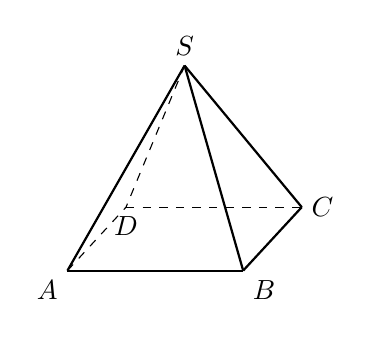
\begin{tikzpicture}[scale=0.62,>=stealth]
\draw[thick] (0,0)--(3.6,0);
\draw[thick] (3.6,0)--(4.8,1.3);
\draw[thick] (2.4,4.2)--(0,0);
\draw[thick] (2.4,4.2)--(3.6,0);
\draw[thick] (2.4,4.2)--(4.8,1.3);
\draw[dashed] (0,0)--(1.2,1.3);
\draw[dashed] (1.2,1.3)--(4.8,1.3);
\draw[dashed] (2.4,4.2)--(1.2,1.3);
\node[below left] at (0,0){$A$};
\node[below right] at (3.6,0){$B$};
\node[right] at (4.8,1.3){$C$};
\node[below] at (1.2,1.3){$D$};
\node[above] at (2.4,4.2){$S$};
\end{tikzpicture}
\end{center}
Gọi $I$ là điểm thoả mãn $3\overrightarrow{IS}+2\overrightarrow{ID}=\overrightarrow{0}$.  Biết $\overrightarrow{SI}=x\,\overrightarrow{SD}$. Giá trị của $x$ bằng}
  {$\dfrac{2}{5}$.}
  {$\dfrac{3}{5}$.}{$\dfrac{2}{3}$.}{$\dfrac{5}{2}$.}

\cauTN[id=C2-B6-D01-VD-026,muc=VD,loigiai={Từ $\overrightarrow{IC}+\overrightarrow{IH}-\overrightarrow{IG}=\overrightarrow{0}$, với điểm $M$ bất kì: $\overrightarrow{MC}+\overrightarrow{MH}-\overrightarrow{MG}=(1+1-1)\overrightarrow{MI}$ nên $\overrightarrow{MC}+\overrightarrow{MH}-\overrightarrow{MG}=(1+1-1)\,\overrightarrow{MI}$. Vậy $k=1$.}]{Cho hình hộp $ABCD.EFGH$. Gọi $I$ là điểm thoả mãn $\overrightarrow{IC}+\overrightarrow{IH}-\overrightarrow{IG}=\overrightarrow{0}$. Với mọi điểm $M$, ta có $\overrightarrow{MC}+\overrightarrow{MH}-\overrightarrow{MG}=k\,\overrightarrow{MI}$. Giá trị của $k$ bằng}
  {$1$.}
  {$2$.}{$-1$.}{$3$.}

\cauTN[id=C2-B6-D01-VD-027,muc=VD,loigiai={Từ $3\overrightarrow{IF}+\overrightarrow{IA}-\overrightarrow{IH}=\overrightarrow{0}$, với điểm $M$ bất kì: $3\overrightarrow{MF}+\overrightarrow{MA}-\overrightarrow{MH}=(3+1-1)\overrightarrow{MI}$ nên $3\overrightarrow{MF}+\overrightarrow{MA}-\overrightarrow{MH}=(3+1-1)\,\overrightarrow{MI}$. Vậy $k=3$.}]{Cho hình hộp $ABCD.EFGH$. Gọi $I$ là điểm thoả mãn $3\overrightarrow{IF}+\overrightarrow{IA}-\overrightarrow{IH}=\overrightarrow{0}$. Với mọi điểm $M$, ta có $3\overrightarrow{MF}+\overrightarrow{MA}-\overrightarrow{MH}=k\,\overrightarrow{MI}$. Giá trị của $k$ bằng}
  {$3$.}
  {$2$.}{$4$.}{$-3$.}

\cauTN[id=C2-B6-D01-VD-028,muc=VD,loigiai={Từ $3\overrightarrow{ID}+2\overrightarrow{IB}=\overrightarrow{0}$ suy ra $3\overrightarrow{ID}+2(\overrightarrow{ID}+\overrightarrow{DB})=\overrightarrow{0}$, tức là $5\,\overrightarrow{DI}=2\,\overrightarrow{DB}$. Do đó $\overrightarrow{DI}=\dfrac{2}{5}\overrightarrow{DB}$ và $x=\dfrac{2}{5}$.}]{Cho hình chóp $O.ABCD$ có đáy $ABCD$ là hình bình hành như hình vẽ.
\begin{center}
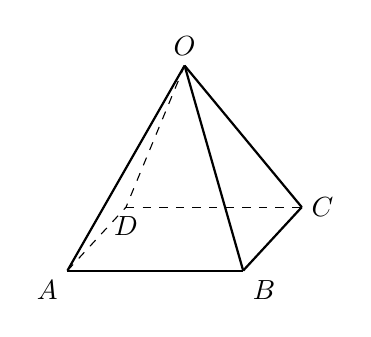
\begin{tikzpicture}[scale=0.62,>=stealth]
\draw[thick] (0,0)--(3.6,0);
\draw[thick] (3.6,0)--(4.8,1.3);
\draw[thick] (2.4,4.2)--(0,0);
\draw[thick] (2.4,4.2)--(3.6,0);
\draw[thick] (2.4,4.2)--(4.8,1.3);
\draw[dashed] (0,0)--(1.2,1.3);
\draw[dashed] (1.2,1.3)--(4.8,1.3);
\draw[dashed] (2.4,4.2)--(1.2,1.3);
\node[below left] at (0,0){$A$};
\node[below right] at (3.6,0){$B$};
\node[right] at (4.8,1.3){$C$};
\node[below] at (1.2,1.3){$D$};
\node[above] at (2.4,4.2){$O$};
\end{tikzpicture}
\end{center}
Gọi $I$ là điểm thoả mãn $3\overrightarrow{ID}+2\overrightarrow{IB}=\overrightarrow{0}$.  Biết $\overrightarrow{DI}=x\,\overrightarrow{DB}$. Giá trị của $x$ bằng}
  {$\dfrac{2}{5}$.}
  {$\dfrac{3}{5}$.}{$\dfrac{2}{3}$.}{$\dfrac{5}{2}$.}

\cauTN[id=C2-B6-D01-VD-029,muc=VD,loigiai={Từ $2\overrightarrow{IM}-\overrightarrow{IS}=\overrightarrow{0}$ suy ra $2\overrightarrow{IM}-1(\overrightarrow{IM}+\overrightarrow{MS})=\overrightarrow{0}$, tức là $\,\overrightarrow{MI}=-1\,\overrightarrow{MS}$. Do đó $\overrightarrow{MI}=\dfrac{-1}{1}\overrightarrow{MS}$ và $x=-1$.}]{Cho hình chóp $S.MNPQ$ có đáy $MNPQ$ là hình bình hành như hình vẽ.
\begin{center}
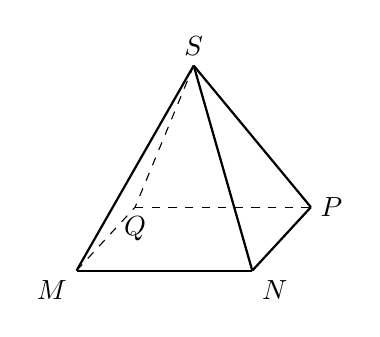
\begin{tikzpicture}[scale=0.62,>=stealth]
\draw[thick] (0,0)--(3.6,0);
\draw[thick] (3.6,0)--(4.8,1.3);
\draw[thick] (2.4,4.2)--(0,0);
\draw[thick] (2.4,4.2)--(3.6,0);
\draw[thick] (2.4,4.2)--(4.8,1.3);
\draw[dashed] (0,0)--(1.2,1.3);
\draw[dashed] (1.2,1.3)--(4.8,1.3);
\draw[dashed] (2.4,4.2)--(1.2,1.3);
\node[below left] at (0,0){$M$};
\node[below right] at (3.6,0){$N$};
\node[right] at (4.8,1.3){$P$};
\node[below] at (1.2,1.3){$Q$};
\node[above] at (2.4,4.2){$S$};
\end{tikzpicture}
\end{center}
Gọi $I$ là điểm thoả mãn $2\overrightarrow{IM}-\overrightarrow{IS}=\overrightarrow{0}$.  Biết $\overrightarrow{MI}=x\,\overrightarrow{MS}$. Giá trị của $x$ bằng}
  {$-1$.}
  {$2$.}{$-\dfrac{1}{2}$.}{$1$.}

\cauTN[id=C2-B6-D01-VD-030,muc=VD,loigiai={Từ $\overrightarrow{ID}-\overrightarrow{IG}+\overrightarrow{IA}+3\overrightarrow{IF}=\overrightarrow{0}$, với điểm $M$ bất kì: $\overrightarrow{MD}-\overrightarrow{MG}+\overrightarrow{MA}+3\overrightarrow{MF}=(1-1+1+3)\overrightarrow{MI}$ nên $\overrightarrow{MD}-\overrightarrow{MG}+\overrightarrow{MA}+3\overrightarrow{MF}=(1-1+1+3)\,\overrightarrow{MI}$. Vậy $k=4$.}]{Cho hình hộp $ABCD.EFGH$. Gọi $I$ là điểm thoả mãn $\overrightarrow{ID}-\overrightarrow{IG}+\overrightarrow{IA}+3\overrightarrow{IF}=\overrightarrow{0}$. Với mọi điểm $M$, ta có $\overrightarrow{MD}-\overrightarrow{MG}+\overrightarrow{MA}+3\overrightarrow{MF}=k\,\overrightarrow{MI}$. Giá trị của $k$ bằng}
  {$4$.}
  {$3$.}{$5$.}{$-4$.}

\cauTN[id=C2-B6-D01-VD-031,muc=VD,loigiai={Từ $3\overrightarrow{IF}+\overrightarrow{IE}-\overrightarrow{IG'}=\overrightarrow{0}$, với điểm $M$ bất kì: $3\overrightarrow{MF}+\overrightarrow{ME}-\overrightarrow{MG'}=(3+1-1)\overrightarrow{MI}$ nên $3\overrightarrow{MF}+\overrightarrow{ME}-\overrightarrow{MG'}=(3+1-1)\,\overrightarrow{MI}$. Vậy $k=3$.}]{Cho hình hộp $EFGH.E'F'G'H'$. Gọi $I$ là điểm thoả mãn $3\overrightarrow{IF}+\overrightarrow{IE}-\overrightarrow{IG'}=\overrightarrow{0}$. Với mọi điểm $M$, ta có $3\overrightarrow{MF}+\overrightarrow{ME}-\overrightarrow{MG'}=k\,\overrightarrow{MI}$. Giá trị của $k$ bằng}
  {$3$.}
  {$2$.}{$4$.}{$-3$.}

\cauTN[id=C2-B6-D01-VD-032,muc=VD,loigiai={Từ $\overrightarrow{IP'}+3\overrightarrow{IQ}=\overrightarrow{0}$ suy ra $1\overrightarrow{IP'}+3(\overrightarrow{IP'}+\overrightarrow{P'Q})=\overrightarrow{0}$, tức là $4\,\overrightarrow{P'I}=3\,\overrightarrow{P'Q}$. Do đó $\overrightarrow{P'I}=\dfrac{3}{4}\overrightarrow{P'Q}$ và $x=\dfrac{3}{4}$.}]{Cho hình hộp $MNPQ.M'N'P'Q'$ như hình vẽ.
\begin{center}
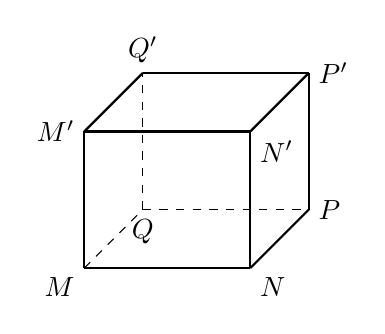
\begin{tikzpicture}[scale=0.62,>=stealth]
\draw[thick] (0,0)--(3.4,0);
\draw[thick] (3.4,0)--(4.6,1.2);
\draw[thick] (4.6,1.2)--(4.6,4.0);
\draw[thick] (0,2.8)--(3.4,2.8);
\draw[thick] (3.4,2.8)--(4.6,4.0);
\draw[thick] (4.6,4.0)--(1.2,4.0);
\draw[thick] (1.2,4.0)--(0,2.8);
\draw[thick] (0,0)--(0,2.8);
\draw[thick] (3.4,0)--(3.4,2.8);
\draw[dashed] (0,0)--(1.2,1.2);
\draw[dashed] (1.2,1.2)--(4.6,1.2);
\draw[dashed] (1.2,1.2)--(1.2,4.0);
\node[below left] at (0,0){$M$};
\node[below right] at (3.4,0){$N$};
\node[right] at (4.6,1.2){$P$};
\node[below] at (1.2,1.2){$Q$};
\node[left] at (0,2.8){$M'$};
\node[below right] at (3.4,2.8){$N'$};
\node[right] at (4.6,4.0){$P'$};
\node[above] at (1.2,4.0){$Q'$};
\end{tikzpicture}
\end{center}
Gọi $I$ là điểm thoả mãn $\overrightarrow{IP'}+3\overrightarrow{IQ}=\overrightarrow{0}$.  Biết $\overrightarrow{P'I}=x\,\overrightarrow{P'Q}$. Giá trị của $x$ bằng}
  {$\dfrac{3}{4}$.}
  {$\dfrac{1}{4}$.}{$3$.}{$\dfrac{4}{3}$.}

\cauTN[id=C2-B6-D01-VD-033,muc=VD,loigiai={Từ $3\overrightarrow{ID}+\overrightarrow{IB}+2\overrightarrow{IA}=\overrightarrow{0}$, với điểm $M$ bất kì: $3\overrightarrow{MD}+\overrightarrow{MB}+2\overrightarrow{MA}=(3+1+2)\overrightarrow{MI}$ nên $3\overrightarrow{MD}+\overrightarrow{MB}+2\overrightarrow{MA}=(3+1+2)\,\overrightarrow{MI}$. Vậy $k=6$.}]{Cho hình hộp $ABCD.A'B'C'D'$. Gọi $I$ là điểm thoả mãn $3\overrightarrow{ID}+\overrightarrow{IB}+2\overrightarrow{IA}=\overrightarrow{0}$. Với mọi điểm $M$, ta có $3\overrightarrow{MD}+\overrightarrow{MB}+2\overrightarrow{MA}=k\,\overrightarrow{MI}$. Giá trị của $k$ bằng}
  {$6$.}
  {$5$.}{$7$.}{$-6$.}

\cauTN[id=C2-B6-D01-VD-034,muc=VD,loigiai={Từ $3\overrightarrow{IE'}-\overrightarrow{IF'}=\overrightarrow{0}$ suy ra $3\overrightarrow{IE'}-1(\overrightarrow{IE'}+\overrightarrow{E'F'})=\overrightarrow{0}$, tức là $2\,\overrightarrow{E'I}=-1\,\overrightarrow{E'F'}$. Do đó $\overrightarrow{E'I}=\dfrac{-1}{2}\overrightarrow{E'F'}$ và $x=-\dfrac{1}{2}$.}]{Cho hình hộp $EFGH.E'F'G'H'$. Gọi $I$ là điểm thoả mãn $3\overrightarrow{IE'}-\overrightarrow{IF'}=\overrightarrow{0}$. Biết $\overrightarrow{E'I}=x\,\overrightarrow{E'F'}$. Giá trị của $x$ bằng}
  {$-\dfrac{1}{2}$.}
  {$\dfrac{3}{2}$.}{$-\dfrac{1}{3}$.}{$-2$.}

\cauTN[id=C2-B6-D01-VD-035,muc=VD,loigiai={Từ $3\overrightarrow{ID}+2\overrightarrow{IA}+\overrightarrow{IC}=\overrightarrow{0}$, với điểm $M$ bất kì: $3\overrightarrow{MD}+2\overrightarrow{MA}+\overrightarrow{MC}=(3+2+1)\overrightarrow{MI}$ nên $3\overrightarrow{MD}+2\overrightarrow{MA}+\overrightarrow{MC}=(3+2+1)\,\overrightarrow{MI}$. Vậy $k=6$.}]{Cho hình chóp $S.ABCD$ có đáy $ABCD$ là hình bình hành. Gọi $I$ là điểm thoả mãn $3\overrightarrow{ID}+2\overrightarrow{IA}+\overrightarrow{IC}=\overrightarrow{0}$. Với mọi điểm $M$, ta có $3\overrightarrow{MD}+2\overrightarrow{MA}+\overrightarrow{MC}=k\,\overrightarrow{MI}$. Giá trị của $k$ bằng}
  {$6$.}
  {$5$.}{$7$.}{$-6$.}

\cauTN[id=C2-B6-D01-VD-036,muc=VD,loigiai={Từ $3\overrightarrow{IP}-\overrightarrow{IM}=\overrightarrow{0}$ suy ra $3\overrightarrow{IP}-1(\overrightarrow{IP}+\overrightarrow{PM})=\overrightarrow{0}$, tức là $2\,\overrightarrow{PI}=-1\,\overrightarrow{PM}$. Do đó $\overrightarrow{PI}=\dfrac{-1}{2}\overrightarrow{PM}$ và $x=-\dfrac{1}{2}$.}]{Cho tứ diện $MNPQ$. Gọi $I$ là điểm thoả mãn $3\overrightarrow{IP}-\overrightarrow{IM}=\overrightarrow{0}$. Biết $\overrightarrow{PI}=x\,\overrightarrow{PM}$. Giá trị của $x$ bằng}
  {$-\dfrac{1}{2}$.}
  {$\dfrac{3}{2}$.}{$-\dfrac{1}{3}$.}{$-2$.}

\cauDS[id=C2-B6-D01-VD-037,muc=VD,loigiai={Từ $\sum w_i\overrightarrow{IA_i}=\overrightarrow{0}$ suy ra với mọi điểm $M$: $\sum w_i\overrightarrow{MA_i}=4\,\overrightarrow{MI}$; đồng thời biểu diễn $\overrightarrow{BI}$ theo các vectơ gốc $B$. a) Đúng. b) Đúng. c) Sai. d) Sai.}]{Cho tứ diện $ABCD$. Gọi $I$ là điểm thoả mãn $-\overrightarrow{IB}+2\overrightarrow{IC}+3\overrightarrow{IA}=\overrightarrow{0}$. Xét tính đúng sai của các mệnh đề sau:}{%
  \y{$-\overrightarrow{MB}+2\overrightarrow{MC}+3\overrightarrow{MA}=4\overrightarrow{MI}$.}{d}
  \y{$\overrightarrow{BI}=\dfrac{1}{2}\overrightarrow{BC}+\dfrac{3}{4}\overrightarrow{BA}$.}{d}
  \y{$-\overrightarrow{IB}+2\overrightarrow{IC}+4\overrightarrow{IA}=\overrightarrow{0}$.}{s}
  \y{$-\overrightarrow{IB}+3\overrightarrow{IC}+3\overrightarrow{IA}=\overrightarrow{0}$.}{s}}

\cauDS[id=C2-B6-D01-VD-038,muc=VD,loigiai={Từ $\sum w_i\overrightarrow{IA_i}=\overrightarrow{0}$ suy ra với mọi điểm $M$: $\sum w_i\overrightarrow{MA_i}=1\,\overrightarrow{MI}$; đồng thời biểu diễn $\overrightarrow{BI}$ theo các vectơ gốc $B$. a) Đúng. b) Sai. c) Sai. d) Đúng.}]{Cho hình chóp $O.ABCD$ có đáy $ABCD$ là hình bình hành. Gọi $I$ là điểm thoả mãn $-\overrightarrow{IB}+2\overrightarrow{IC}=\overrightarrow{0}$. Xét tính đúng sai của các mệnh đề sau:}{%
  \y{$\overrightarrow{IC}=-\overrightarrow{BC}$.}{d}
  \y{$-\overrightarrow{MB}+2\overrightarrow{MC}=0\overrightarrow{MI}$.}{s}
  \y{$0\overrightarrow{IB}+2\overrightarrow{IC}=\overrightarrow{0}$.}{s}
  \y{$\overrightarrow{BI}=2\overrightarrow{BC}$.}{d}}

\cauDS[id=C2-B6-D01-VD-039,muc=VD,loigiai={Từ $\sum w_i\overrightarrow{IA_i}=\overrightarrow{0}$ suy ra với mọi điểm $M$: $\sum w_i\overrightarrow{MA_i}=3\,\overrightarrow{MI}$; đồng thời biểu diễn $\overrightarrow{A'I}$ theo các vectơ gốc $A'$. a) Đúng. b) Sai. c) Đúng. d) Sai.}]{Cho hình hộp $ABCD.A'B'C'D'$ như hình vẽ.
\begin{center}
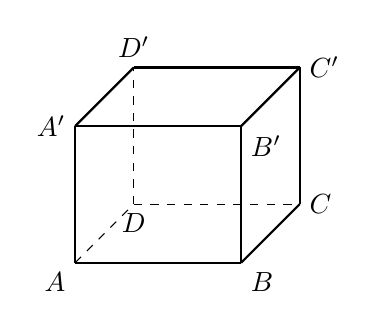
\begin{tikzpicture}[scale=0.62,>=stealth]
\draw[thick] (0,0)--(3.4,0);
\draw[thick] (3.4,0)--(4.6,1.2);
\draw[thick] (4.6,1.2)--(4.6,4.0);
\draw[thick] (0,2.8)--(3.4,2.8);
\draw[thick] (3.4,2.8)--(4.6,4.0);
\draw[thick] (4.6,4.0)--(1.2,4.0);
\draw[thick] (1.2,4.0)--(0,2.8);
\draw[thick] (0,0)--(0,2.8);
\draw[thick] (3.4,0)--(3.4,2.8);
\draw[dashed] (0,0)--(1.2,1.2);
\draw[dashed] (1.2,1.2)--(4.6,1.2);
\draw[dashed] (1.2,1.2)--(1.2,4.0);
\node[below left] at (0,0){$A$};
\node[below right] at (3.4,0){$B$};
\node[right] at (4.6,1.2){$C$};
\node[below] at (1.2,1.2){$D$};
\node[left] at (0,2.8){$A'$};
\node[below right] at (3.4,2.8){$B'$};
\node[right] at (4.6,4.0){$C'$};
\node[above] at (1.2,4.0){$D'$};
\end{tikzpicture}
\end{center}
Gọi $I$ là điểm thoả mãn $-\overrightarrow{IA'}+2\overrightarrow{ID}+2\overrightarrow{ID'}=\overrightarrow{0}$.  Xét tính đúng sai của các mệnh đề sau:}{%
  \y{$-\overrightarrow{MA'}+2\overrightarrow{MD}+2\overrightarrow{MD'}=3\overrightarrow{MI}$.}{d}
  \y{$\overrightarrow{IA'}+2\overrightarrow{ID}+2\overrightarrow{ID'}=\overrightarrow{0}$.}{s}
  \y{$\overrightarrow{A'I}=\dfrac{2}{3}\overrightarrow{A'D}+\dfrac{2}{3}\overrightarrow{A'D'}$.}{d}
  \y{$-\overrightarrow{MA'}+2\overrightarrow{MD}+2\overrightarrow{MD'}=2\overrightarrow{MI}$.}{s}}

\cauDS[id=C2-B6-D01-VD-040,muc=VD,loigiai={Từ $\sum w_i\overrightarrow{IA_i}=\overrightarrow{0}$ suy ra với mọi điểm $M$: $\sum w_i\overrightarrow{MA_i}=-1\,\overrightarrow{MI}$; đồng thời biểu diễn $\overrightarrow{HI}$ theo các vectơ gốc $H$. a) Sai. b) Đúng. c) Sai. d) Đúng.}]{Cho hình hộp $ABCD.EFGH$ như hình vẽ.
\begin{center}
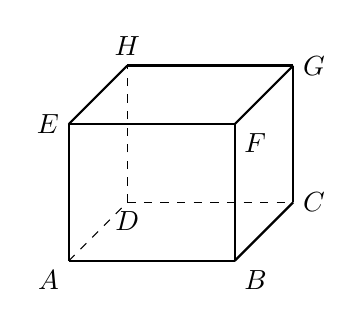
\begin{tikzpicture}[scale=0.62,>=stealth]
\draw[thick] (0,0)--(3.4,0);
\draw[thick] (3.4,0)--(4.6,1.2);
\draw[thick] (4.6,1.2)--(4.6,4.0);
\draw[thick] (0,2.8)--(3.4,2.8);
\draw[thick] (3.4,2.8)--(4.6,4.0);
\draw[thick] (4.6,4.0)--(1.2,4.0);
\draw[thick] (1.2,4.0)--(0,2.8);
\draw[thick] (0,0)--(0,2.8);
\draw[thick] (3.4,0)--(3.4,2.8);
\draw[dashed] (0,0)--(1.2,1.2);
\draw[dashed] (1.2,1.2)--(4.6,1.2);
\draw[dashed] (1.2,1.2)--(1.2,4.0);
\node[below left] at (0,0){$A$};
\node[below right] at (3.4,0){$B$};
\node[right] at (4.6,1.2){$C$};
\node[below] at (1.2,1.2){$D$};
\node[left] at (0,2.8){$E$};
\node[below right] at (3.4,2.8){$F$};
\node[right] at (4.6,4.0){$G$};
\node[above] at (1.2,4.0){$H$};
\end{tikzpicture}
\end{center}
Gọi $I$ là điểm thoả mãn $-\overrightarrow{IH}-\overrightarrow{IG}+\overrightarrow{IC}=\overrightarrow{0}$.  Xét tính đúng sai của các mệnh đề sau:}{%
  \y{$-\overrightarrow{IH}-\overrightarrow{IG}+0\overrightarrow{IC}=\overrightarrow{0}$.}{s}
  \y{$\overrightarrow{HI}=\overrightarrow{HG}-\overrightarrow{HC}$.}{d}
  \y{$\overrightarrow{IH}-\overrightarrow{IG}+\overrightarrow{IC}=\overrightarrow{0}$.}{s}
  \y{$-\overrightarrow{MH}-\overrightarrow{MG}+\overrightarrow{MC}=-\overrightarrow{MI}$.}{d}}

\cauDS[id=C2-B6-D01-VD-041,muc=VD,loigiai={Từ $\sum w_i\overrightarrow{IA_i}=\overrightarrow{0}$ suy ra với mọi điểm $O$: $\sum w_i\overrightarrow{OA_i}=3\,\overrightarrow{OI}$; đồng thời biểu diễn $\overrightarrow{PI}$ theo các vectơ gốc $P$. a) Sai. b) Sai. c) Sai. d) Đúng.}]{Cho hình hộp $MNPQ.M'N'P'Q'$ như hình vẽ.
\begin{center}
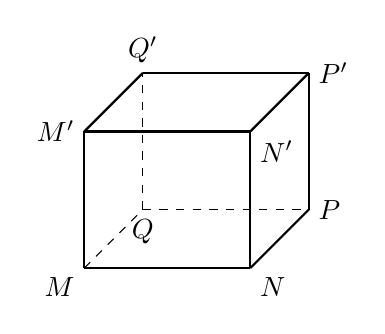
\begin{tikzpicture}[scale=0.62,>=stealth]
\draw[thick] (0,0)--(3.4,0);
\draw[thick] (3.4,0)--(4.6,1.2);
\draw[thick] (4.6,1.2)--(4.6,4.0);
\draw[thick] (0,2.8)--(3.4,2.8);
\draw[thick] (3.4,2.8)--(4.6,4.0);
\draw[thick] (4.6,4.0)--(1.2,4.0);
\draw[thick] (1.2,4.0)--(0,2.8);
\draw[thick] (0,0)--(0,2.8);
\draw[thick] (3.4,0)--(3.4,2.8);
\draw[dashed] (0,0)--(1.2,1.2);
\draw[dashed] (1.2,1.2)--(4.6,1.2);
\draw[dashed] (1.2,1.2)--(1.2,4.0);
\node[below left] at (0,0){$M$};
\node[below right] at (3.4,0){$N$};
\node[right] at (4.6,1.2){$P$};
\node[below] at (1.2,1.2){$Q$};
\node[left] at (0,2.8){$M'$};
\node[below right] at (3.4,2.8){$N'$};
\node[right] at (4.6,4.0){$P'$};
\node[above] at (1.2,4.0){$Q'$};
\end{tikzpicture}
\end{center}
Gọi $I$ là điểm thoả mãn $\overrightarrow{IP}+2\overrightarrow{IQ}=\overrightarrow{0}$.  Xét tính đúng sai của các mệnh đề sau:}{%
  \y{$\overrightarrow{PI}=\dfrac{1}{3}\overrightarrow{PQ}$.}{s}
  \y{$\overrightarrow{IP}+4\overrightarrow{IQ}=\overrightarrow{0}$.}{s}
  \y{$\overrightarrow{IQ}=\dfrac{2}{3}\overrightarrow{PQ}$.}{s}
  \y{$\overrightarrow{OP}+2\overrightarrow{OQ}=3\overrightarrow{OI}$.}{d}}

\cauDS[id=C2-B6-D01-VD-042,muc=VD,loigiai={Từ $\sum w_i\overrightarrow{IA_i}=\overrightarrow{0}$ suy ra với mọi điểm $M$: $\sum w_i\overrightarrow{MA_i}=3\,\overrightarrow{MI}$; đồng thời biểu diễn $\overrightarrow{G'I}$ theo các vectơ gốc $G'$. a) Sai. b) Đúng. c) Đúng. d) Đúng.}]{Cho hình hộp $EFGH.E'F'G'H'$. Gọi $I$ là điểm thoả mãn $\overrightarrow{IG'}+2\overrightarrow{IG}=\overrightarrow{0}$. Xét tính đúng sai của các mệnh đề sau:}{%
  \y{$2\overrightarrow{IG'}+2\overrightarrow{IG}=\overrightarrow{0}$.}{s}
  \y{$\overrightarrow{IG}=\dfrac{1}{3}\overrightarrow{G'G}$.}{d}
  \y{$\overrightarrow{MG'}+2\overrightarrow{MG}=3\overrightarrow{MI}$.}{d}
  \y{$\overrightarrow{G'I}=\dfrac{2}{3}\overrightarrow{G'G}$.}{d}}

\cauDS[id=C2-B6-D01-VD-043,muc=VD,loigiai={Từ $\sum w_i\overrightarrow{IA_i}=\overrightarrow{0}$ suy ra với mọi điểm $M$: $\sum w_i\overrightarrow{MA_i}=3\,\overrightarrow{MI}$; đồng thời biểu diễn $\overrightarrow{SI}$ theo các vectơ gốc $S$. a) Sai. b) Sai. c) Đúng. d) Sai.}]{Cho tứ diện $SABC$. Gọi $I$ là điểm thoả mãn $2\overrightarrow{IS}+\overrightarrow{IA}=\overrightarrow{0}$. Xét tính đúng sai của các mệnh đề sau:}{%
  \y{$\overrightarrow{SI}=\dfrac{2}{3}\overrightarrow{SA}$.}{s}
  \y{$\overrightarrow{IA}=\dfrac{1}{3}\overrightarrow{SA}$.}{s}
  \y{$\overrightarrow{IA}=\dfrac{2}{3}\overrightarrow{SA}$.}{d}
  \y{$2\overrightarrow{MS}+\overrightarrow{MA}=5\overrightarrow{MI}$.}{s}}

\cauDS[id=C2-B6-D01-VD-044,muc=VD,loigiai={Từ $\sum w_i\overrightarrow{IA_i}=\overrightarrow{0}$ suy ra với mọi điểm $O$: $\sum w_i\overrightarrow{OA_i}=3\,\overrightarrow{OI}$; đồng thời biểu diễn $\overrightarrow{QI}$ theo các vectơ gốc $Q$. a) Đúng. b) Sai. c) Đúng. d) Đúng.}]{Cho hình hộp $MNPQ.M'N'P'Q'$ như hình vẽ.
\begin{center}
\begin{tikzpicture}[scale=0.62,>=stealth]
\draw[thick] (0,0)--(3.4,0);
\draw[thick] (3.4,0)--(4.6,1.2);
\draw[thick] (4.6,1.2)--(4.6,4.0);
\draw[thick] (0,2.8)--(3.4,2.8);
\draw[thick] (3.4,2.8)--(4.6,4.0);
\draw[thick] (4.6,4.0)--(1.2,4.0);
\draw[thick] (1.2,4.0)--(0,2.8);
\draw[thick] (0,0)--(0,2.8);
\draw[thick] (3.4,0)--(3.4,2.8);
\draw[dashed] (0,0)--(1.2,1.2);
\draw[dashed] (1.2,1.2)--(4.6,1.2);
\draw[dashed] (1.2,1.2)--(1.2,4.0);
\node[below left] at (0,0){$M$};
\node[below right] at (3.4,0){$N$};
\node[right] at (4.6,1.2){$P$};
\node[below] at (1.2,1.2){$Q$};
\node[left] at (0,2.8){$M'$};
\node[below right] at (3.4,2.8){$N'$};
\node[right] at (4.6,4.0){$P'$};
\node[above] at (1.2,4.0){$Q'$};
\end{tikzpicture}
\end{center}
Gọi $I$ là điểm thoả mãn $2\overrightarrow{IQ}+\overrightarrow{IM'}=\overrightarrow{0}$.  Xét tính đúng sai của các mệnh đề sau:}{%
  \y{$\overrightarrow{QI}=\dfrac{1}{3}\overrightarrow{QM'}$.}{d}
  \y{$2\overrightarrow{OQ}+\overrightarrow{OM'}=5\overrightarrow{OI}$.}{s}
  \y{$2\overrightarrow{OQ}+\overrightarrow{OM'}=3\overrightarrow{OI}$.}{d}
  \y{$\overrightarrow{IM'}=\dfrac{2}{3}\overrightarrow{QM'}$.}{d}}

\cauDS[id=C2-B6-D01-VD-045,muc=VD,loigiai={Từ $\sum w_i\overrightarrow{IA_i}=\overrightarrow{0}$ suy ra với mọi điểm $O$: $\sum w_i\overrightarrow{OA_i}=5\,\overrightarrow{OI}$; đồng thời biểu diễn $\overrightarrow{MI}$ theo các vectơ gốc $M$. a) Đúng. b) Sai. c) Sai. d) Đúng.}]{Cho hình chóp $S.MNPQ$ có đáy $MNPQ$ là hình bình hành như hình vẽ.
\begin{center}
\begin{tikzpicture}[scale=0.62,>=stealth]
\draw[thick] (0,0)--(3.6,0);
\draw[thick] (3.6,0)--(4.8,1.3);
\draw[thick] (2.4,4.2)--(0,0);
\draw[thick] (2.4,4.2)--(3.6,0);
\draw[thick] (2.4,4.2)--(4.8,1.3);
\draw[dashed] (0,0)--(1.2,1.3);
\draw[dashed] (1.2,1.3)--(4.8,1.3);
\draw[dashed] (2.4,4.2)--(1.2,1.3);
\node[below left] at (0,0){$M$};
\node[below right] at (3.6,0){$N$};
\node[right] at (4.8,1.3){$P$};
\node[below] at (1.2,1.3){$Q$};
\node[above] at (2.4,4.2){$S$};
\end{tikzpicture}
\end{center}
Gọi $I$ là điểm thoả mãn $\overrightarrow{IM}+2\overrightarrow{IQ}+2\overrightarrow{IP}=\overrightarrow{0}$.  Xét tính đúng sai của các mệnh đề sau:}{%
  \y{$\overrightarrow{OM}+2\overrightarrow{OQ}+2\overrightarrow{OP}=5\overrightarrow{OI}$.}{d}
  \y{$\overrightarrow{MI}=\dfrac{2}{5}\overrightarrow{MQ}+\dfrac{1}{5}\overrightarrow{MP}$.}{s}
  \y{$\overrightarrow{IM}+2\overrightarrow{IQ}+4\overrightarrow{IP}=\overrightarrow{0}$.}{s}
  \y{$\overrightarrow{MI}=\dfrac{2}{5}\overrightarrow{MQ}+\dfrac{2}{5}\overrightarrow{MP}$.}{d}}

\cauDS[id=C2-B6-D01-VD-046,muc=VD,loigiai={Từ $\sum w_i\overrightarrow{IA_i}=\overrightarrow{0}$ suy ra với mọi điểm $M$: $\sum w_i\overrightarrow{MA_i}=4\,\overrightarrow{MI}$; đồng thời biểu diễn $\overrightarrow{DI}$ theo các vectơ gốc $D$. a) Đúng. b) Đúng. c) Đúng. d) Sai.}]{Cho hình chóp $S.ABCD$ có đáy $ABCD$ là hình bình hành. Gọi $I$ là điểm thoả mãn $\overrightarrow{ID}+3\overrightarrow{IA}=\overrightarrow{0}$. Xét tính đúng sai của các mệnh đề sau:}{%
  \y{$\overrightarrow{IA}=\dfrac{1}{4}\overrightarrow{DA}$.}{d}
  \y{$\overrightarrow{MD}+3\overrightarrow{MA}=4\overrightarrow{MI}$.}{d}
  \y{$\overrightarrow{DI}=\dfrac{3}{4}\overrightarrow{DA}$.}{d}
  \y{$\overrightarrow{MD}+3\overrightarrow{MA}=3\overrightarrow{MI}$.}{s}}

\cauDS[id=C2-B6-D01-VD-047,muc=VD,loigiai={Từ $\sum w_i\overrightarrow{IA_i}=\overrightarrow{0}$ suy ra với mọi điểm $M$: $\sum w_i\overrightarrow{MA_i}=4\,\overrightarrow{MI}$; đồng thời biểu diễn $\overrightarrow{SI}$ theo các vectơ gốc $S$. a) Sai. b) Sai. c) Đúng. d) Đúng.}]{Cho tứ diện $SABC$. Gọi $I$ là điểm thoả mãn $\overrightarrow{IS}+3\overrightarrow{IB}=\overrightarrow{0}$. Xét tính đúng sai của các mệnh đề sau:}{%
  \y{$\overrightarrow{IB}=\dfrac{3}{4}\overrightarrow{SB}$.}{s}
  \y{$\overrightarrow{IS}+2\overrightarrow{IB}=\overrightarrow{0}$.}{s}
  \y{$\overrightarrow{IB}=\dfrac{1}{4}\overrightarrow{SB}$.}{d}
  \y{$\overrightarrow{SI}=\dfrac{3}{4}\overrightarrow{SB}$.}{d}}

\cauDS[id=C2-B6-D01-VD-048,muc=VD,loigiai={Từ $\sum w_i\overrightarrow{IA_i}=\overrightarrow{0}$ suy ra với mọi điểm $O$: $\sum w_i\overrightarrow{OA_i}=3\,\overrightarrow{OI}$; đồng thời biểu diễn $\overrightarrow{QI}$ theo các vectơ gốc $Q$. a) Đúng. b) Sai. c) Sai. d) Sai.}]{Cho hình chóp $S.MNPQ$ có đáy $MNPQ$ là hình bình hành. Gọi $I$ là điểm thoả mãn $2\overrightarrow{IQ}+\overrightarrow{IP}=\overrightarrow{0}$. Xét tính đúng sai của các mệnh đề sau:}{%
  \y{$\overrightarrow{IP}=\dfrac{2}{3}\overrightarrow{QP}$.}{d}
  \y{$\overrightarrow{IP}=\overrightarrow{QP}$.}{s}
  \y{$\overrightarrow{QI}=\dfrac{2}{3}\overrightarrow{QP}$.}{s}
  \y{$4\overrightarrow{IQ}+\overrightarrow{IP}=\overrightarrow{0}$.}{s}}

\cauTLN[id=C2-B6-D01-VD-049,muc=VD,loigiai={Do $I$ là trung điểm nên $\overrightarrow{SI}=\dfrac{1}{2}(\overrightarrow{SD}+\overrightarrow{SA})=\dfrac{1}{2}\vec{b}-\vec{c}$. Vậy $x+y+z=-\dfrac{1}{2}$ và $T=-6$.}]{Cho hình chóp $S.ABCD$ có đáy $ABCD$ là hình bình hành như hình vẽ.
\begin{center}
\begin{tikzpicture}[scale=0.62,>=stealth]
\draw[thick] (0,0)--(3.6,0);
\draw[thick] (3.6,0)--(4.8,1.3);
\draw[thick] (2.4,4.2)--(0,0);
\draw[thick] (2.4,4.2)--(3.6,0);
\draw[thick] (2.4,4.2)--(4.8,1.3);
\draw[dashed] (0,0)--(1.2,1.3);
\draw[dashed] (1.2,1.3)--(4.8,1.3);
\draw[dashed] (2.4,4.2)--(1.2,1.3);
\node[below left] at (0,0){$A$};
\node[below right] at (3.6,0){$B$};
\node[right] at (4.8,1.3){$C$};
\node[below] at (1.2,1.3){$D$};
\node[above] at (2.4,4.2){$S$};
\end{tikzpicture}
\end{center}
Gọi $I$ là trung điểm của đoạn thẳng $DA$.  Đặt $\vec{a}=\overrightarrow{AB}$, $\vec{b}=\overrightarrow{AD}$, $\vec{c}=\overrightarrow{AS}$. Biết $\overrightarrow{SI}=x\vec{a}+y\vec{b}+z\vec{c}$. Tính $T=12(x+y+z)$.}{-6}

\cauTLN[id=C2-B6-D01-VD-050,muc=VD,loigiai={Ta có $k=3-1+1=3$ (tổng các hệ số), nên $k^2+1=10$.}]{Cho tứ diện $MNPQ$ như hình vẽ.
\begin{center}
\begin{tikzpicture}[scale=0.62,>=stealth]
\draw[thick] (0,0)--(1.5,-1.5);
\draw[thick] (3.6,0)--(1.5,-1.5);
\draw[thick] (1.8,3.4)--(0,0);
\draw[thick] (1.8,3.4)--(3.6,0);
\draw[thick] (1.8,3.4)--(1.5,-1.5);
\draw[dashed] (0,0)--(3.6,0);
\node[left] at (0,0){$M$};
\node[right] at (3.6,0){$N$};
\node[below] at (1.5,-1.5){$P$};
\node[above] at (1.8,3.4){$Q$};
\end{tikzpicture}
\end{center}
Gọi $I$ là điểm thoả mãn $3\overrightarrow{IQ}-\overrightarrow{IP}+\overrightarrow{IM}=\overrightarrow{0}$.  Với mọi điểm $O$ ta có $3\overrightarrow{OQ}-\overrightarrow{OP}+\overrightarrow{OM}=k\,\overrightarrow{OI}$. Tính $k^2+1$.}{10}

\cauTLN[id=C2-B6-D01-VD-051,muc=VD,loigiai={Ta có $\overrightarrow{IJ}=\dfrac{1}{6}\vec{a}-\dfrac{1}{6}\vec{b}+\dfrac{1}{3}\vec{c}$ trong hệ ba cạnh vuông góc nên $IJ^2=\dfrac{44}{9}$. Vậy đáp số là $44$.}]{Cho hình hộp chữ nhật $ABCD.EFGH$ có $AB=4$, $AD=12$, $AE=2$. Gọi $I$ là trung điểm của đoạn thẳng $AC$. Gọi $J$ là trọng tâm của tam giác $DBF$. Tính $9\,IJ^2$ .}{44}

\cauTLN[id=C2-B6-D01-VD-052,muc=VD,loigiai={Ta có $\overrightarrow{IJ}=\dfrac{1}{2}\vec{a}$ trong hệ ba cạnh vuông góc nên $IJ^2=4$. Vậy đáp số là $4$.}]{Cho hình hộp chữ nhật $ABCD.A'B'C'D'$ có $AB=4$, $AD=12$, $AA'=2$. Gọi $I$ là trung điểm của đoạn thẳng $A'A$. Gọi $J$ là trung điểm của đoạn thẳng $A'B$. Tính $IJ^2$.}{4}

\cauTLN[id=C2-B6-D01-VD-053,muc=VD,loigiai={Ta có $k=2+3+1=6$ (tổng các hệ số), nên $k^2+1=37$.}]{Cho hình chóp $O.ABCD$ có đáy $ABCD$ là hình bình hành. Gọi $I$ là điểm thoả mãn $2\overrightarrow{IC}+3\overrightarrow{IA}+\overrightarrow{IO}=\overrightarrow{0}$. Với mọi điểm $M$ ta có $2\overrightarrow{MC}+3\overrightarrow{MA}+\overrightarrow{MO}=k\,\overrightarrow{MI}$. Tính $k^2+1$.}{37}

\cauTLN[id=C2-B6-D01-VD-054,muc=VD,loigiai={Ta có $k=3+1+1=5$ (tổng các hệ số), nên $k^2+1=26$.}]{Cho hình chóp $O.ABCD$ có đáy $ABCD$ là hình bình hành. Gọi $I$ là điểm thoả mãn $3\overrightarrow{IB}+\overrightarrow{IC}+\overrightarrow{IO}=\overrightarrow{0}$. Với mọi điểm $M$ ta có $3\overrightarrow{MB}+\overrightarrow{MC}+\overrightarrow{MO}=k\,\overrightarrow{MI}$. Tính $k^2+1$.}{26}

\cauTLN[id=C2-B6-D01-VD-055,muc=VD,loigiai={Ta có $k=2+1-1=2$ (tổng các hệ số), nên $k^2+1=5$.}]{Cho hình chóp $O.ABCD$ có đáy $ABCD$ là hình bình hành. Gọi $I$ là điểm thoả mãn $2\overrightarrow{ID}+\overrightarrow{IB}-\overrightarrow{IO}=\overrightarrow{0}$. Với mọi điểm $M$ ta có $2\overrightarrow{MD}+\overrightarrow{MB}-\overrightarrow{MO}=k\,\overrightarrow{MI}$. Tính $k^2+1$.}{5}

\cauTLN[id=C2-B6-D01-VD-056,muc=VD,loigiai={Do $I$ là trung điểm nên $\overrightarrow{BI}=\dfrac{1}{2}(\overrightarrow{BS}+\overrightarrow{BC})=-\vec{b}+\dfrac{1}{2}\vec{c}$. Vậy $x+y+z=-\dfrac{1}{2}$ và $T=-6$.}]{Cho tứ diện $SABC$ như hình vẽ.
\begin{center}
\begin{tikzpicture}[scale=0.62,>=stealth]
\draw[thick] (0,0)--(1.5,-1.5);
\draw[thick] (3.6,0)--(1.5,-1.5);
\draw[thick] (1.8,3.4)--(0,0);
\draw[thick] (1.8,3.4)--(3.6,0);
\draw[thick] (1.8,3.4)--(1.5,-1.5);
\draw[dashed] (0,0)--(3.6,0);
\node[left] at (0,0){$S$};
\node[right] at (3.6,0){$A$};
\node[below] at (1.5,-1.5){$B$};
\node[above] at (1.8,3.4){$C$};
\end{tikzpicture}
\end{center}
Gọi $I$ là trung điểm của đoạn thẳng $SC$.  Đặt $\vec{a}=\overrightarrow{SA}$, $\vec{b}=\overrightarrow{SB}$, $\vec{c}=\overrightarrow{SC}$. Biết $\overrightarrow{BI}=x\vec{a}+y\vec{b}+z\vec{c}$. Tính $T=12(x+y+z)$.}{-6}

\cauTLN[id=C2-B6-D01-VD-057,muc=VD,loigiai={Do $I$ là trung điểm nên $\overrightarrow{BI}=\dfrac{1}{2}(\overrightarrow{BD}+\overrightarrow{BF})=-\dfrac{1}{2}\vec{a}+\dfrac{1}{2}\vec{b}+\dfrac{1}{2}\vec{c}$. Vậy $x+y+z=\dfrac{1}{2}$ và $T=6$.}]{Cho hình hộp $ABCD.EFGH$. Gọi $I$ là trung điểm của đoạn thẳng $DF$. Đặt $\vec{a}=\overrightarrow{AB}$, $\vec{b}=\overrightarrow{AD}$, $\vec{c}=\overrightarrow{AE}$. Biết $\overrightarrow{BI}=x\vec{a}+y\vec{b}+z\vec{c}$. Tính $T=12(x+y+z)$.}{6}

\cauTLN[id=C2-B6-D01-VD-058,muc=VD,loigiai={Ta có $k=-1+2=1$ (tổng các hệ số), nên $k^2+1=2$.}]{Cho tứ diện $MNPQ$. Gọi $I$ là điểm thoả mãn $-\overrightarrow{IN}+2\overrightarrow{IQ}=\overrightarrow{0}$. Với mọi điểm $O$ ta có $-\overrightarrow{ON}+2\overrightarrow{OQ}=k\,\overrightarrow{OI}$. Tính $k^2+1$.}{2}

\cauTLN[id=C2-B6-D01-VD-059,muc=VD,loigiai={Ta có $k=2+1+3=6$ (tổng các hệ số), nên $k^2+1=37$.}]{Cho hình chóp $S.ABCD$ có đáy $ABCD$ là hình bình hành. Gọi $I$ là điểm thoả mãn $2\overrightarrow{IA}+\overrightarrow{IC}+3\overrightarrow{IS}=\overrightarrow{0}$. Với mọi điểm $M$ ta có $2\overrightarrow{MA}+\overrightarrow{MC}+3\overrightarrow{MS}=k\,\overrightarrow{MI}$. Tính $k^2+1$.}{37}

\cauTLN[id=C2-B6-D01-VD-060,muc=VD,loigiai={Ta có $k=1-1+1+2=3$ (tổng các hệ số), nên $k^2+1=10$.}]{Cho hình hộp $MNPQ.M'N'P'Q'$ như hình vẽ.
\begin{center}
\begin{tikzpicture}[scale=0.62,>=stealth]
\draw[thick] (0,0)--(3.4,0);
\draw[thick] (3.4,0)--(4.6,1.2);
\draw[thick] (4.6,1.2)--(4.6,4.0);
\draw[thick] (0,2.8)--(3.4,2.8);
\draw[thick] (3.4,2.8)--(4.6,4.0);
\draw[thick] (4.6,4.0)--(1.2,4.0);
\draw[thick] (1.2,4.0)--(0,2.8);
\draw[thick] (0,0)--(0,2.8);
\draw[thick] (3.4,0)--(3.4,2.8);
\draw[dashed] (0,0)--(1.2,1.2);
\draw[dashed] (1.2,1.2)--(4.6,1.2);
\draw[dashed] (1.2,1.2)--(1.2,4.0);
\node[below left] at (0,0){$M$};
\node[below right] at (3.4,0){$N$};
\node[right] at (4.6,1.2){$P$};
\node[below] at (1.2,1.2){$Q$};
\node[left] at (0,2.8){$M'$};
\node[below right] at (3.4,2.8){$N'$};
\node[right] at (4.6,4.0){$P'$};
\node[above] at (1.2,4.0){$Q'$};
\end{tikzpicture}
\end{center}
Gọi $I$ là điểm thoả mãn $\overrightarrow{IN'}-\overrightarrow{IN}+\overrightarrow{IQ'}+2\overrightarrow{IM}=\overrightarrow{0}$.  Với mọi điểm $O$ ta có $\overrightarrow{ON'}-\overrightarrow{ON}+\overrightarrow{OQ'}+2\overrightarrow{OM}=k\,\overrightarrow{OI}$. Tính $k^2+1$.}{10}
